\documentclass[a4paper]{article}

\setlength{\parindent}{0pt}
\setlength{\parskip}{1em}

\pagestyle{headings}

\usepackage{amssymb}
\usepackage{amsmath}
\usepackage{amsthm}
\usepackage{mathtools}
\usepackage{graphicx}
\usepackage{hyperref}
\usepackage{color}
\usepackage{microtype}
\usepackage{tikz}
\usepackage{pgfplots}
\usepackage{pgfplotstable}

\newcommand{\N}{\mathbb{N}}
\newcommand{\Q}{\mathbb{Q}}
\newcommand{\Z}{\mathbb{Z}}
\newcommand{\R}{\mathbb{R}}
\newcommand{\C}{\mathbb{C}}
\newcommand{\D}{\mathcal{D}}
\renewcommand{\S}{\mathcal{S}}
\renewcommand{\P}{\mathbb{P}}
\newcommand{\F}{\mathbb{F}}
\newcommand{\E}{\mathbb{E}}
\newcommand{\bra}{\langle}
\newcommand{\ket}{\rangle}


\graphicspath{{Image/}}

\hypersetup{
    colorlinks=true,
    linktoc=all,
    linkcolor=blue
}

\theoremstyle{definition}
\newtheorem*{axiom}{Axiom}
\newtheorem*{claim}{Claim}
\newtheorem*{conv}{Convention}
\newtheorem*{coro}{Corollary}
\newtheorem*{defi}{Definition}
\newtheorem*{eg}{Example}
\newtheorem*{lemma}{Lemma}
\newtheorem*{notation}{Notation}
\newtheorem*{prob}{Problem}
\newtheorem*{post}{Postulate}
\newtheorem*{prop}{Proposition}
\newtheorem*{rem}{Remark}
\newtheorem*{thm}{Theorem}

\DeclareMathOperator{\vdiv}{div}
\DeclareMathOperator{\grad}{grad}
\DeclareMathOperator{\curl}{curl}
\DeclareMathOperator{\Ann}{Ann}
\DeclareMathOperator{\Fit}{Fit}
\DeclareMathOperator{\Diag}{Diag}
\DeclareMathOperator{\tr}{tr}
\DeclareMathOperator{\im}{im}
\DeclareMathOperator{\Mat}{Mat}
\DeclareMathOperator{\Log}{Log}
\DeclareMathOperator{\Isom}{Isom}
\DeclareMathOperator{\Mesh}{Mesh}
\DeclareMathOperator{\Sym}{Sym}
\DeclareMathOperator{\Aut}{Aut}
\DeclareMathOperator{\cosech}{cosech}
\DeclareMathOperator{\Card}{Card}
\DeclareMathOperator{\Gal}{Gal}


\begin{document}

\title{Complex Methods}

\maketitle

\newpage

\tableofcontents

\newpage

\section{Analytic Functions}

\subsection{The Complex Plane and the Riemann Sphere}

Re = $\Re$\\
Im = $\Im$\\

Any $z \in \C$ can be written in the form $x+iy$ where $x=\Re(z),y=\Im(z)$, $x,y\in \R$, or $re^{i\theta}$ where the \emph{modulus} is $|z| = r = \sqrt{x^2+y^2}$ and the argument $\theta = \arg z$ satisfies $x \tan \theta = y$ ($x\sin\theta = y\cos\theta$).

The argument is defined only up to multiples of $2\pi$; the \emph{principal value} of the argument is the value of $\theta$ in the range $(-\pi,\pi]$.

Note that the formula $\tan^{-1}(\frac{y}{x})$ gives the correct value for the principal value of $\theta$ only if $x>0$; if $x \leq 0$ then it might be out by $\pm \pi$ (consider $z=1+i$ and $-1-i$).

\begin{defi}
An \emph{open set} $\mathcal{D}$ is a subset of $\C$ which does not include its boundary. More technically, $\mathcal{D} \subset \C$ is open if $\forall z_0 \in \mathcal{D}$, $\exists \delta > 0$ s.t. the disc $|z-z_0| < \delta$ is contained in $\mathcal{D}$. A \emph{neighbourhood} of a point $z$ is an open set that contains $z$.

A \emph{domain} is an open set that is connected, i.e. is not composed of two disjoint open sets). A \emph{simply-connected domain} is one with no holes, i.e. any curve lying in the domain can be shrunk continuously to a point.
\end{defi}

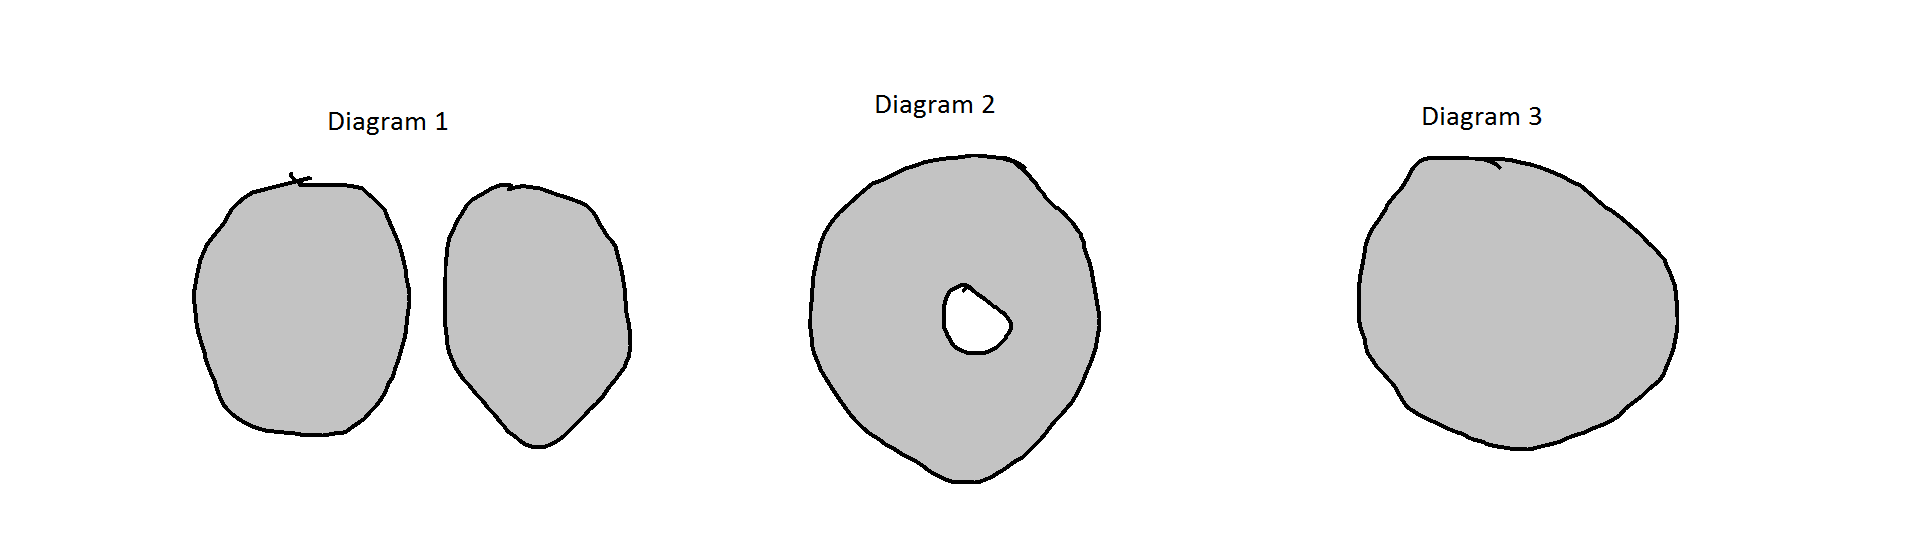
\includegraphics[scale=0.3]{CM_01}

Among the above three diagrams, the first is not connected, the second is not simply-connected, and the third is simply-connected.

\begin{defi}
The \emph{extended complex plane} $\C^*=\C \cup \{\infty\}$. We can reach the 'point at infinity' by going off in any direction in the plane, and all are equivalent.

Conceptually, we may use the \emph{Riemann sphere}, which is a sphere resting on the complex plane with its 'South Pole' $S$ at $z=0$.
\end{defi}

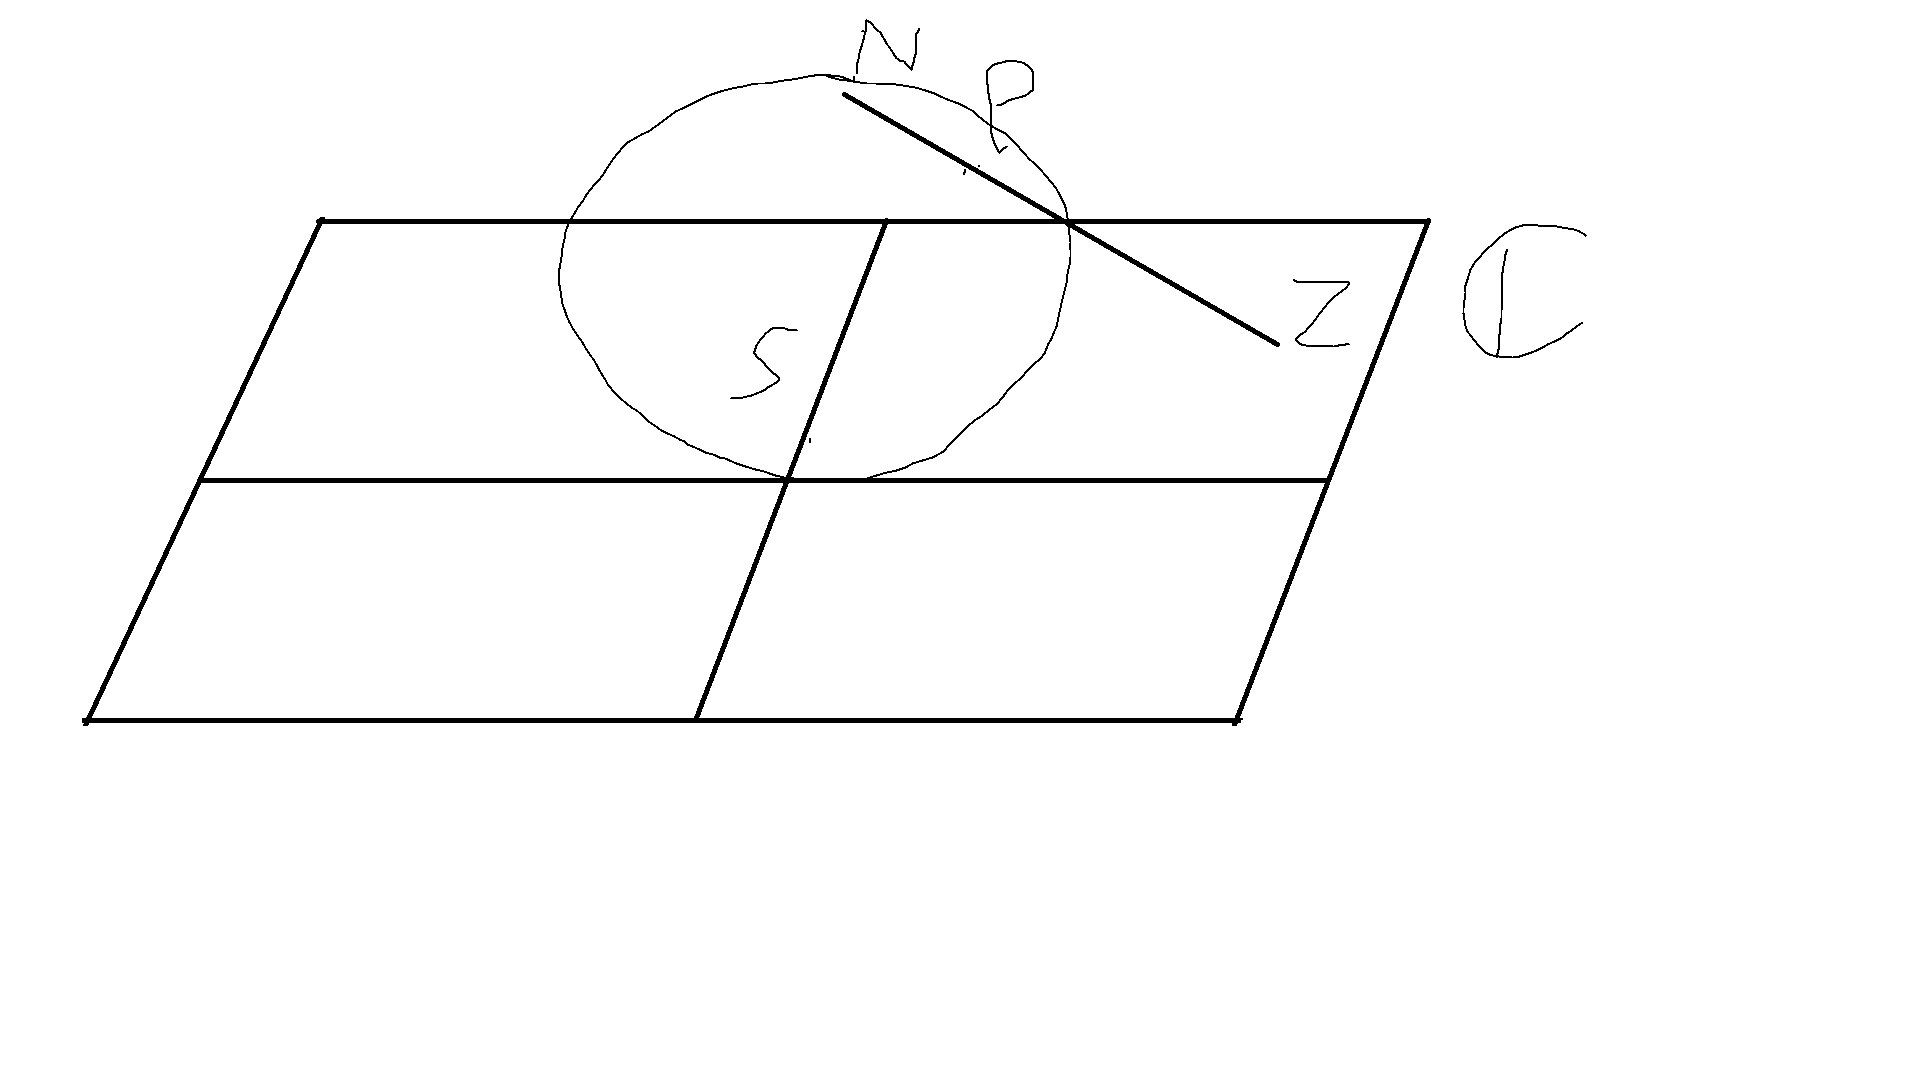
\includegraphics[scale=0.3]{CM_02}

For any point $z$ in $\C$, drawing a line through the 'North Pole' $N$ of the sphere to $z$, and noting where this intersects the sphere, specifies an equivalent point $P$ on the sphere. Then $\infty$ is equivalent to the 'North Pole' itself.

To investigate properties of $\infty$, we use the substitution $\zeta = \frac{1}{z}$. A function $f(z)$ is said to have a particular property at $\infty$ if $f(\frac{1}{\zeta})$ has that same property at $\zeta = 0$. 

\subsection{Complex Differentiation}
Recall the definition of differentiation for a real function $f(x)$:
\begin{equation*}
\begin{aligned}
f'(x) = \lim_{\delta x \to 0} \frac{f(x+\delta x)-f(x)}{\delta x}
\end{aligned}
\end{equation*}
It is implicitly that the limit must be the same whichever direction we approach from. Consider $|x|$ at $x=0$ for example; if we approach from the right ($\delta x \to 0^+$), then the limit is $+1$, whereas from the left ($\delta x \to 0^-$), it is $-1$. Because these limits are different, we say that $|x|$ is not differentiable at $x=0$.

Now extend the definition to complex functions $f(z):$ $f$ is differentiable at $z$ if
\begin{equation*}
\begin{aligned}
f'(z) = \lim_{\delta z\to 0} \frac{f(z+\delta z)-f(z)}{\delta z}
\end{aligned}
\end{equation*}
exists (and is therefore independent of the direction of approach -- but now there is an infinity of possible directions).

We say that $f$ is \emph{analytic} at a point $z$ if there exists a neighbourhood of $z$ throughout which $f'$ exists. The terms \emph{regular} and \emph{holomorphic} are also used. A function which is analytic throughout $\C$ is called entire.

The property of analyticity is in fact a surprisingly strong one! For example, two consequences include:\\
$\bullet$ If a function is analytic then it is differentiable infinitely many times (c.f. the existence of real functions which can be differentiated $N$ times but no more, for any given $N$).\\
$\bullet$ A bounded entire function is a constant (c.f. $\tanh x$ for $x \in \R$).

\begin{defi}
A \emph{singularity} of $f$ is a point at which it is \emph{not} analytic, or not even defined.
\end{defi}

\begin{thm} (Cauchy-Riemann Equations)\\
Separate $f$ and $z$ into real and imaginary parts:
\begin{equation*}
\begin{aligned}
f(z)=u(x,y)+iv(x,y)
\end{aligned}
\end{equation*}
where $z=x+iy$ and $u,v$ are real functions. Suppose that $f$ is differentiable at $z$. We may take $\delta z$ in any direction; first take it to be real, $\delta z = \delta x$. Then
\begin{equation*}
\begin{aligned}
f'(z) &= \lim_{\delta x \to 0} \frac{f(z+\delta x) - f(z)}{\delta x}\\
&=\lim_{\delta x\to 0} \frac{u(x+\delta x,y)+iv(x+\delta x,y) - u(x,y) - iv(x,y)}{\delta x}\\
&= \frac{\partial u}{\partial x} + i \frac{\partial v}{\partial x}
\end{aligned}
\end{equation*}
Now take $\delta z$ to be pure imaginary, i.e. $\delta z = i\delta y$. Then
\begin{equation*}
\begin{aligned}
f'(z) &= \lim_{\delta y \to 0} \frac{f(z+i\delta y) - f(z)}{i\delta y}\\
&= \lim_{\delta y \to 0} \frac{u(x,y+\delta y) + iv(x,y+\delta y) - u(x,y) - iv(x,y)}{i\delta y}\\
&= -i \frac{\partial u}{\partial y} + \frac{\partial v}{\partial y}
\end{aligned}
\end{equation*}

The two values for $f'(z)$ must be the same since $f$ is differentiable. So compare real and imaginary parts we get
\begin{equation*}
\begin{aligned}
\frac{\partial u}{\partial x} = \frac{\partial v}{\partial y},\\
\frac{\partial v}{\partial x} = -\frac{\partial u}{\partial y}
\end{aligned}
\end{equation*}
The \emph{Cauchy-Riemann equations}. The converse (that a function satisfying the CR equations is differentiable) is true only if we impose additional requirements, for example that the partial derivatives $u_x,u_y,v_x,v_y$ are continuous functions of $x$ and $y$ (together), in the sense described in Analysis II.
\end{thm}

\begin{eg} (Analytic functions)\\
(i) $f(z)=z$ is entire. We check $u=x,v=y$, and the $C-R$ equations are satisfied ($1=1$ and $0=0$).\\
(ii) $f(z)=e^z = e^x(\cos y+i\sin y)$ is entire since
\begin{equation*}
\begin{aligned}
\frac{\partial u}{\partial x} = e^x \cos y =\frac{\partial v}{\partial y},\\
\frac{\partial u}{\partial y} = -e^x \sin y = -\frac{\partial v}{\partial x}
\end{aligned}
\end{equation*}
And obviously the derivatives are all continuous. The derivative is
\begin{equation*}
\begin{aligned}
f'(z)=\frac{\partial u}{\partial x} + i\frac{\partial v}{\partial x} = e^x \cos y + ie^x \sin y = e^z
\end{aligned}
\end{equation*}
as expected.\\
(iii) $f(z)=z^n$ ($n$ a positive integer) is entire.\\
Writing $z=r(\cos\theta + i\sin\theta)$ we obtain $u=r^n \cos n\theta$ and $v=r^n \sin n\theta$. We can check the CR equations using $r=\sqrt{x^2+y^2}$ and $\tan \theta = \frac{y}{x}$. The derivative is $nz^{n-1}$ as expected!\\
(iv) Any rational function, i.e. $f(z) = \frac{P(z)}{Q(z)}$ where $P,Q$ are polynomials is analytic except at points where $Q(z)=0$. For instance, $f(z)=\frac{z}{z^2+1}$ is analytic except at $\pm i$.\\
(v) Many standard real functions can be extended naturally to complex functions and obey the usual rules for their derivatives: for example:\\
$\bullet$
\begin{equation*}
\begin{aligned}
\sin z \equiv \frac{e^{iz}-e^{-iz}}{2i}
\end{aligned}
\end{equation*}
has derivative
\begin{equation*}
\begin{aligned}
\cos z \equiv \frac{e^{iz}+e^{-iz}}{2}
\end{aligned}
\end{equation*}
We can also write
\begin{equation*}
\begin{aligned}
\sin z = \sin(x+iy) &= \sin x \cos iy + \cos x \sin iy\\
&=\sin x \cosh y + i \cos x \sinh y
\end{aligned}
\end{equation*}
Similarly for $\cos z$, $\sinh z$, $\cosh z$, etc.

$\bullet$ $\log z = \log|z|+i\arg z$ has derivative $\frac{1}{z}$.

$\bullet$ The product, quotient and chain rules hold in exactly the same way as for real functions. 
\end{eg}

\begin{eg} (Non-analytic functions)\\
(i) $f(z) = \Re(z)$. We have $u=x,y=0$. But $1 \neq 0$, so $f$ is not analytic anywhere.\\
(ii) $f(z) = |z|$ has $u=\sqrt{x^2+y^2}$ and $v=0$, and is also nowhere analytic.\\
(iii) $f(z) = \bar{z} = x-iy$ (complex conjugate) has $u=x, v=-y$. We have $1 \neq -1$, so $f$ is also nowhere analytic.\\
(iv) $f(z) = |z|^2 = x^2+y^2$ has $u=x^z+y^2$, $v=0$ are satisfied only at the origin. So $f$ is only differentiable at $z=0$. So $f$ is also nowhere analytic.
\end{eg}

\subsubsection{(*)Analytic continuation}
If we are given the values of an analytic function in some restricted region -- which could be rather small, such as a short curve somewhere in the complex plane -- then there is a \emph{unique} extension of the function to the rest of $\C$ that is still analytic. This extension might have some singularities, and might be multi-valued.\\
This fact can be useful in extending the domain of definition of a function. We shall see an example in section 5.2.

\subsection{Harmonic functions}
Suppose $f(z) = u+iv$ is analytic. Then
\begin{equation*}
\begin{aligned}
\frac{\partial^2 u}{\partial x^2} = \frac{\partial}{\partial x}(\frac{\partial u}{\partial x}) = \frac{\partial}{\partial x}(\frac{\partial v}{\partial y}) = \frac{\partial}{\partial y}(\frac{\partial v}{\partial x}) = \frac{\partial}{\partial y}(-\frac{\partial u}{\partial y}) = -\frac{\partial^2 u}{\partial y^2}
\end{aligned}
\end{equation*}
So $u$ satisfies Laplace's equation in two dimensions,
\begin{equation*}
\begin{aligned}
\nabla^2 u = \frac{\partial^2 u}{\partial x^2} + \frac{\partial^2 u}{\partial y^2} = 0
\end{aligned}
\end{equation*}
Similarly, so does $v$.

A function satisfying Laplace's equation in an open set is said to be \emph{harmonic} there.

Functions $u$ and $v$ satisfying the CR equations are called \emph{harmonic conjugates}. If we know one then we can find the other, up to a constant. For example, consider $u(x,y) = x^2-y^2$, which is easily verified to be harmonic. Its harmonic conjugate $v$ satisfies
\begin{equation*}
\begin{aligned}
\frac{\partial v}{\partial y} = \frac{\partial u}{\partial x} = 2x \implies v = 2xy+g(x)
\end{aligned}
\end{equation*}
for some function $g(x)$. So
\begin{equation*}
\begin{aligned}
-2y = \frac{\partial u}{\partial y} = -\frac{\partial v}{\partial x} = -2y - g'(x) \implies g'(x) = 0
\end{aligned}
\end{equation*}
So $g(x)$ is some constant $\alpha$. The corresponding analytic function whose real part is $u$ is therefore
\begin{equation*}
\begin{aligned}
f(z) &= x^2-y^2+i(2xy+\alpha)\\
&=(x+iy)^2+i\alpha\\
&=z^2+i\alpha
\end{aligned}
\end{equation*}

If the domain is not simply connected then this method might give a solution that is multi-valued. For example, if $u=\frac{1}{2}\log(x^2+y^2)$, which is harmonic in the domain $0 < |z| < 1$, the corresponding $f(z)$ is $\log z$.

\subsection{Multi-valued functions}
For $z = re^{i\theta}$, we define $\log z = \log r + i \theta$. There are therefore infinitely many values of $\log z$, for $\theta$ may take an infinity of values. For example,
\begin{equation*}
\begin{aligned}
\log i = \frac{\pi i}{2}, \frac{5\pi i}{2}, -\frac{3\pi i}{2},...
\end{aligned}
\end{equation*}
Depending on which choice of $\theta$ we make.

\subsubsection{Branch points}
Consider the three curves shown in the diagram.

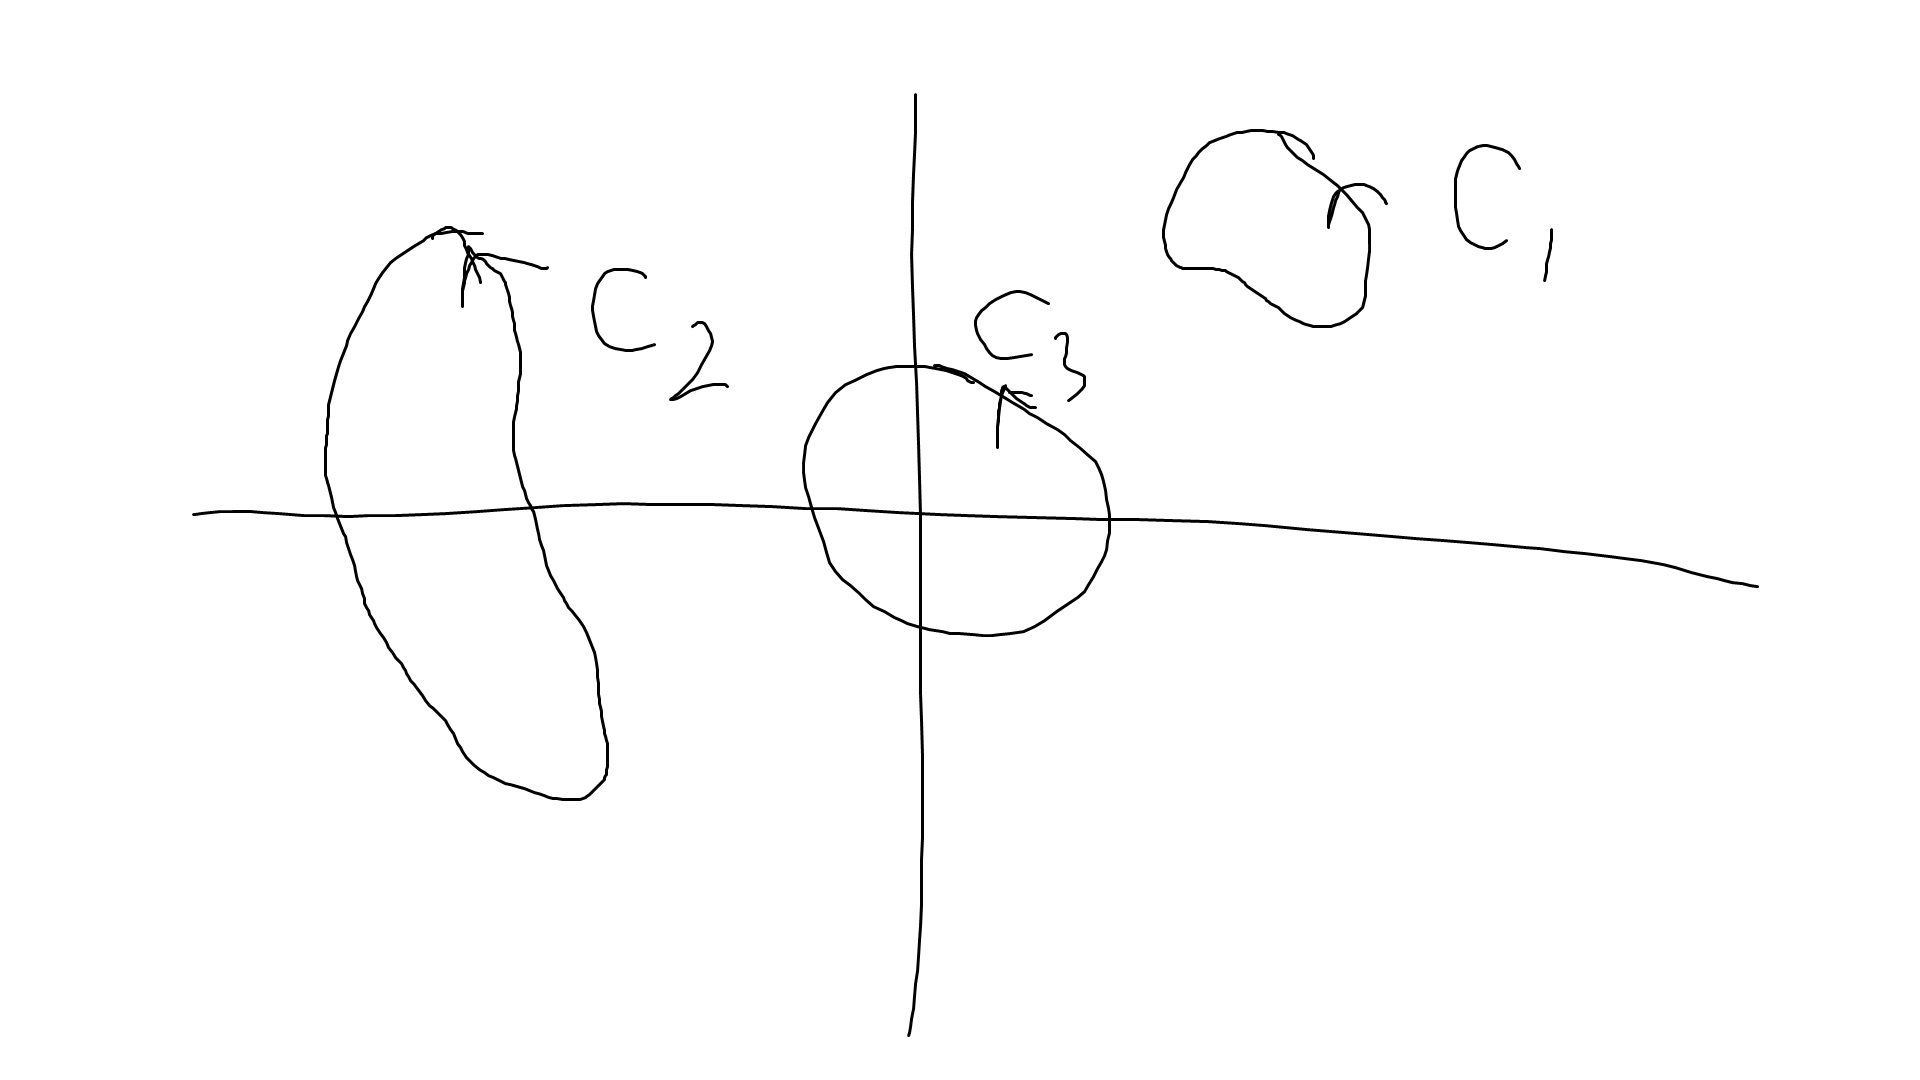
\includegraphics[scale=0.3]{CM_03}

On $C_1$, we could choose $\theta$ to be always in the range $(0,\frac{\pi}{2})$, and then $\log z$ would be continuous and single-valued (c.s.v.) going around $C_1$. On $C_2$, we could choose $\theta \in (\frac{\pi}{2},\frac{3\pi}{2})$ and $\log z$ would again be c.s.v. But for $C_3$, which encircles the origin, there is no such choice; whatever we do, $\log z$ cannot be made c.s.v. around $C_3$ (it must either 'jump' somewhere or be multi-valued).

A \emph{branch point} of a function -- here, the origin -- is a point which is impossible to encircle with a curve on which the function is both continuous and single-valued. The function is said to have a \emph{branch point singularity} at that point.

\begin{eg}
(i) $\log(z-a)$ has a branch point at $z=a$.\\
(ii) $\log (\frac{z-1}{z+1}) = \log(z-1) - \log(z+1)$ has two branch points at $\pm 1$.\\
(iii) $z^\alpha = r^\alpha e^{i\alpha \theta}$ has a branch point at the origin for $\alpha \not\in \Z$. Consider a circle of radius $r_0$ centred at $O$, and suppose WLOG that we start at $\theta = 0$ and go once round anti-clockwise.\\
$\theta$ must vary continuously to ensure continuity of $e^{i\alpha\theta}$, so as we get back almost to where we started, $\theta$ will approach $2\pi$. But then there will be a jump in $\theta$ back to $0$ (to satisfy the single-valued requirement) and hence a jump in $z^\alpha$ from $r_0^\alpha e^{2\pi i\alpha}$ to $r_0^\alpha$ (note that if $\alpha \in \Z$ then $e^{2\pi i\alpha} = 1$, so there's no jump). We cannot, therefore, make $z^\alpha$ c.s.v. on the circle.\\
(iv) $\log z$ also has a branch point at $\infty$, because if $\zeta = \frac{1}{z}$ (see section 1.1), $\log z = -\log \zeta$ which has a branch point at $\zeta = 0$. Similarly, $z^\alpha$ has a branch point at $\infty$ for $\alpha \not \in \Z$.\\
(v) $\log(\frac{z-1}{z+1})$ does not have a branch point at $\infty$, because if $\zeta = \frac{1}{z}$ then $\log(\frac{z-1}{z+1}) = \log(\frac{1-\zeta}{1+\zeta})$. For $\zeta$ close to zero, $\frac{1-\zeta}{1+\zeta}$ remains close to $1$ and therefore well away from the branch point of $\log$ at the origin. So we can encircle $\zeta = 0$ without $\log \frac{1-\zeta}{1+\zeta}$ being discontinuous.
\end{eg}

\subsubsection{Branch cuts}
If we wish to ensure that $\log z$ is c.s.v. on any curve, therefore, we must stop curves from encircling the origin. We do this by introducing a \emph{branch cut} from $-\infty$ on the real axis to the origin. No curve is allowed to cross this cut.

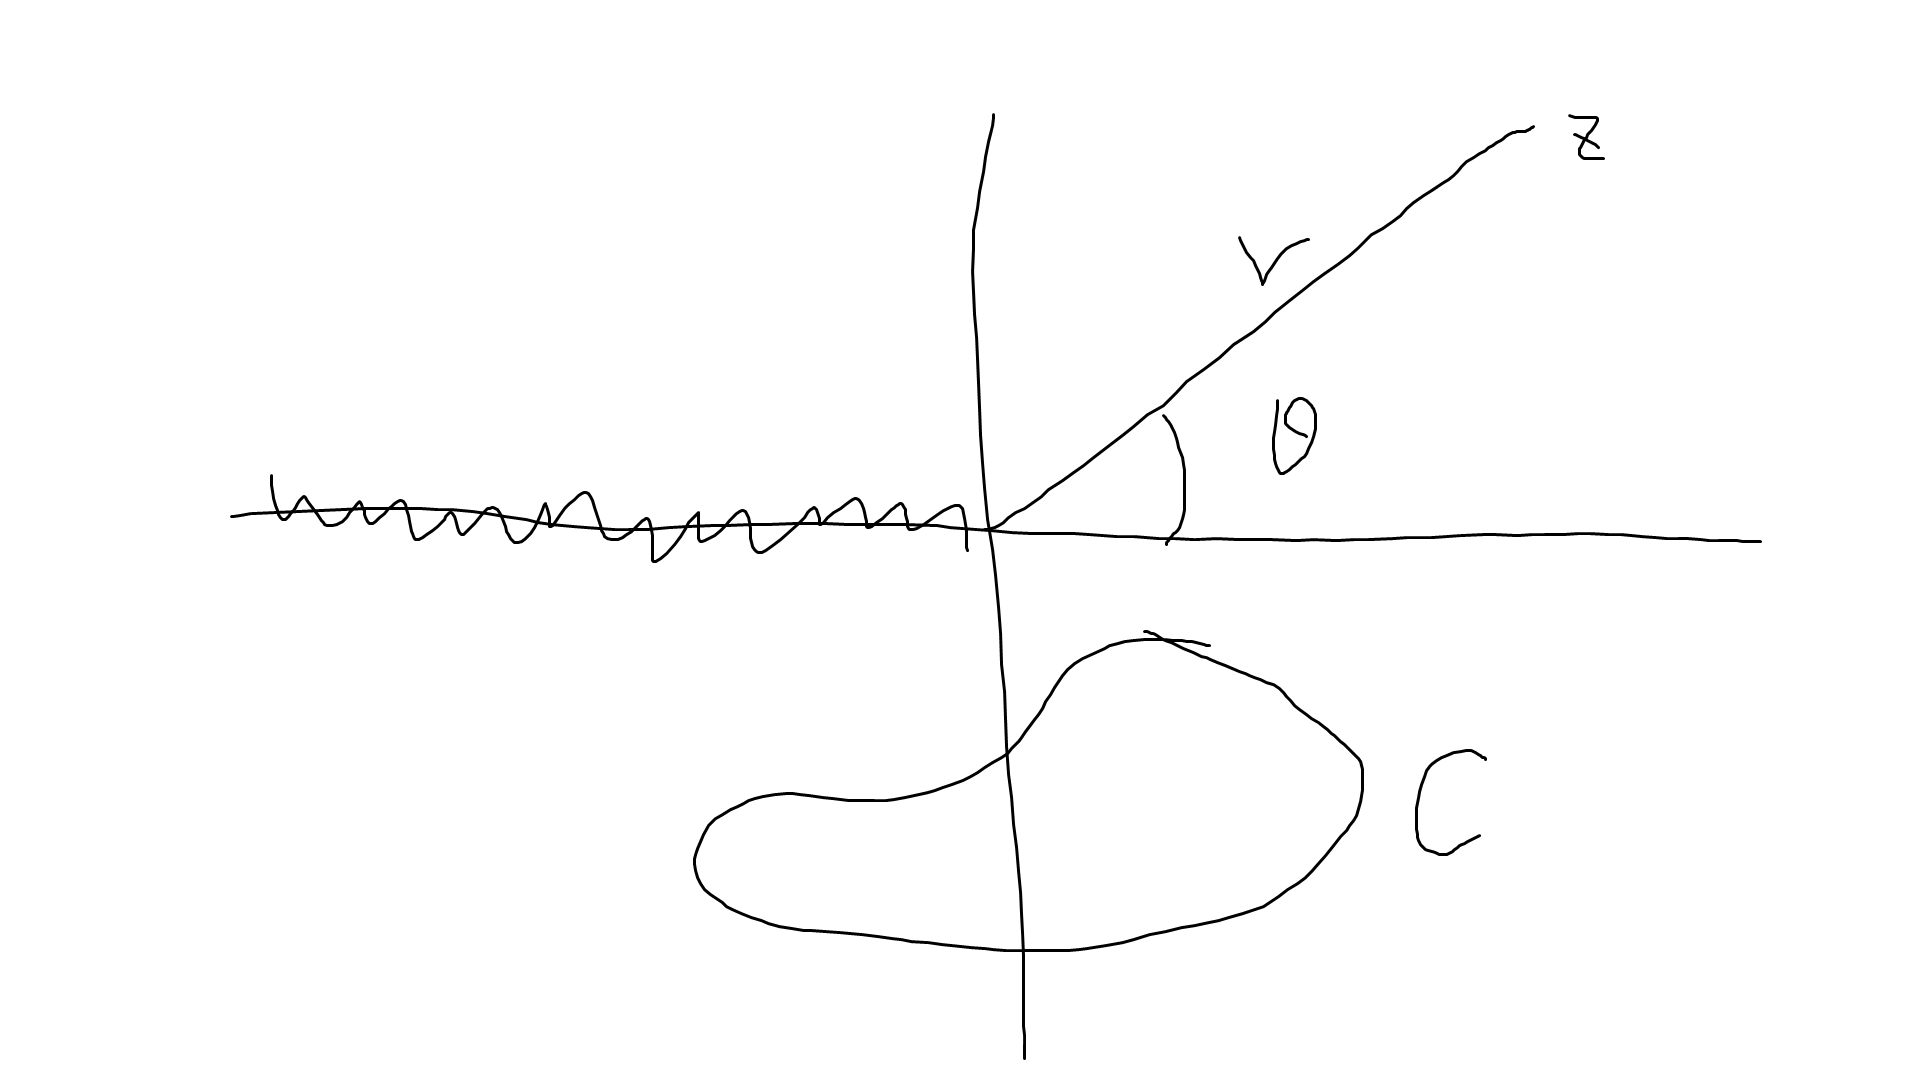
\includegraphics[scale=0.4]{CM_04}

We can then decide to fix on values of $\theta$ lying in the range $(-\pi,\pi]$ \emph{only}, and we have defined a \emph{branch} of $\log z$ which is c.s.v. on any curve $C$ that doesn't cross the cut. This branch is analytic everywhere with derivative $\frac{1}{z}$) \emph{except} on the negative real axis, where it is not even continuous, and at the branch point itself.

The cut described above is the canonical (i.e. standard) branch cut for $\log z$, and the branch of $\log z$ is called the \emph{principal value of the logarithm}.

What are the values of $\log z$ just above and below the branch cut? Consider a point on the negative real axis, $z=x$, $x<0$. Just above the cut, at $z=x+i0^+$, $\theta = \pi$ (in the limit) so
\begin{equation*}
\begin{aligned}
\log z = \log|x| + i\pi
\end{aligned}
\end{equation*}
Just below it, at $z=x+i0^-$, $\log z = \log |x| - i\pi$.

This is not the only possible branch of $\log z$, for example:

(a) We could place the branch cut along the negative imaginary axis and choose $\theta \in (-\frac{\pi}{2},\frac{3\pi}{2}]$.\\
(b) With a branch cut along the negative real axis, we could choose $\theta \in (\pi,3\pi]$. Then $\log 1 = 2\pi i$.\\
(c) With the branch as illustrated, it is more difficult to write down the exact choice of $\theta$. But this is equally valid.

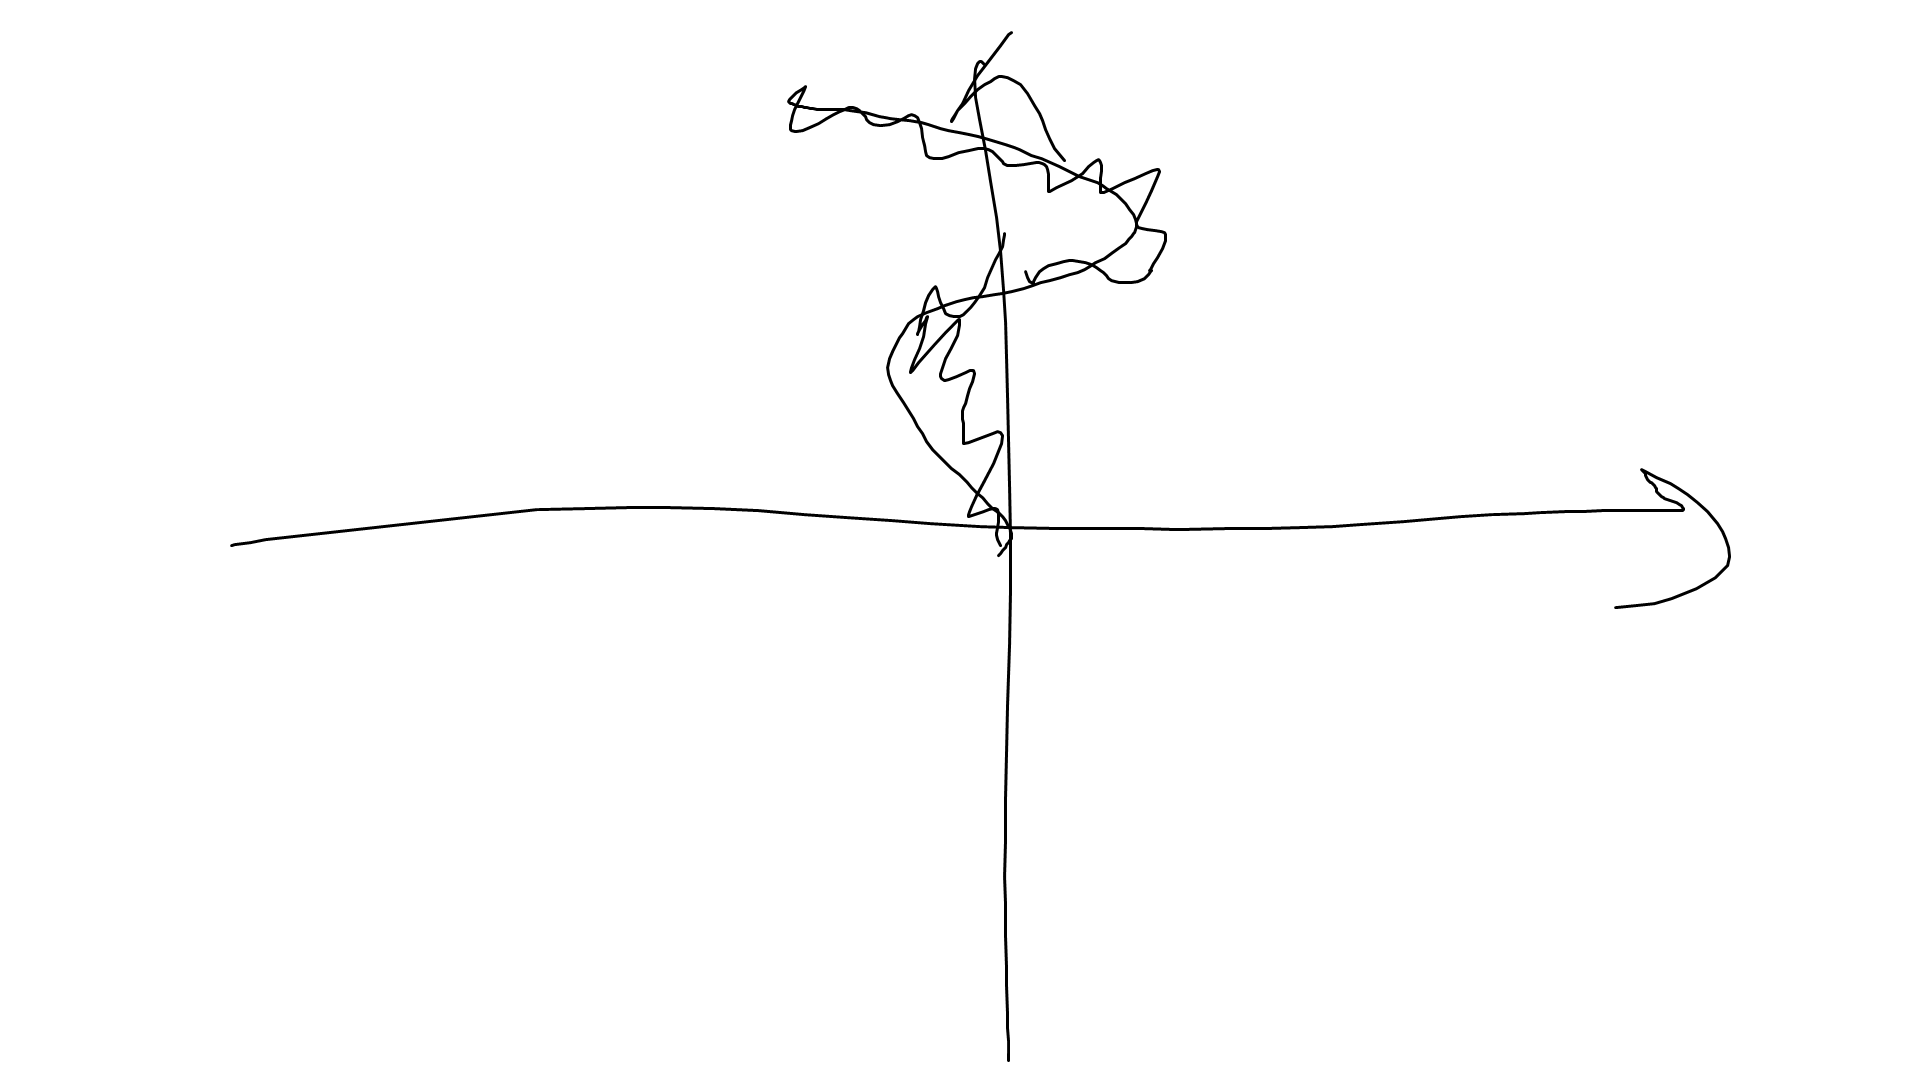
\includegraphics[scale=0.3]{CM_05}

Any branch cut that stops curves wrapping round the branch point will do.

Exactly the same considerations (and possible branch cuts) apply for $z^\alpha = r^\alpha e^{i\alpha\theta}$, $\alpha \not\in \Z$. Another way of seeing this is to note that $z^\alpha = e^{\alpha \log z}$.

Whenever a problem requires the use of a branch, it is important to specify it clearly. This can be done in two ways:\\
$\bullet$ Define the function and parameter range explicitly, e.g.
\begin{equation*}
\begin{aligned}
\Log z = \log|z| + i\arg z, \arg z \in (-\pi,\pi]
\end{aligned}
\end{equation*}
$\bullet$ Specify the location of the branch cut and give the value of the required branch at a single point not on the cut. The values everywhere else are then defined uniquely by continuity. For example, $\log z$ with a branch cut along $\R^-$ and $\log 1 \equiv 0$.

Note that a branch cut \emph{alone} does not specify a branch (compare (b) above with the principal branch, which is a different branch even though it uses the same branch cut), nor a single value of the function sufficient by itself (compare (a) and (c) above).

\subsubsection{Riemann Surfaces*}
Riemann imagined different branches as separable copies of $\C$, all stacked on top of each other but each one joined to the next at the branch cut. This structure is a Riemann surface.

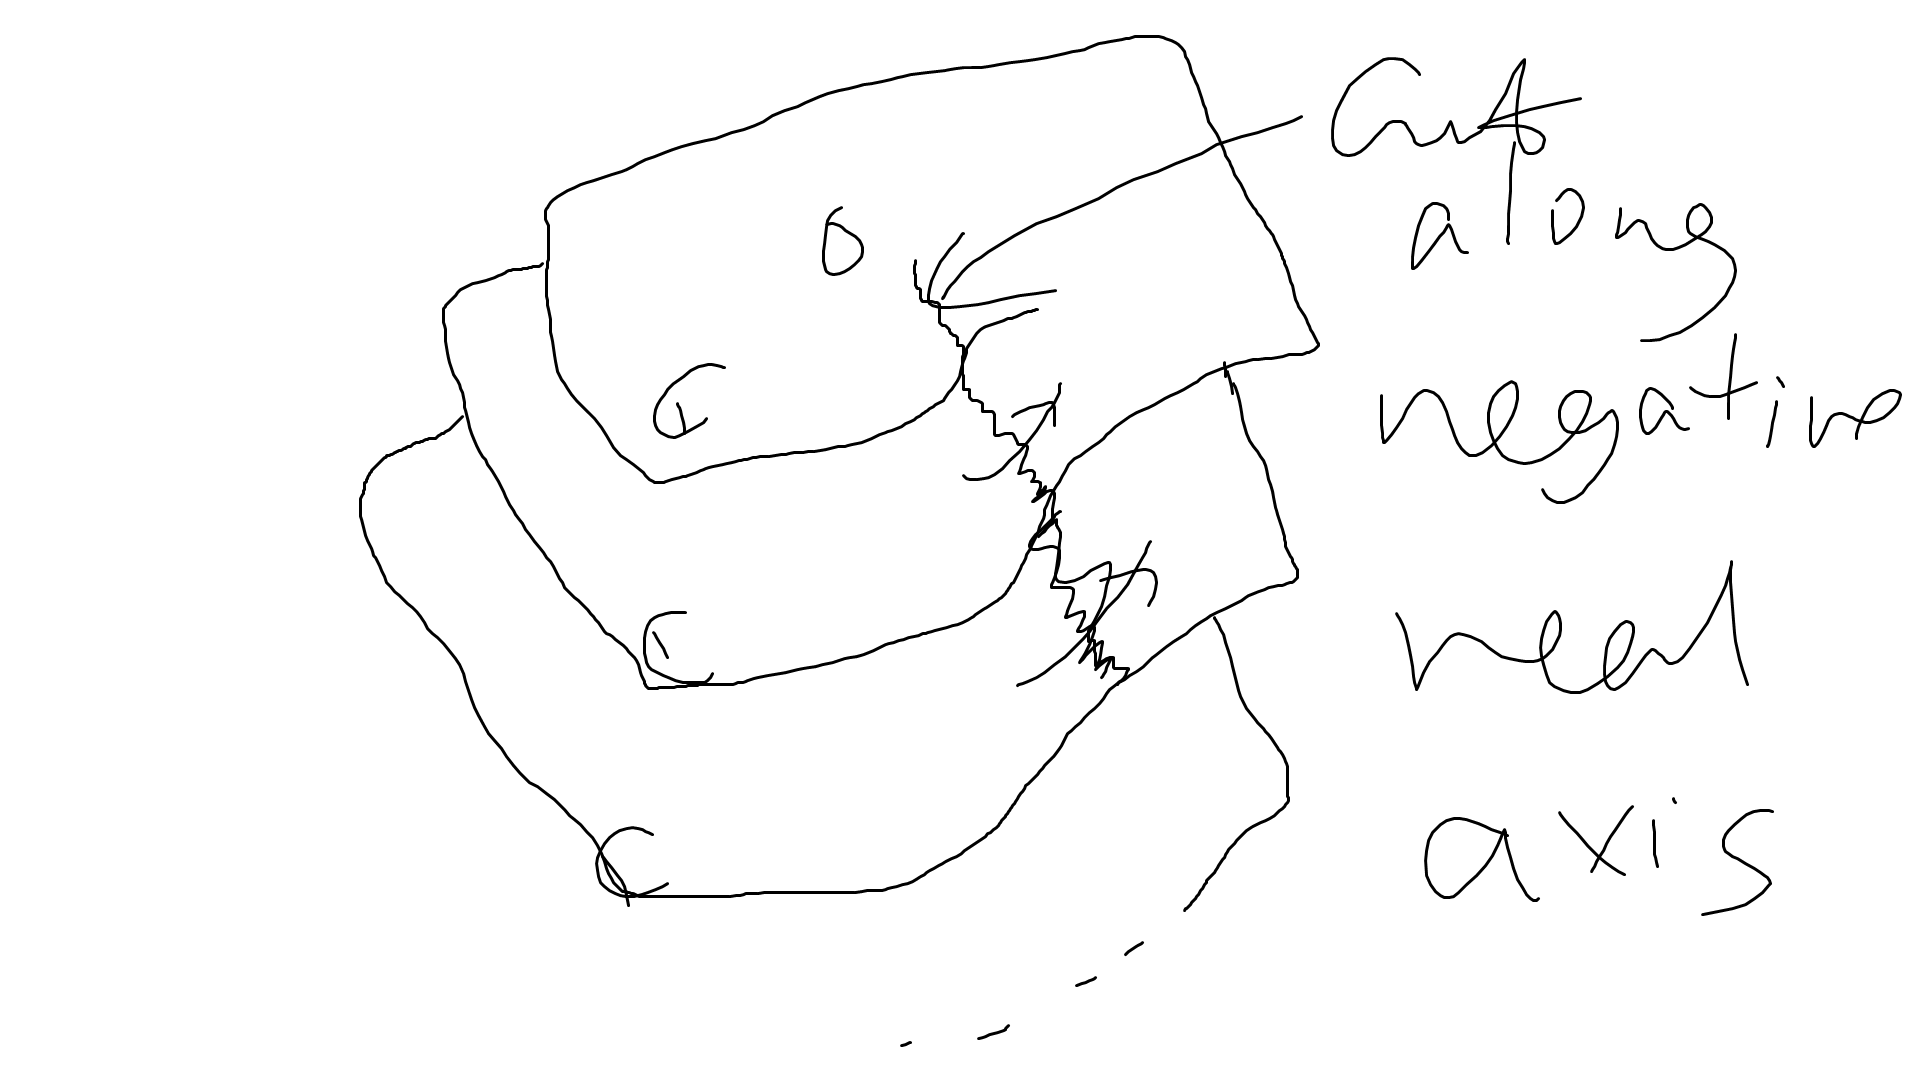
\includegraphics[scale=0.3]{CM_06}

\subsubsection{Multiple Branch Cuts}
When there is more than one branch point, we may need more than one branch cut. For
\begin{equation*}
\begin{aligned}
f(z) = \{z(z-1) \}^{1/3}
\end{aligned}
\end{equation*}
there are branch points at $0$ and $1$, so we need two branch cuts; a possibility is shown below. Then no curve can wrap around either $0$ or $1$.

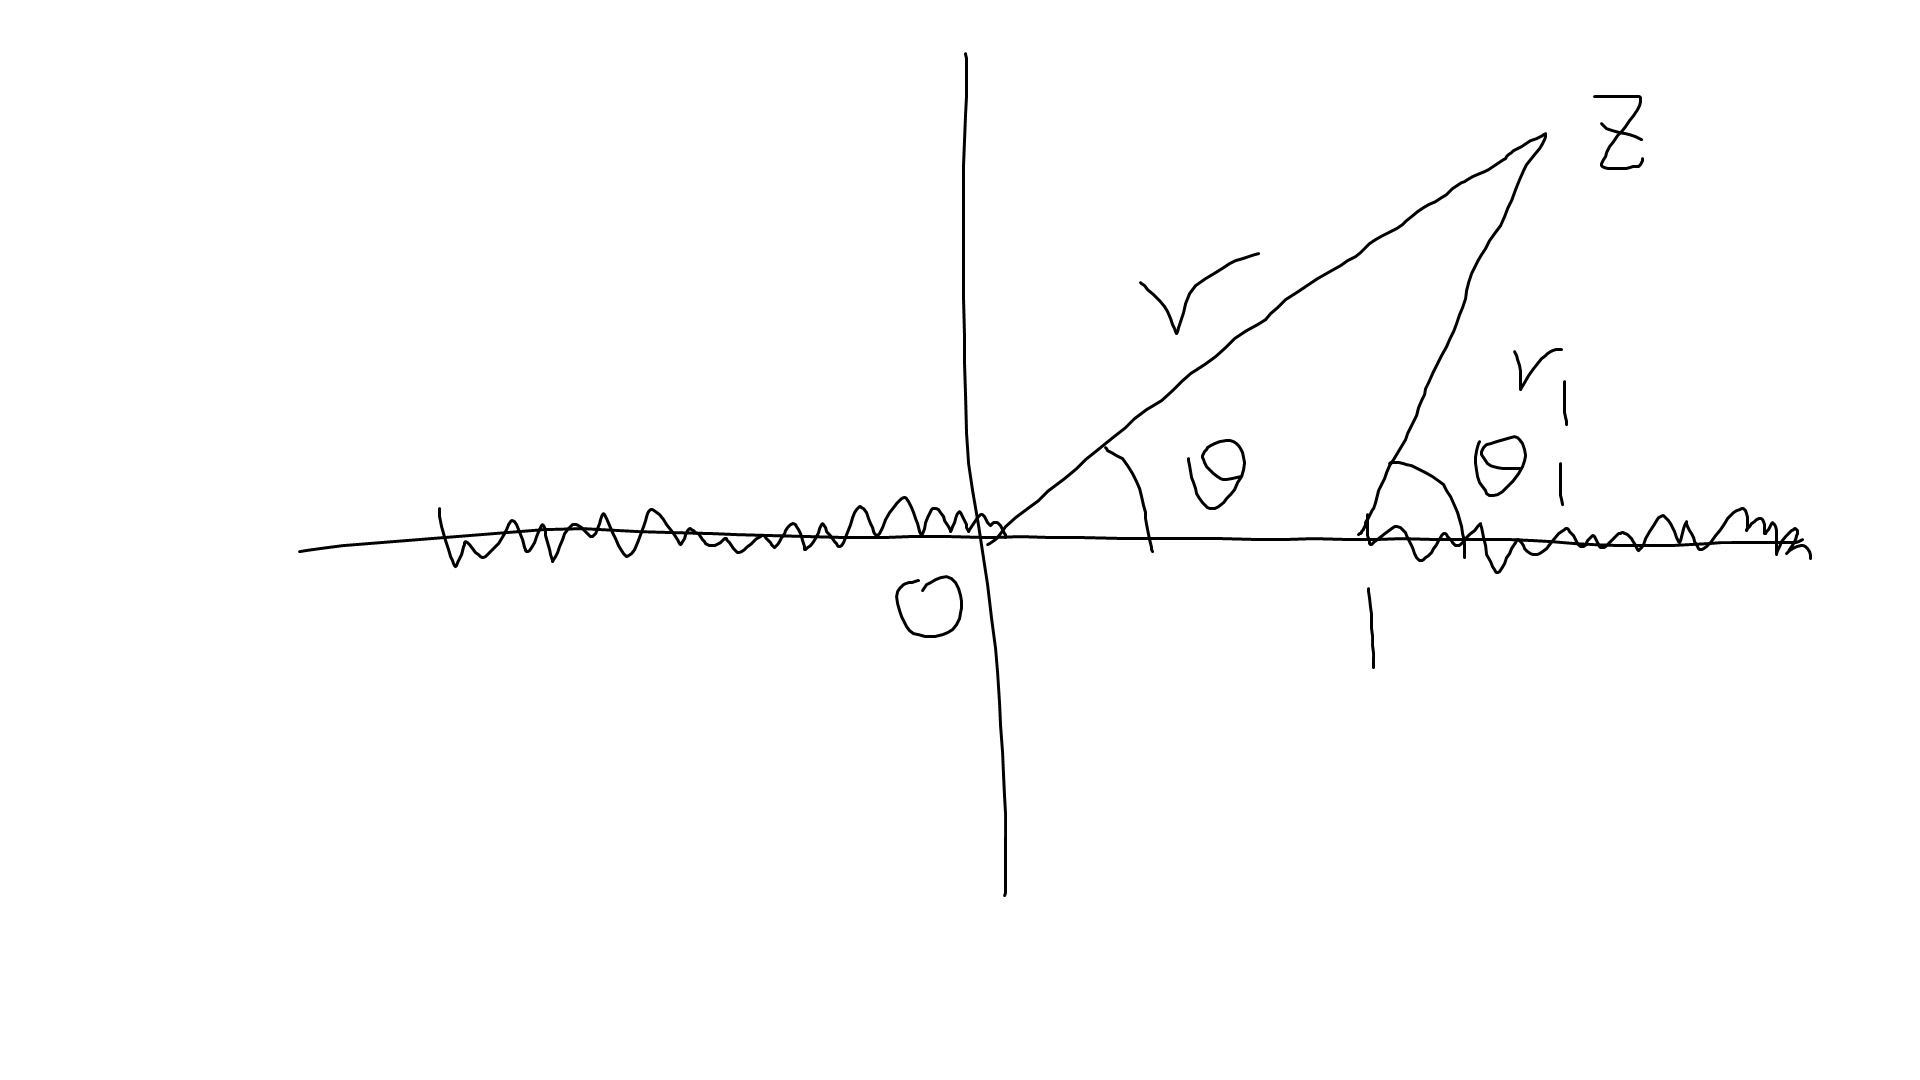
\includegraphics[scale=0.4]{CM_07}

For any $z$, write $z = re^{i \theta}$ and $z-1$ = $r_1 e^{i\theta}$, with $\theta \in (-\pi,\pi]$, $\theta_1 \in [0,2\pi)$, and define
\begin{equation*}
\begin{aligned}
\{ z(z-1\}^{1/3} = \sqrt[3]{rr_1} e^{i(\theta+\theta_1)/3}.
\end{aligned}
\end{equation*}
This is continuous so long as we don't cross either branch cut.

Sometimes we need fewer branch cuts than we might think: wee the worked example.

\subsection{M$\ddot{o}$bius maps}
The M$\ddot{o}$bius map
\begin{equation*}
\begin{aligned}
z \to w=\frac{az+b}{cz+d}, ad-bc \neq 0
\end{aligned}
\end{equation*}
is analytic except at $z=-\frac{d}{c}$. It can be useful to consider it as a map from $\C^*$ to $\C^*$ ($\C^* = \C \cup \{\infty\}$), with $-\frac{d}{c} \to \infty$ and $\infty \to \frac{a}{c}$. It is then bijective, the inverse being
\begin{equation*}
\begin{aligned}
w \to z=\frac{-dw+b}{cw-a}
\end{aligned}
\end{equation*}
which is another M$\ddot{o}$bius map.

A circline is either a circle or a line. M$\ddot{o}$bius maps take circlines to circlines.
\begin{proof}
Any circline can be expressed as a circle of Apollonius, $|z-z_1|=\lambda|z-z_2|$ where $z_1,z_2 \in \C$, $|lambda \in \R^+$ (recall Vectors and Matrices: the case $\lambda = 1$ corresponds to a line, $\lambda \neq 1$ to a circle). We then have
\begin{equation*}\tag{*}
\begin{aligned}
&\left|\frac{-dw+b}{cw-a} - z_1\right| = \lambda \left|\frac{-dw+b}{cw-a} - z_2\right|\\
\iff &|(cz_1+d)w-(az_1+b)| = \lambda |(cz_2+d)w-(az_2)+b|
\end{aligned}
\end{equation*}
If and only if
\begin{equation*}
\begin{aligned}
|w-w_1| = \lambda\left|\frac{cz_2+d}{cz_1+d}\right||w-w_2|
\end{aligned}
\end{equation*}
where $w_1 = \frac{az_1+b}{cz_1+d}$, $w_2 = \frac{az_2+b}{cz_2+d}$, which is another circle of Appolonius (This proof fails if either $cz_1+d$ or $cz_2+d$ vanishes; but in either of these cases, (*) trivially represents a circle).
\end{proof}

Geometrically it is clear that choosing three distinct points in $\C^*$ uniquely specifies a circline (If one of the points is $\infty$ then we have specified a straight line through the other two points).

Given $\alpha,\beta,\gamma,\alpha',\beta',\gamma' \in \C^*$, we can find a M$\ddot{o}$bius map which sends $\alpha \to \alpha'$, $\beta \to \beta'$, $\gamma \to \gamma'$.
\begin{proof}
The M$\ddot{o}$bius map
\begin{equation*}
\begin{aligned}
f_1(z) = \left(\frac{\beta - \gamma}{\beta - \alpha}\right) \frac{z-\alpha}{z-\gamma}
\end{aligned}
\end{equation*}
sends $\alpha \to 0$, $\beta \to 1$, $\gamma \to \infty$. Let
\begin{equation*}
\begin{aligned}
f_2(z) = \left(\frac{\beta' - \gamma'}{\beta' - \alpha'}\right) \frac{z-\alpha'}{z-\gamma'}
\end{aligned}
\end{equation*}
then $f^{-1}_2 \circ f_1$ is the required mapping. It is a M$\ddot{o}$bius map since M$\ddot{o}$bius maps form a group.

Putting all these results together, we conclude that we can find a M$\ddot{o}$bius map taking any given circline to any other.
\end{proof}

\subsection{Conformal map}
\begin{defi}
A \emph{conformal map} $f:U \to V$ where $U,V$ are \emph{open} subsets of $\C$, is one which is analytic with non-zero derivatives in $U$. Although not part of the definition, it is usual (and helpful) to require that $f$ be 1-1 from $U$ to $V$.

An alternative definition is that a conformal map is one that preserves the angle (in both magnitude and orientation) between intersecting curves. We shall show that our definition implies this. The converse is also true (proof omitted), so the two definitions are equivalent.
\begin{proof}
Suppose that $z_1(t)$ is a curve in $\C$ parameterised by $t \in \R$, which passes through a point $z_0$ when $t=t_1$. Suppose further that its tangent there, $z_1'(t)$, has a well-defined direction; then $z'_1(t_1) \neq 0$ and the curve makes an angle $\phi = \arg z'_1(t_1)$ to the $x$-axis at $z_0$.

Consider the image of the curve, $Z_1(t) = f(z_1(t))$. Its tangent direction at $t=t_1$ is
\begin{equation*}
\begin{aligned}
Z'_1(t_1) = z'_1(t_1) f'(z_1(t_1)) = z'_1(t_1) f'(z_0)
\end{aligned}
\end{equation*}
and therefore makes an angle with the $x$-axis of $\arg Z_1(t_1) = \arg(z'_1(t_1) f'(z_0)) = \phi+\arg f'(z_0)$ (noting that $\arg f'(z_0)$ exists since $f$ is conformal so $f'(z_0) \neq 0$). In other words, the tangent direction is rotated by $\arg f'(z_0)$.

Now if $z_2(t)$ is another curve passing through $z_0$, then its tangent direction will also be rotated by $\arg f'(z_0)$. The result follows.
\end{proof}
\end{defi}

Sometimes we don't know what $V$, the image of $f$ acting on $U$, is in advance. Often, the easiest way to find it is first to find the image of the boundary $\partial U$, which will form the boundary $\partial V$ of $V$; but, since this does not reveal upon which side of $\partial V$ $V$ lies, to then find the image of a single point of our choice within $U$, which will lie within $V$.

\begin{eg}
(i) The map $z \to az + b$, $a,b \in \C$, $a \neq 0$. It rotates by $\arg a$, enlarges by $|a|$, and translates by $b$, and is conformal everywhere.\\
(ii) $f(z) = z^2$ is a conformal map from
\begin{equation*}
\begin{aligned}
U = \{z:0<|z|<1,0<\arg z < \frac{\pi}{2}\}
\end{aligned}
\end{equation*}
to
\begin{equation*}
\begin{aligned}
V = \{w: 0 < |w| < 1, 0 < \arg w < \pi\}.
\end{aligned}
\end{equation*}

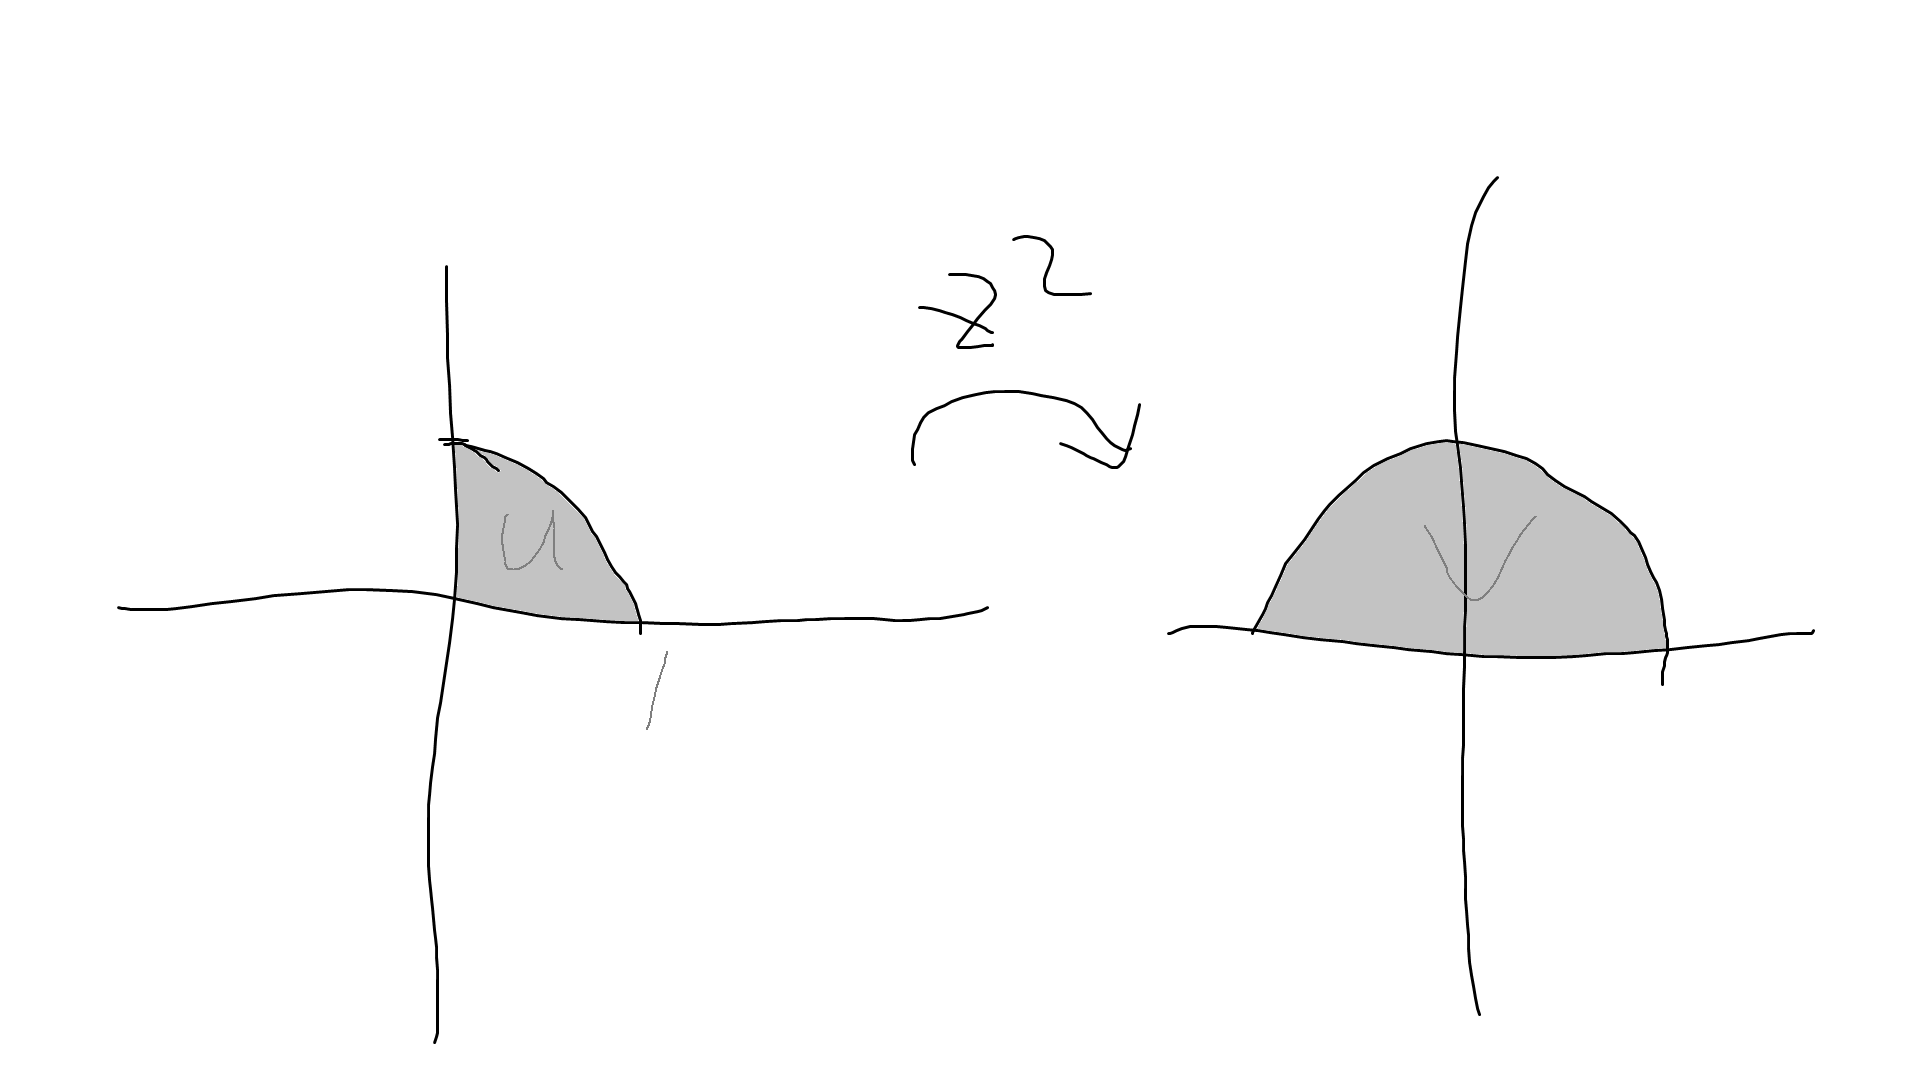
\includegraphics[scale=0.4]{CM_08}

Note that the right angle between the two boundary curves at $z=1$ is preserved because $f$ is conformal; similarly at $z=i$. But the right angle at $z=0$ is not preserved because $f'$ is not conformal there ($f'(0) = 0$). Fortunately this doesn't matter since $U$ is an \emph{open} set so does not include $0$.

(iii) Consider $U=\{z:\Re z<0\}$ and $V=\left\{w:-\frac{\pi}{4} < \arg w < \frac{\pi}{4} \right\}$.

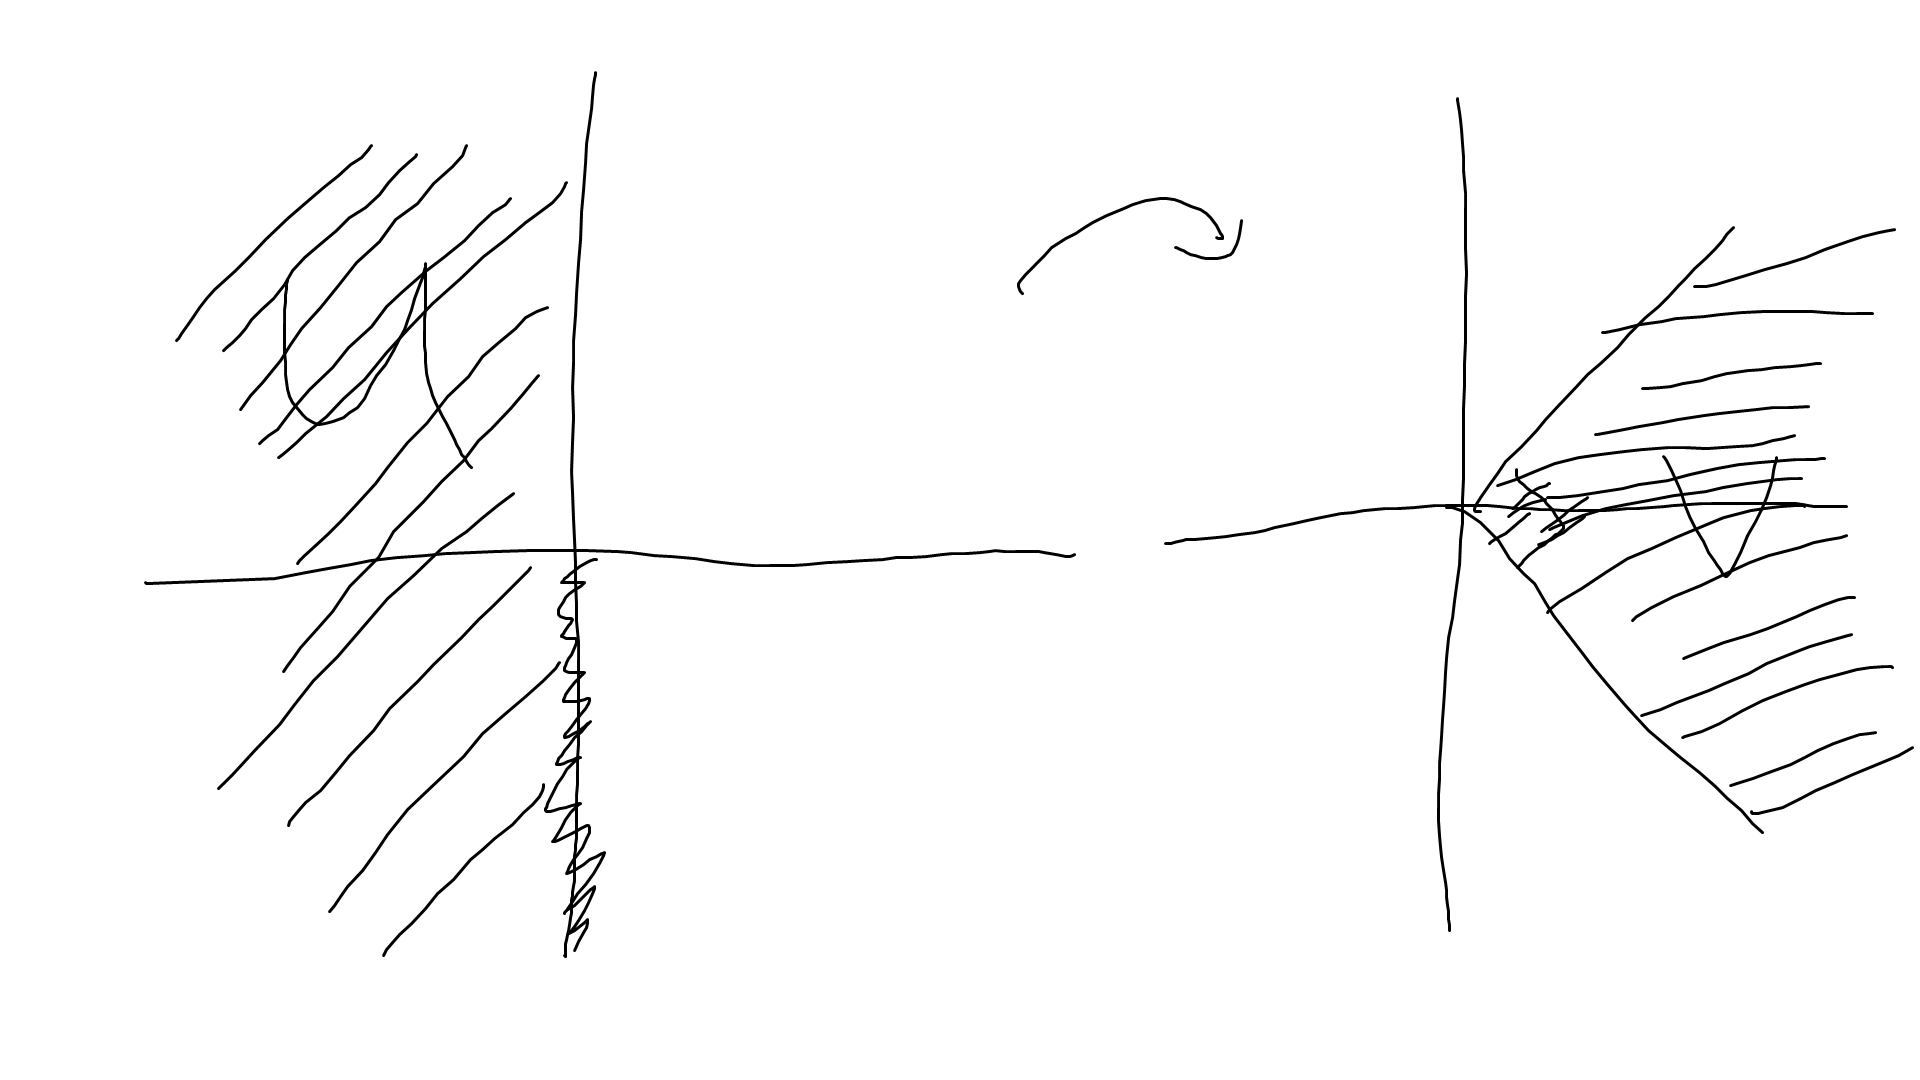
\includegraphics[scale=0.4]{CM_09}

We need to halve the angle, so try using $z^{1/2}$, for which we need to choose a branch. The branch cut must \emph{not} lie in $U$ (since $z^{1/2}$ is not analytic on the branch cut), so choose a cut along the negative imaginary axis: $re^{i\theta} \to \sqrt{r} e^{i\theta/2}$ where $\theta$ is chosen to lie in the range $(-\frac{\pi}{2},\frac{3\pi}{2}]$. Having defined this branch, we now apply $z^{1/2}$ to $U$ to produce the wedge $\{z':\frac{\pi}{4} < \arg z' < \frac{3\pi}{4}\}$; so we just need to rotate through $-\frac{\pi}{2}$. The final map is $f(z) = -iz^{1/2}$.

(iv) $e^z$ takes rectangles conformally to sectors of annuli:

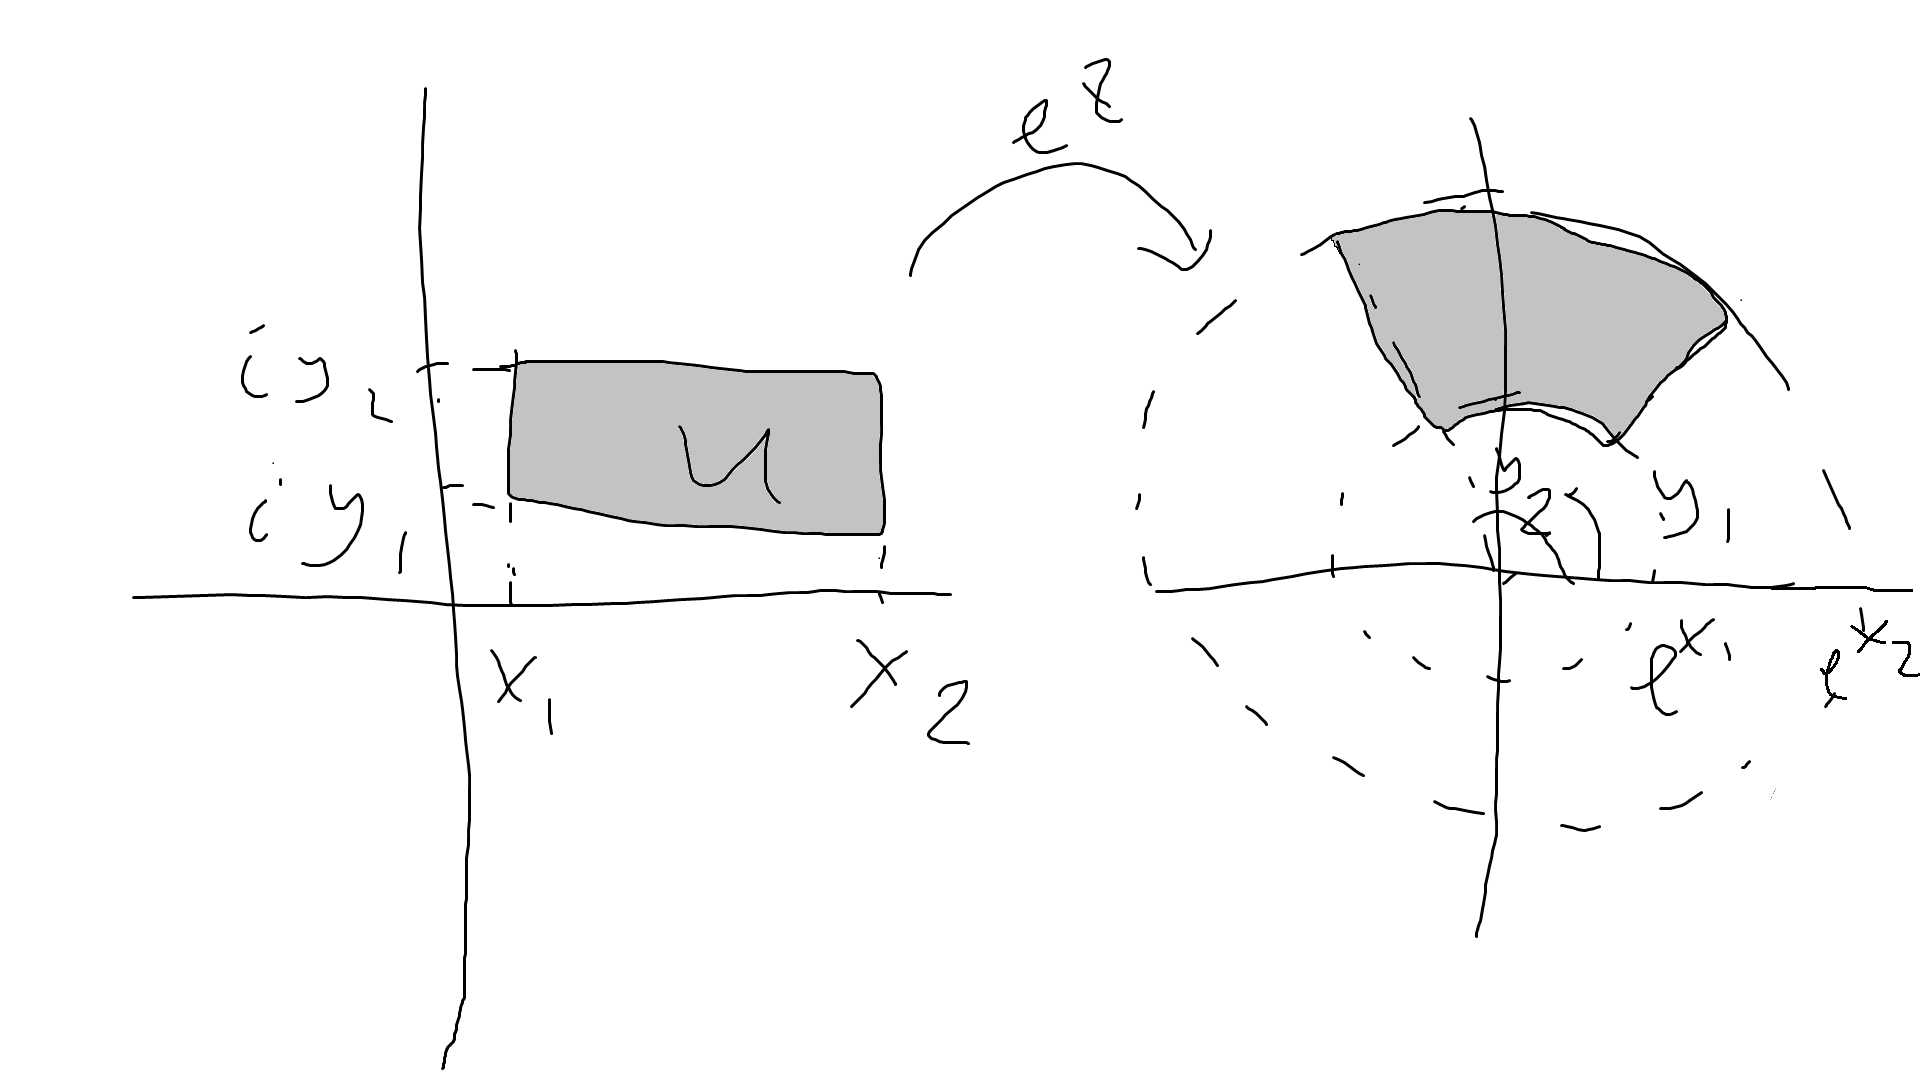
\includegraphics[scale=0.4]{CM_10}

With an appropriate choice of branch, $\log z$ does the reverse.

(v) M$\ddot{o}$bius maps (which are conformal everywhere except at the point that is sent to $\infty$) are very useful in taking circles, or parts of them, to straight lines, or vice versa.

Consider $f(z) = \frac{z-1}{z+1}$ acting on the unit disc $U=\{z:|z|<1\}$. The boundary of $U$ is a circle; the three points $-1,i$ and $i+1$ lie on this circle and are mapped to $\infty$, $i$ and $0$ respectively. Therefore (see section 1.5) the image of $\partial V$ is the imaginary axis; since $f(0) = -1$, we see that the image of $U$ is the left-hand half-plane.

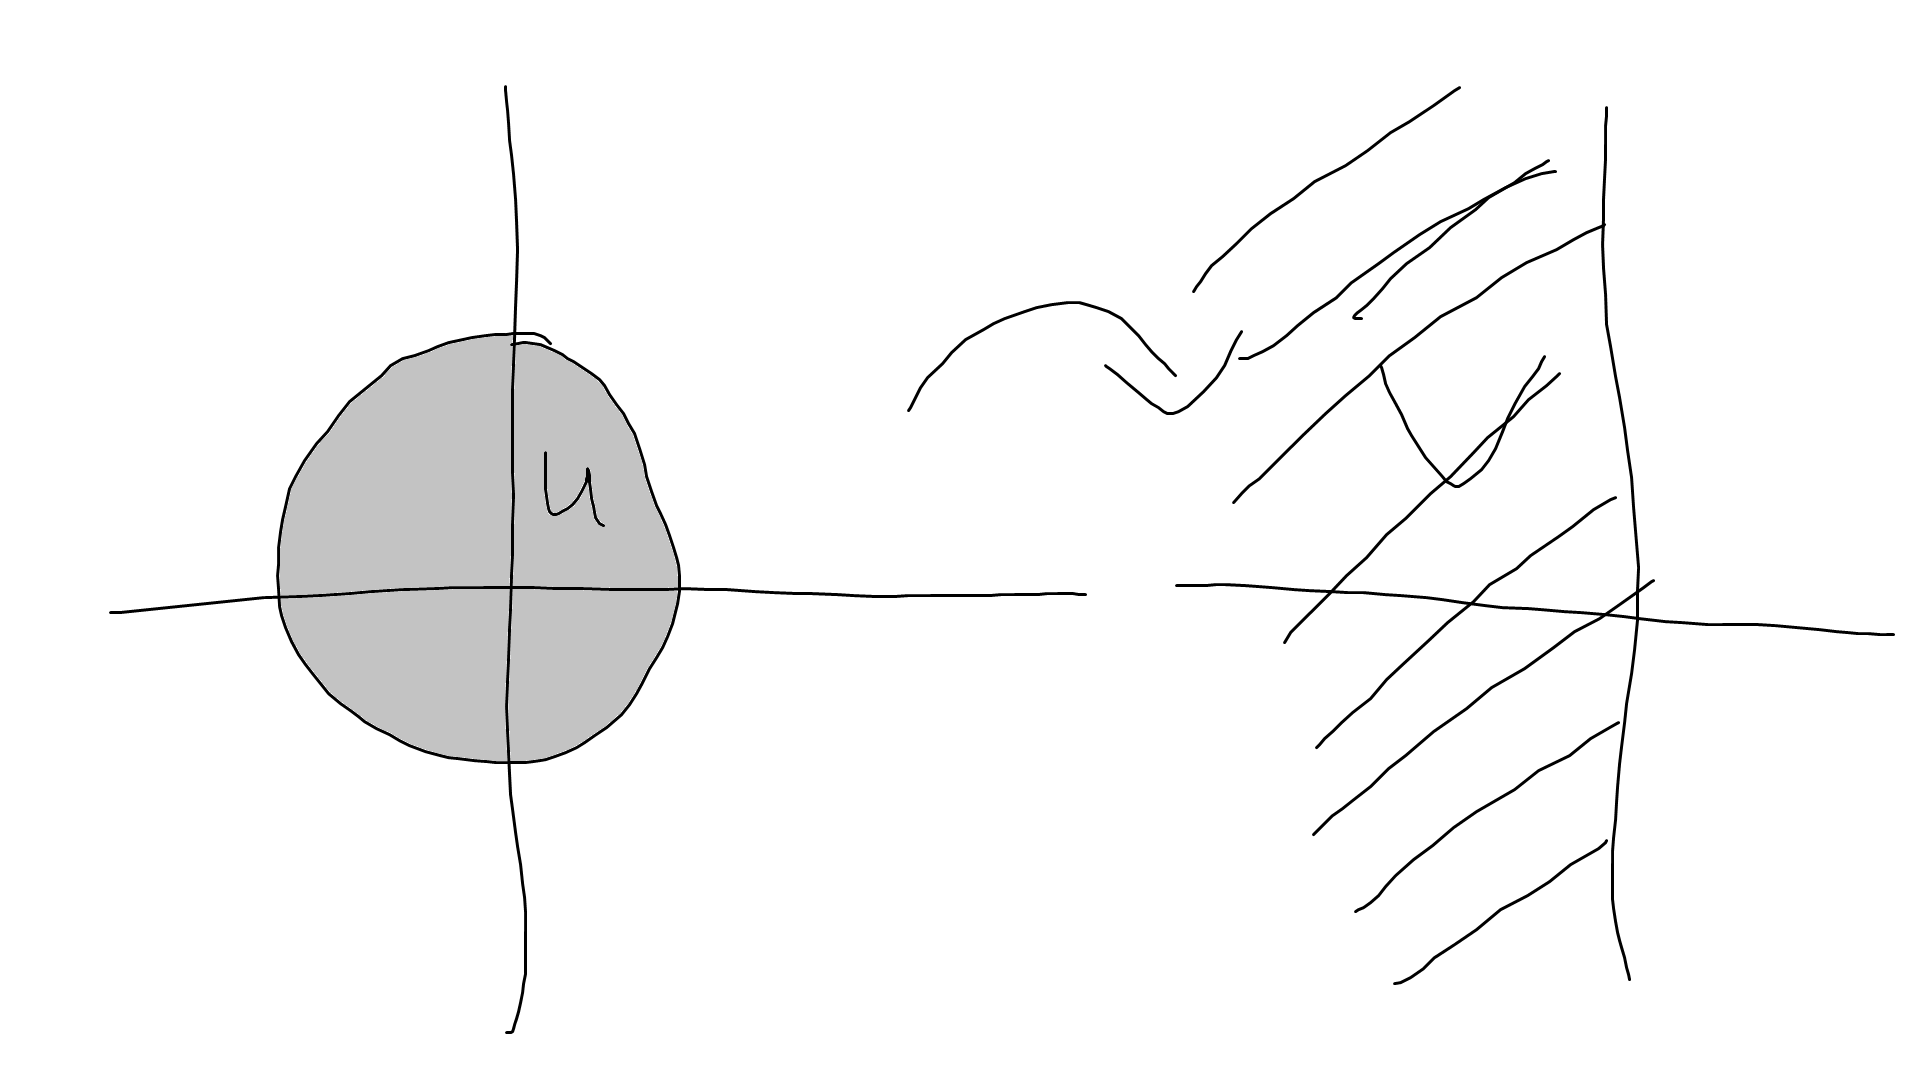
\includegraphics[scale=0.4]{CM_11}

*Alternative derivation: $w = \frac{z-1}{z+1} \iff z=-\frac{w+1}{w-1}$. So $|z| < 1 \iff |w+1|<|w-1|$, i.e. $w$ is closer to $-1$ than it is to $+1$.

In fact, this particular map can be deployed more generally on quadrants because it permutes $8$ divisions of the complex plane as follows:

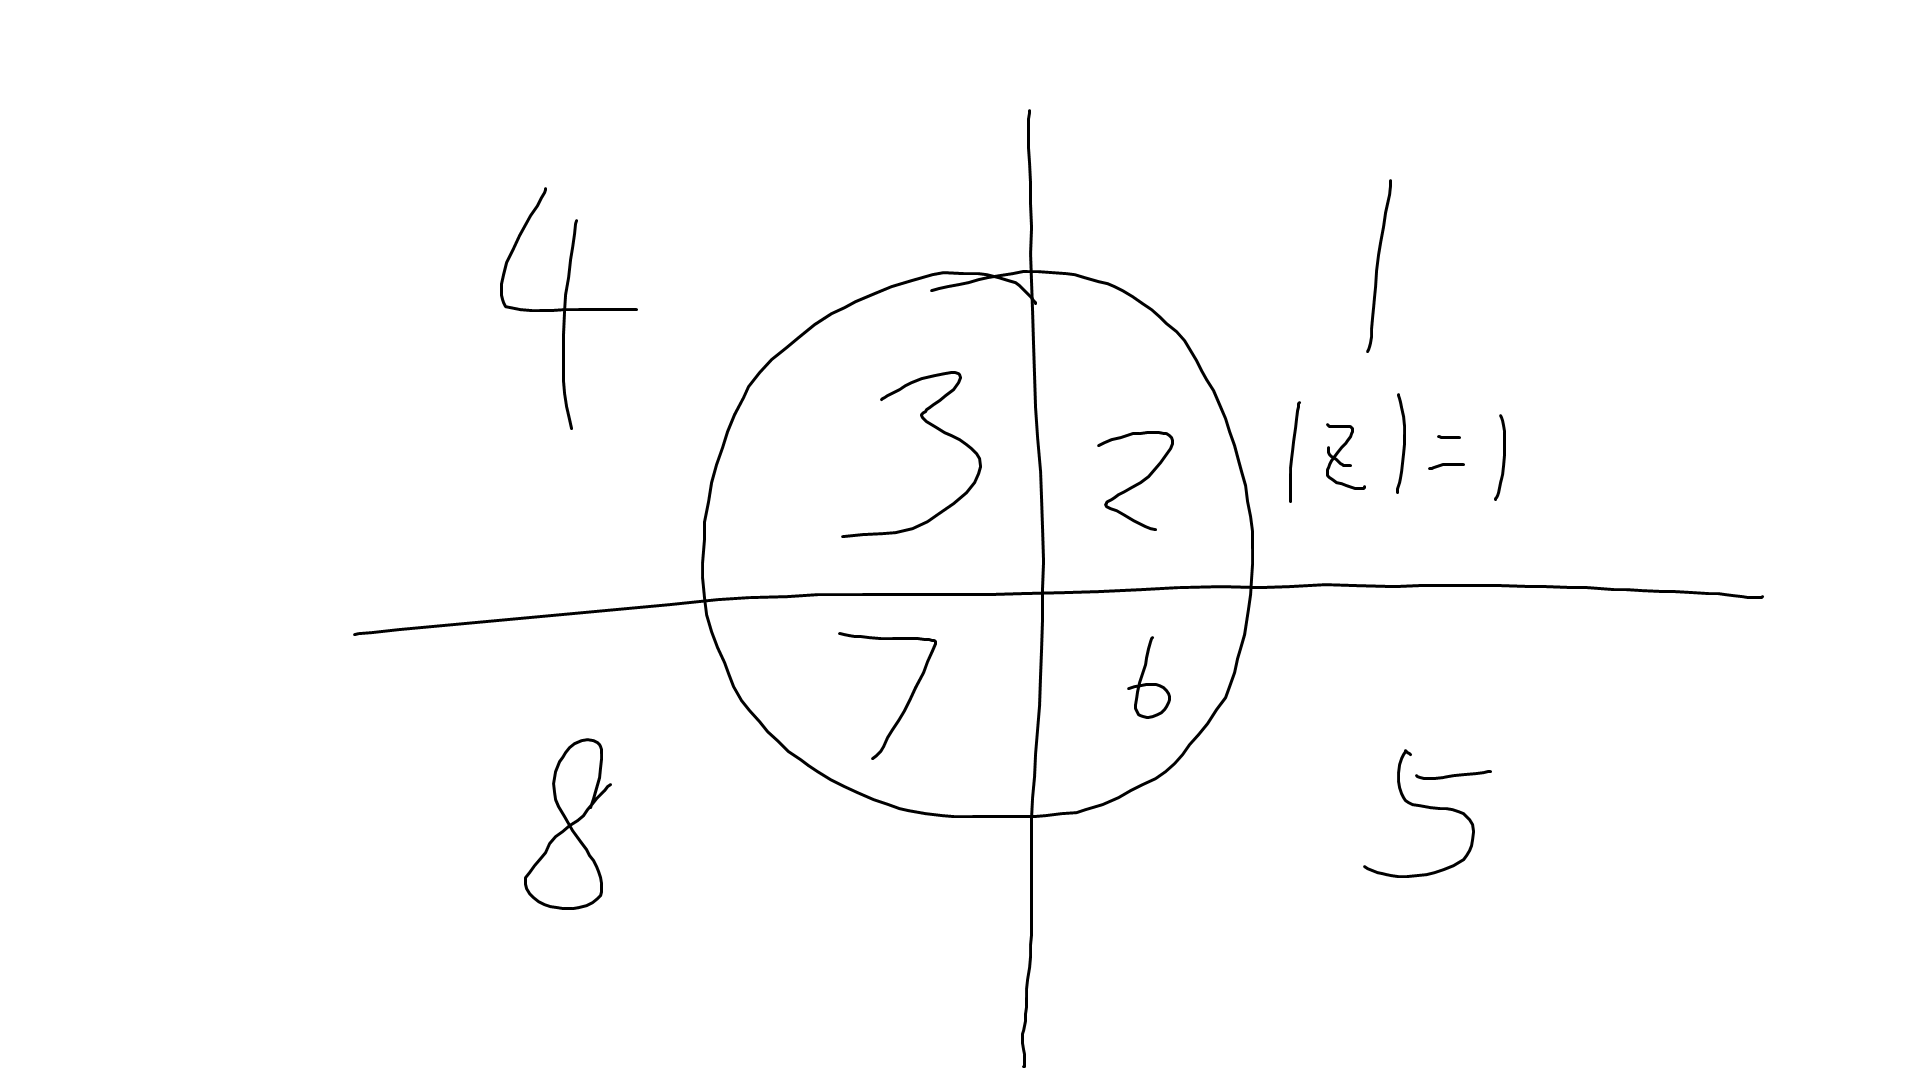
\includegraphics[scale=0.4]{CM_12}

$1 \to 2 \to 3 \to 4 \to 1$, $5 \to 6 \to 7 \to 8 \to 5$.

(vi) $f(z) = \frac{1}{z}$ is another M$\ddot{o}$bius map for acting on vertical or horizontal lines.
\end{eg}

In practice, complicated conformal maps are usually built up from individual building blocks, each a simple conformal map; the required map is the composition of these (note that the composition of conformal maps is still conformal, see the worked example).

\subsection{Solving Laplace's Equation using conformal maps}
The following algorithm can be used to solve Laplace's equation
\begin{equation*}
\begin{aligned}
\nabla^2 \phi(x,y) = 0
\end{aligned}
\end{equation*}
on a tricky domain $U \subset \R$ with given Dirichlet boundary conditions on $\partial U$. We identify subsets of $\R^2$ with subsets of $\C$ in the obvious manner.

1. Find a conformal map $f:U \to V$ where $U$ is now considered a subset of $\C$ and $V$ is a 'nice' domain of our choice. Our aim is to find a harmonic function $\Phi$ in $V$ that satisfies the same boundary conditions as $\phi$.\\
2. Map the boundary conditions on $\partial U$ directly to the equivalent points on $\partial V$.\\
3. Now solve $\nabla^2 \Phi =0$ in $V$ with the new boundary conditions.\\
4. The required harmonic function $\phi$ in $U$ is then given by
\begin{equation*}
\begin{aligned}
\phi(x,y) = \Phi(\Re f(x+iy), \Im f(x+iy)).
\end{aligned}
\end{equation*}
This works because, since $\Phi$ is harmonic, it is the real part of some complex analytic function $F(z) = \Phi(x,y) + i\Psi(x,y)$ where $z=x+iy$ (see section 1.3). Now $F(f(z))$ is analytic as it is a composition of analytic functions; so its real part, which is $\Phi(\Re f, \Im f)$, is harmonic.

\begin{eg}
Solve $\nabla^2 \phi = 0$ in the first quadrant of $\R^2$ subject to boundary condition $\phi(x,0) = 0$, $\phi(0,y) = 1$, where $x,y>0$, and with $\phi$ bounded near the origin and at $\infty$.\\
We choose $f(z) =\log(z)$ (principal branch) which maps $U$ to the strip $0<\Im z < \frac{\pi}{2}$.

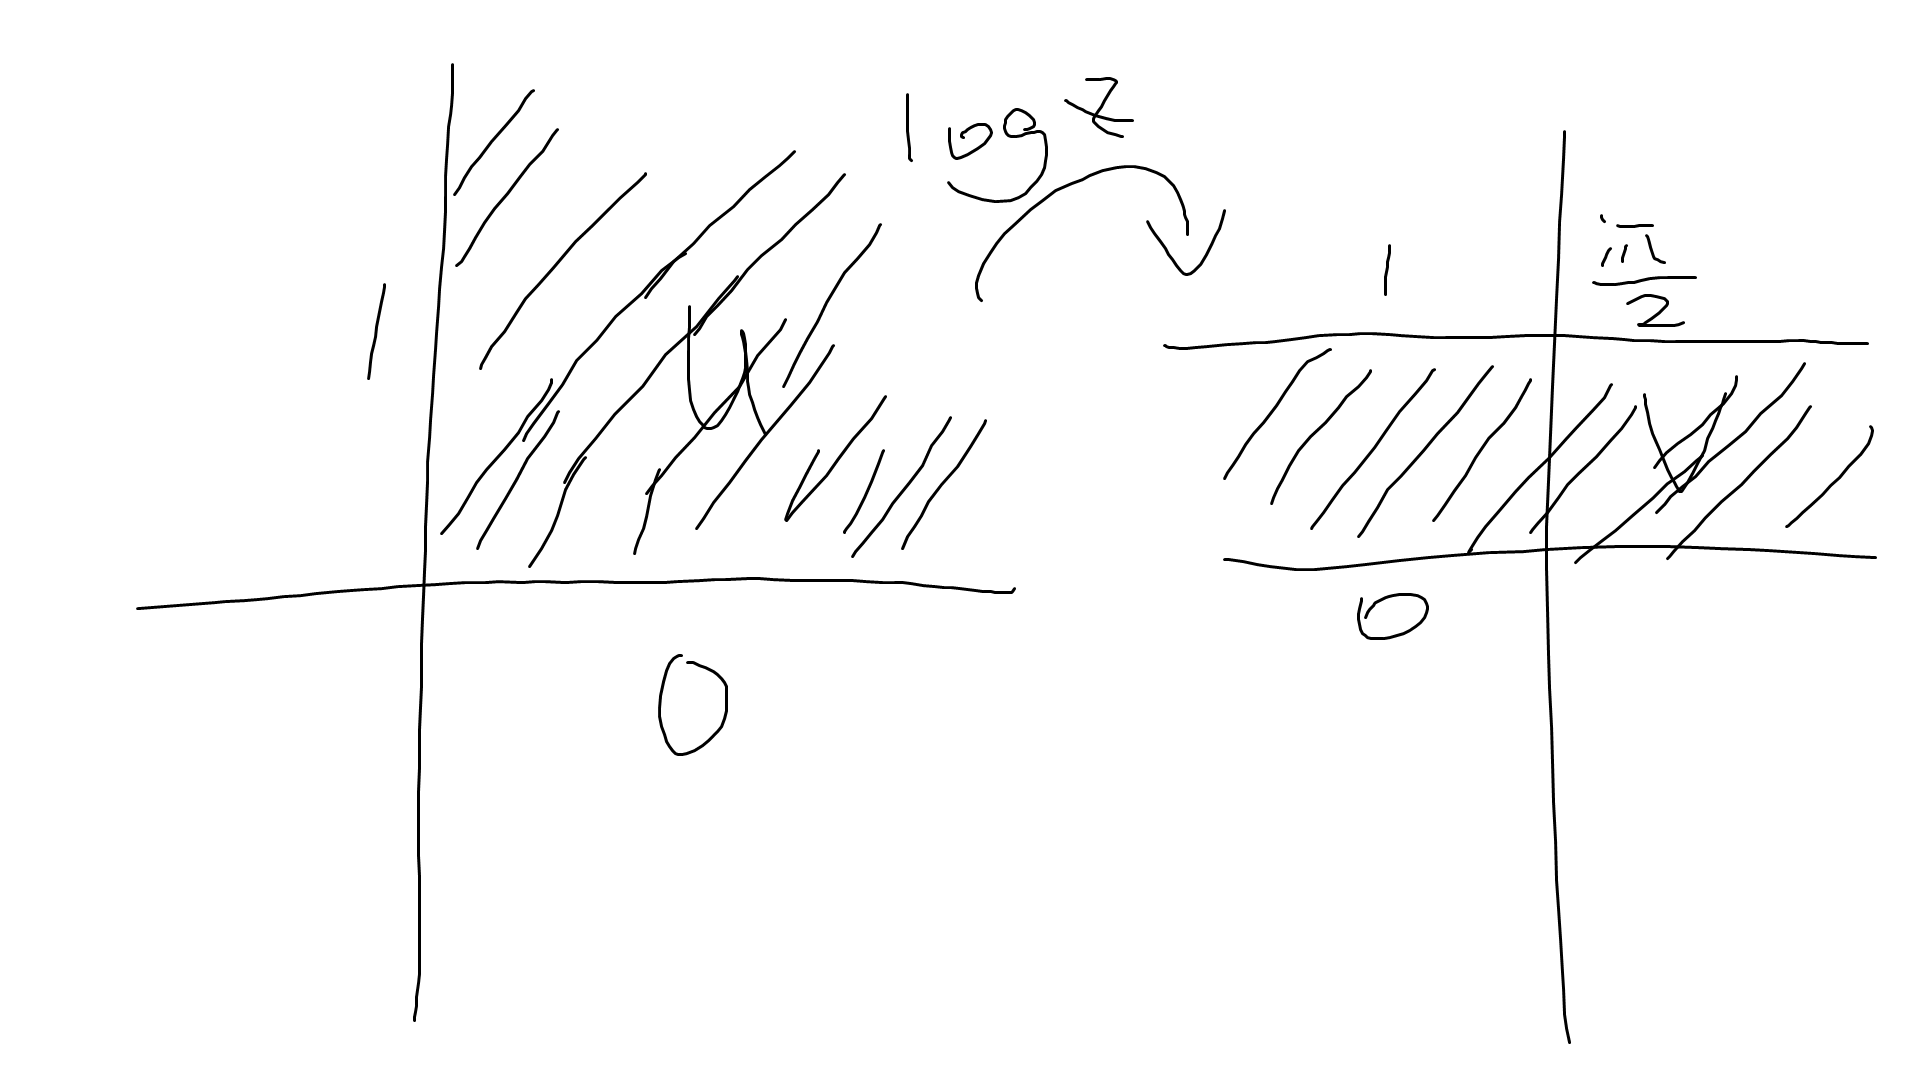
\includegraphics[scale=0.4]{CM_13}

It takes the positive real axis to $\Im z=0$ and the positive imaginary axis to $\Im z = \frac{\pi}{2}$. Therefore we must solve $\nabla^2 \Phi = 0$ in $V$ subject to boundary conditions $\Phi(x,0) = 0$, $\phi(x,\frac{\pi}{2}) = 1$, and $\Phi$ bounded as $x \to \pm \infty$. By inspection the solution is
\begin{equation*}
\begin{aligned}
\Phi(x,y) = \frac{2}{\pi} y.
\end{aligned}
\end{equation*}
So
\begin{equation*}
\begin{aligned}
phi(x,y) &= \Phi(\Re \log z, \Im \log z)\\
&=\frac{2}{\pi} \Im \log z\\
&=\frac{2}{\pi} \tan^{-1}\left(\frac{y}{x}\right).
\end{aligned}
\end{equation*}
\end{eg}

\newpage

\section{Contour Integration and Cauchy's Theorem}
\subsection{Contours and Integrals}

\begin{defi}
A \emph{curve} $\gamma(t)$ is a (continuous) map $\gamma:[0,1] \to \C$.\\
A \emph{closed curve} is one where $\gamma(0) = \gamma(1)$.\\
A \emph{simple curve} is one which does not intersect itself (except at $t=0,1$ in the case of a simple closed curve).\\
A \emph{contour} is a piecewise smooth curve.\\
We shall, in an abuse of notation, often use the symbol $\gamma$ to denote both the map \emph{and} its image, namely the actual curve in $\C$ traversed in a particular direction.\\
The contour $-\gamma$ is the contour $\gamma$ traversed in the opposite direction. Given two contours $\gamma_1$ and $\gamma_2$, with matching end-points, $i.e. \gamma_1(1) = \gamma_2(0)$, $\gamma_1 + \gamma_2$ denotes the two contours joined end to end.\\
The contour integral $\int_\gamma f(z) dz$ is defined to be 
\begin{equation*}
\begin{aligned}
\int_0^1 f(\gamma(t)) \gamma'(t) dt.
\end{aligned}
\end{equation*}
\end{defi}
Alternatively (and equivalently), for a simple contour we dissect it at points $z_0$, $z_1$, ..., $z_N$ on the contour in that order, where $z_0 = \gamma(0)$ and $z_N = \gamma(1)$, and let $\delta z_n = z_{n+1}-z_n$ for $n=0,...,N-1$. Then
\begin{equation*}
\begin{aligned}
\int_\gamma f(z) dz = \lim_{\Delta \to 0} \sum_{n=0}^{N-1} f(z_n) \delta z_n
\end{aligned}
\end{equation*}
where $\Delta = \max_{n=0,...,N-1} |\delta z_n|$ and, as $\Delta \to 0$, $N \to \infty$.

The result of a contour integral between two points in $\C$ \emph{may} depend on the choice of contour.

For example, consider
\begin{equation*}
\begin{aligned}
I_1 = \int_{\gamma_1} \frac{dz}{z},\\
I_2 = \int_{\gamma_2} \frac{dz}{z}
\end{aligned}
\end{equation*}
where in both cases we integrate from $z=-1$ to $z=1$. around a unit circle: $\gamma_1$ above and $\gamma_2$ below the real axis (see diagram below).

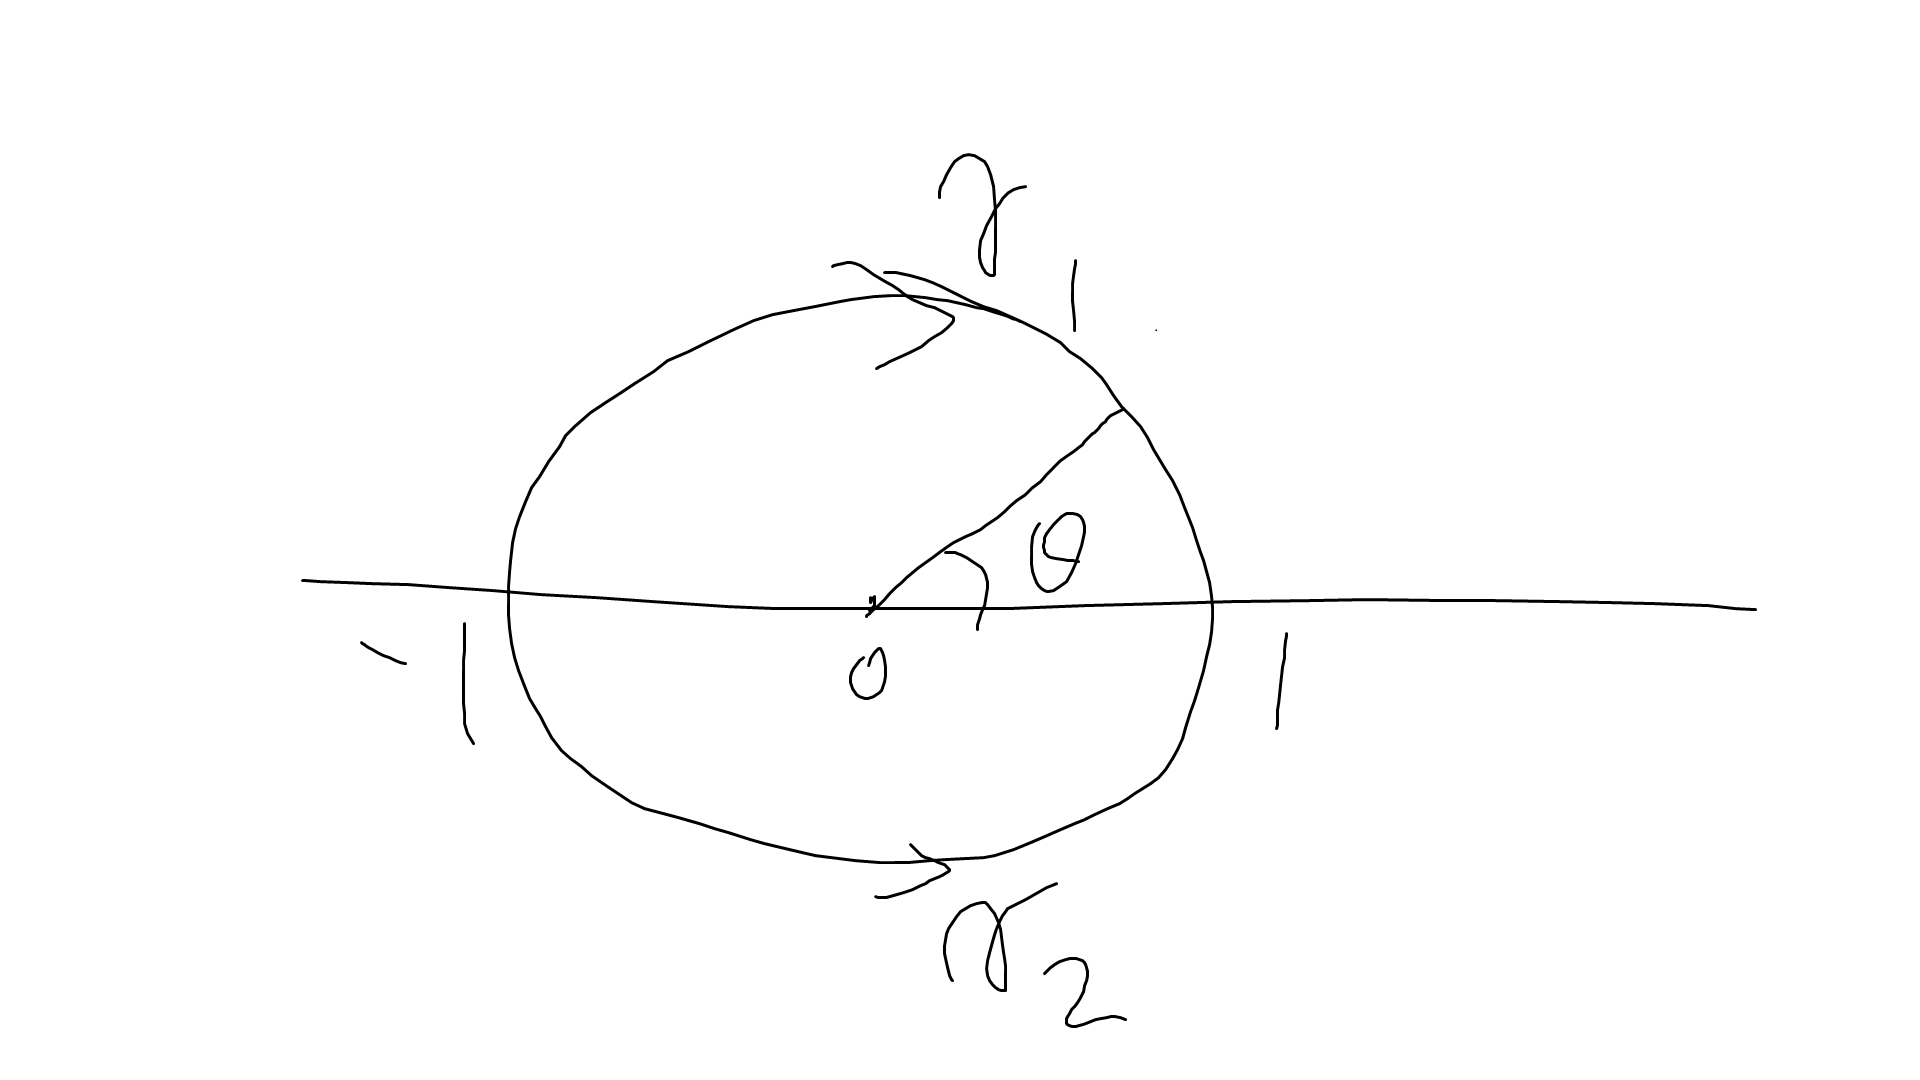
\includegraphics[scale=0.4]{CM_14}

Substitute $z=e^{i\theta}$, then $dz = ie^{i\theta} d\theta$. But then
\begin{equation*}
\begin{aligned}
I_1 = \int_\pi^0 \frac{ie^{i\theta}d\theta}{e^{i\theta}} = -i\pi
\end{aligned}
\end{equation*}
while
\begin{equation*}
\begin{aligned}
I_2 = \int_{-\pi}^0 \frac{ie^{i\theta}d\theta}{e^{i\theta}} = i\pi.
\end{aligned}
\end{equation*}

\subsubsection{Elementary properties}
(i) $\int_{\gamma_1+\gamma_2} f(z) dz = \int_{\gamma_1} f(z) dz + \int_{\gamma_2} f(z) dz$.\\
(ii) $\int_{-\gamma} f(z) dz = -\int_\gamma f(z) dz$.\\
(iii) If $\gamma$ is a contour from $a$ to $b$ in $\C$ then $\int_\gamma f'(z) dz = f(b)-f(a)$ so long as $f$ is differentiable at every point on $\gamma$ (so, for example, we must not cross a branch cut of $f$).\\
(iv) Integration by substitution and by parts work exactly as for integrals on the real line.\\
(v) If $\gamma$ has length $L$ and $|f(z)|$ is bounded by $M$ on $\gamma$, then
\begin{equation*}
\begin{aligned}
|\int_\gamma f(z) dz| \leq LM
\end{aligned}
\end{equation*}
since
\begin{equation*}
\begin{aligned}
|\int_\gamma f(z) dz &\leq \int_\gamma |f(z)| |dz|\\
&\leq M\int_\gamma |dz|\\
&=LM.
\end{aligned}
\end{equation*}

\subsubsection{Integrals on closed contours}
If $\gamma$ is a closed contour, then it doesn't matter where we start from on $\gamma$, as long as we go all the way round.

The notation $\oint f(z) dz$ denotes an integral round a closed contour.

The usual direction of traversal is anticlockwise (the 'positive sense'); if we traverse $\gamma$ in a negative sense (clockwise) then we get the negation of the previous result. More technically, the positive sense is the direction that keeps the interior of the contour on the left.

\subsection{Cauchy's theorem}
If $f(z)$ is analytic in a simply-connected domain $\mathfrak{D}$, then for every simple closed contour $\gamma$ in $\mathfrak{D}$,
\begin{equation*}
\begin{aligned}
\oint_\gamma f(z) dz = 0.
\end{aligned}
\end{equation*}
\begin{proof}(*)\\
The proof of this remarkable theorem is simple and follows from the Cauchy-Riemann equations and Green's Theorem. Let $u,v$ be the real and imaginary parts of $f$. Then
\begin{equation*}
\begin{aligned}
\oint_\gamma f(z) dz &= \oint_\gamma (u+iv)(dx+idy)\\
&= \oint_\gamma (udx - vdy) + i\oint_\gamma (vdx + udy)\\
&= \int_S \left(-\frac{\partial v}{\partial x} - \frac{\partial u}{\partial y}\right) dxdy + i\int_S \left(\frac{\partial u}{\partial x} - \frac{\partial v}{\partial y}\right)dxdy
\end{aligned}
\end{equation*}
where $S$ is the region enclosed by $\gamma$, by applying Green's theorem in the plane,
\begin{equation*}
\begin{aligned}
\oint_{\partial S} (Pdx+Qdy) = \int_S \left(\frac{\partial Q}{\partial x} -\frac{\partial P}{\partial y}\right) dxdy.
\end{aligned}
\end{equation*}
But both brackets vanish by the Cauchy-Riemann equations because $f$ is differentiable throughout $S$. The result follows.
\end{proof}

(**) In fact, this proof requires $u$ and $v$ to have continuous partial derivatives, else Green's theorem isn't applicable. We shall see later that $f$ is in fact differentiable infinitely many times, so $u$ and $v$ do have continuous partial derivatives; unfortunately our proof of that will utilize Cauchy's Theorem. For the complete proof see complex analysis.

\subsection{Contour deformation}
Suppose that $\gamma_1$ and $\gamma_2$ are two contours from $a$ to $b$, and that $f$ is analytic on and between the contours. Then
\begin{equation*}
\begin{aligned}
\int_{\gamma_1} f(z) dz = \int_{\gamma_2} f(z) dz.
\end{aligned}
\end{equation*}
\begin{proof}

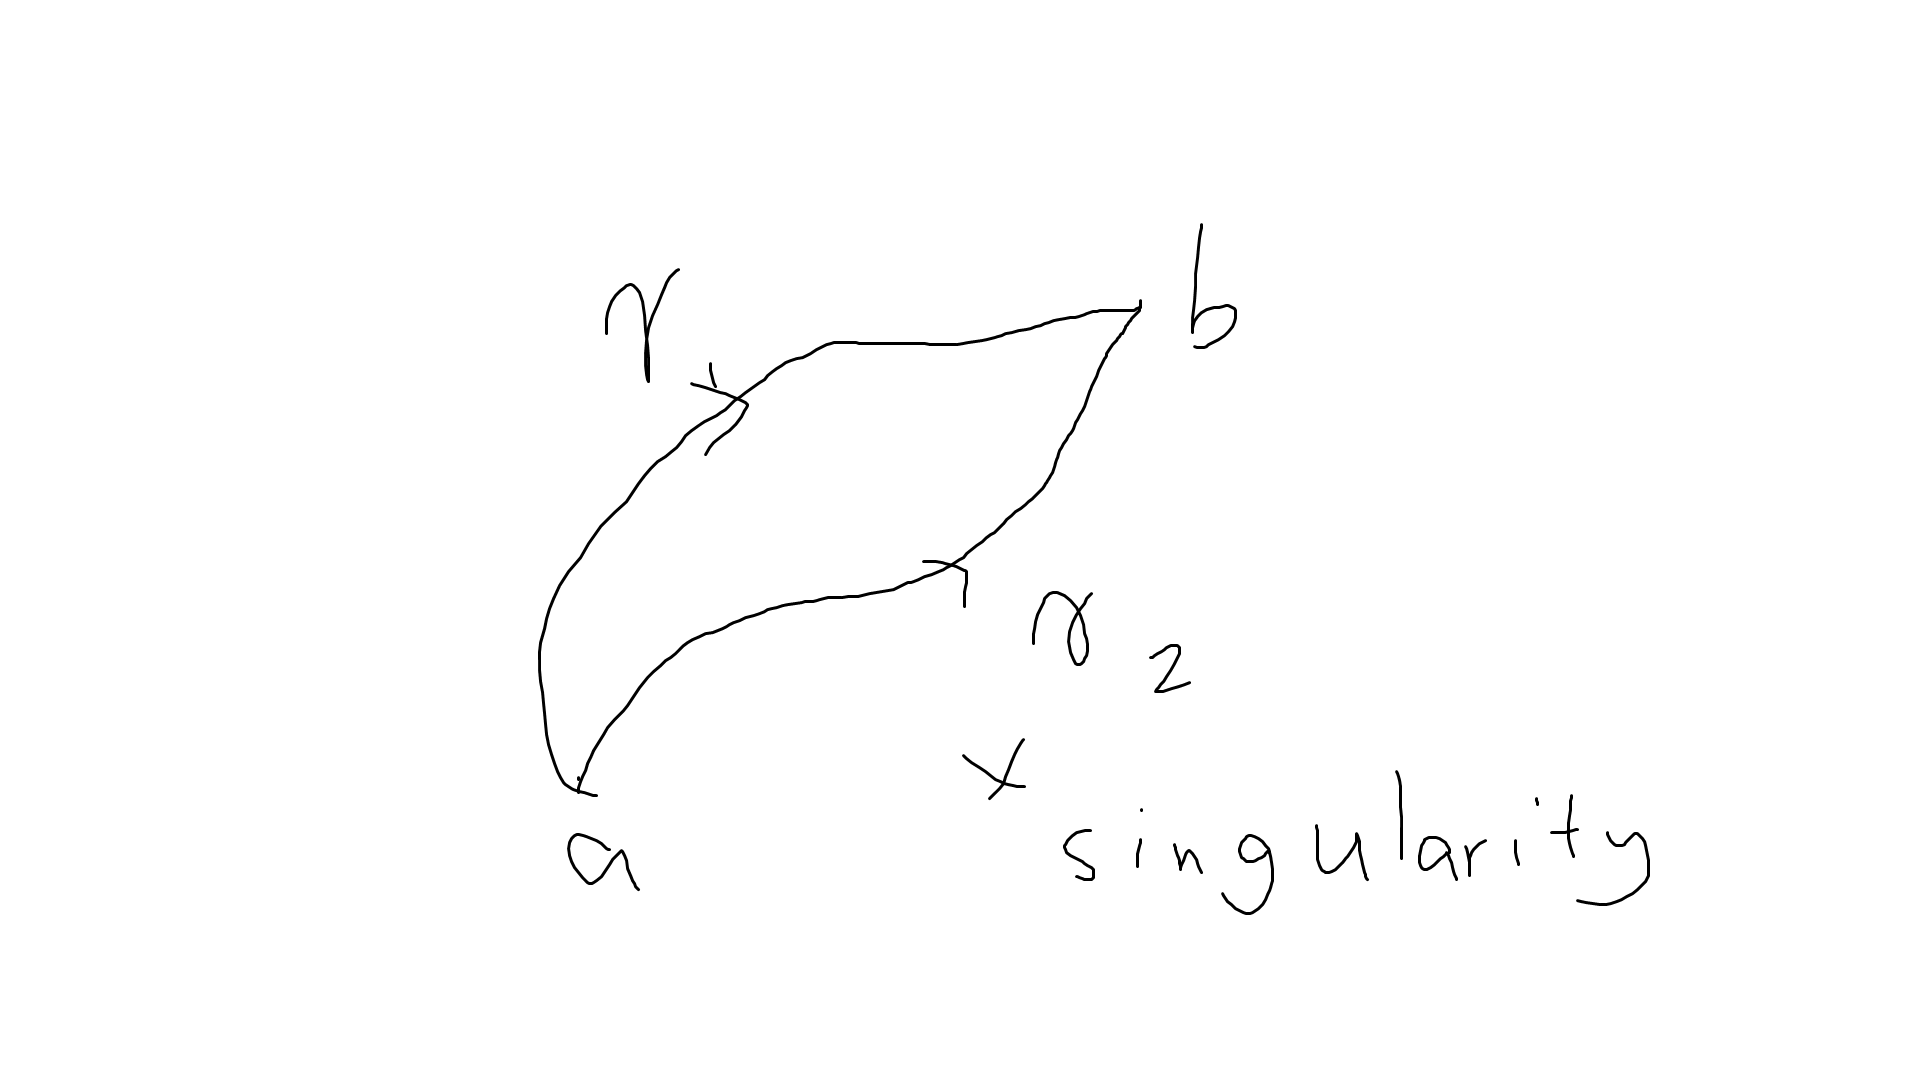
\includegraphics[scale=0.4]{CM_15}

Suppose first that $\gamma_1$ and $\gamma_2$ do not cross. Then $\gamma_1-\gamma_2$ is a simple closed contour, so $\int_{\gamma_1-\gamma_2} f(z) dz = 0$ by Cauchy's Theorem. The result follows.

\end{proof}

If $\gamma_1$ and $\gamma_2$ do cross, then dissect them at each crossing point (e.g. $c$ in the diagram) and apply the technique above to each section.

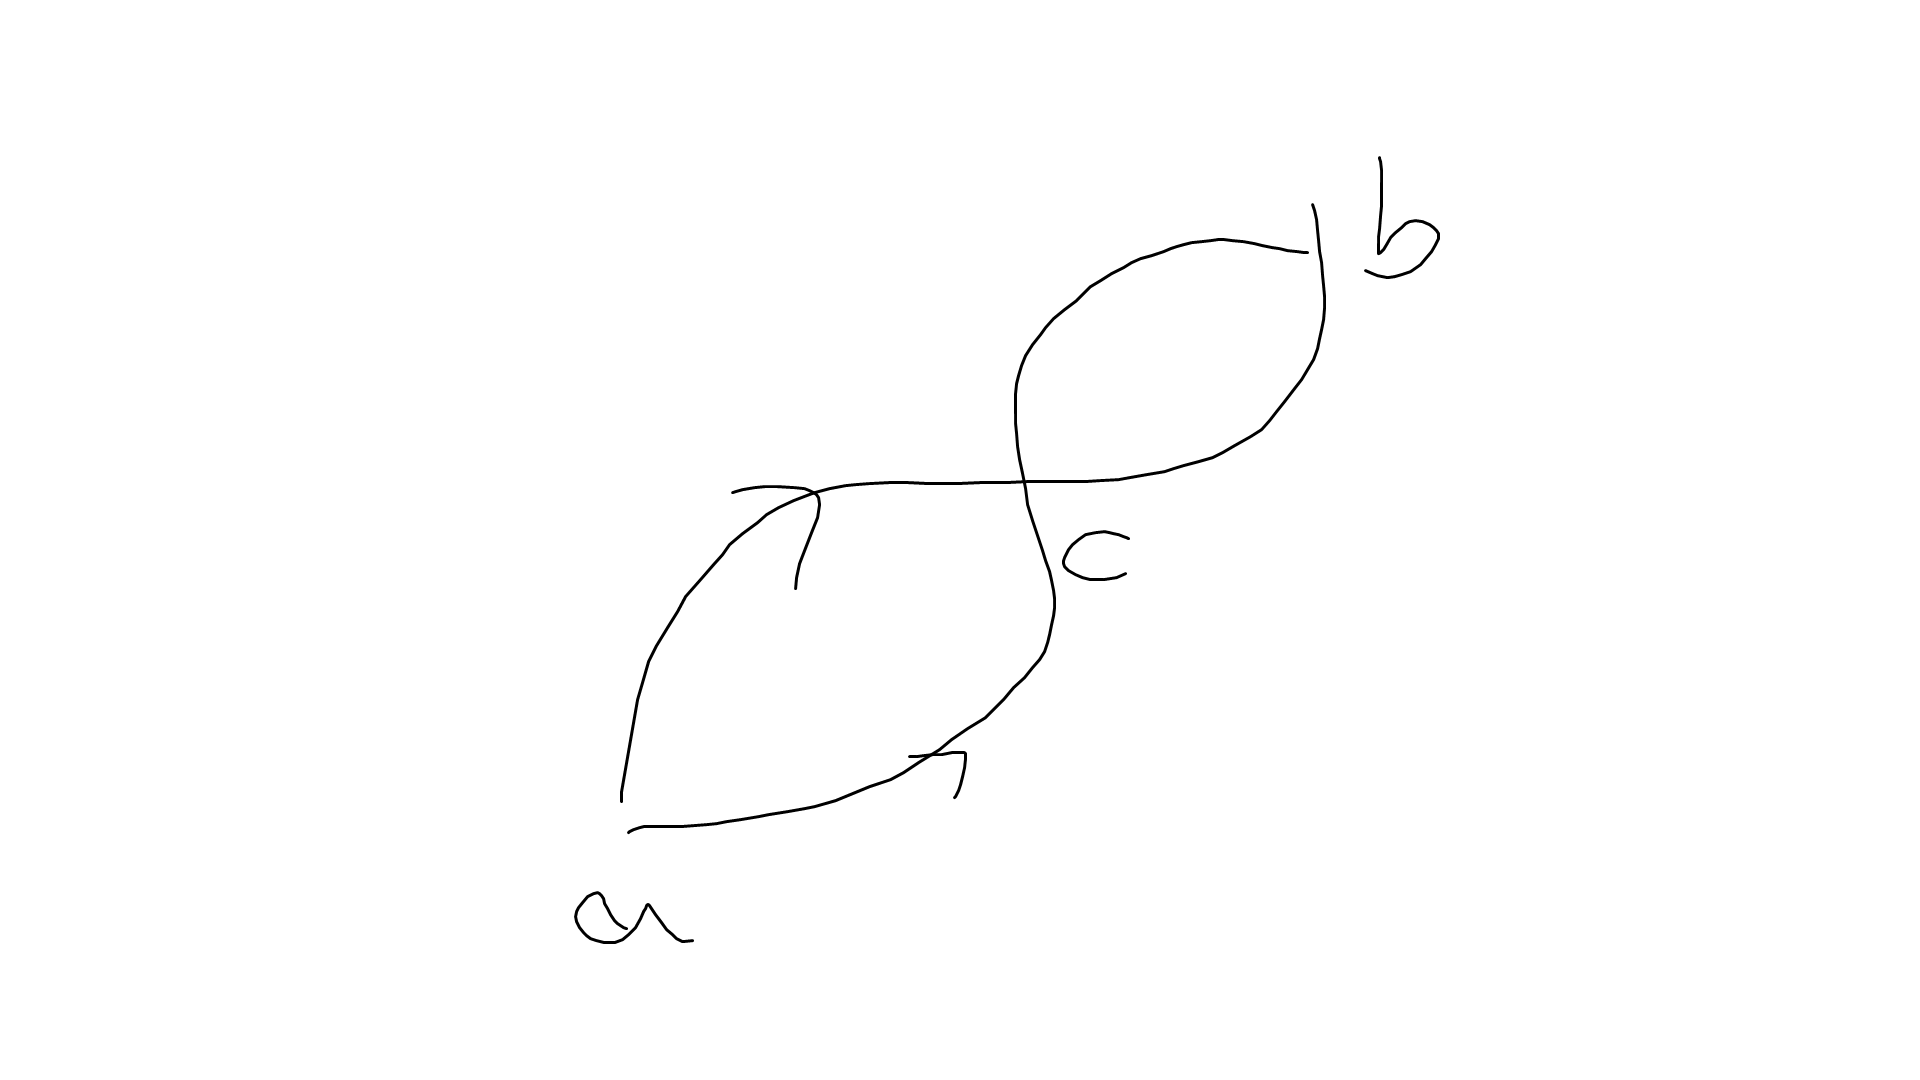
\includegraphics[scale=0.4]{CM_16}

So, if $f$ has no singularities, $\int_a^b f(z) dz$ does not depend on the chosen contour at all.

(*) Another way of thinking about path-independence, and indeed Cauchy's Theorem itself, is to consider $\int f(z)dz$ as a path integral in $\R^2$. Then
\begin{equation*}
\begin{aligned}
f(z)dz &= (u+iv)(dx+idy)\\
&= (u+iv)dx + (-v+iu)dy
\end{aligned}
\end{equation*}
is an exact differential:
\begin{equation*}
\begin{aligned}
\frac{\partial}{\partial y} (u+iv) = \frac{\partial}{\partial x}(-v+iu)
\end{aligned}
\end{equation*}
from the Cauchy-Riemann equations. (*)

The same idea of 'moving the contour' applies to closed contours. Suppose that $\gamma_1$ is a closed contour that can be continuously deformed into another, $\gamma_2$, inside it; and suppose that $f$ has no singularities in the region between them.

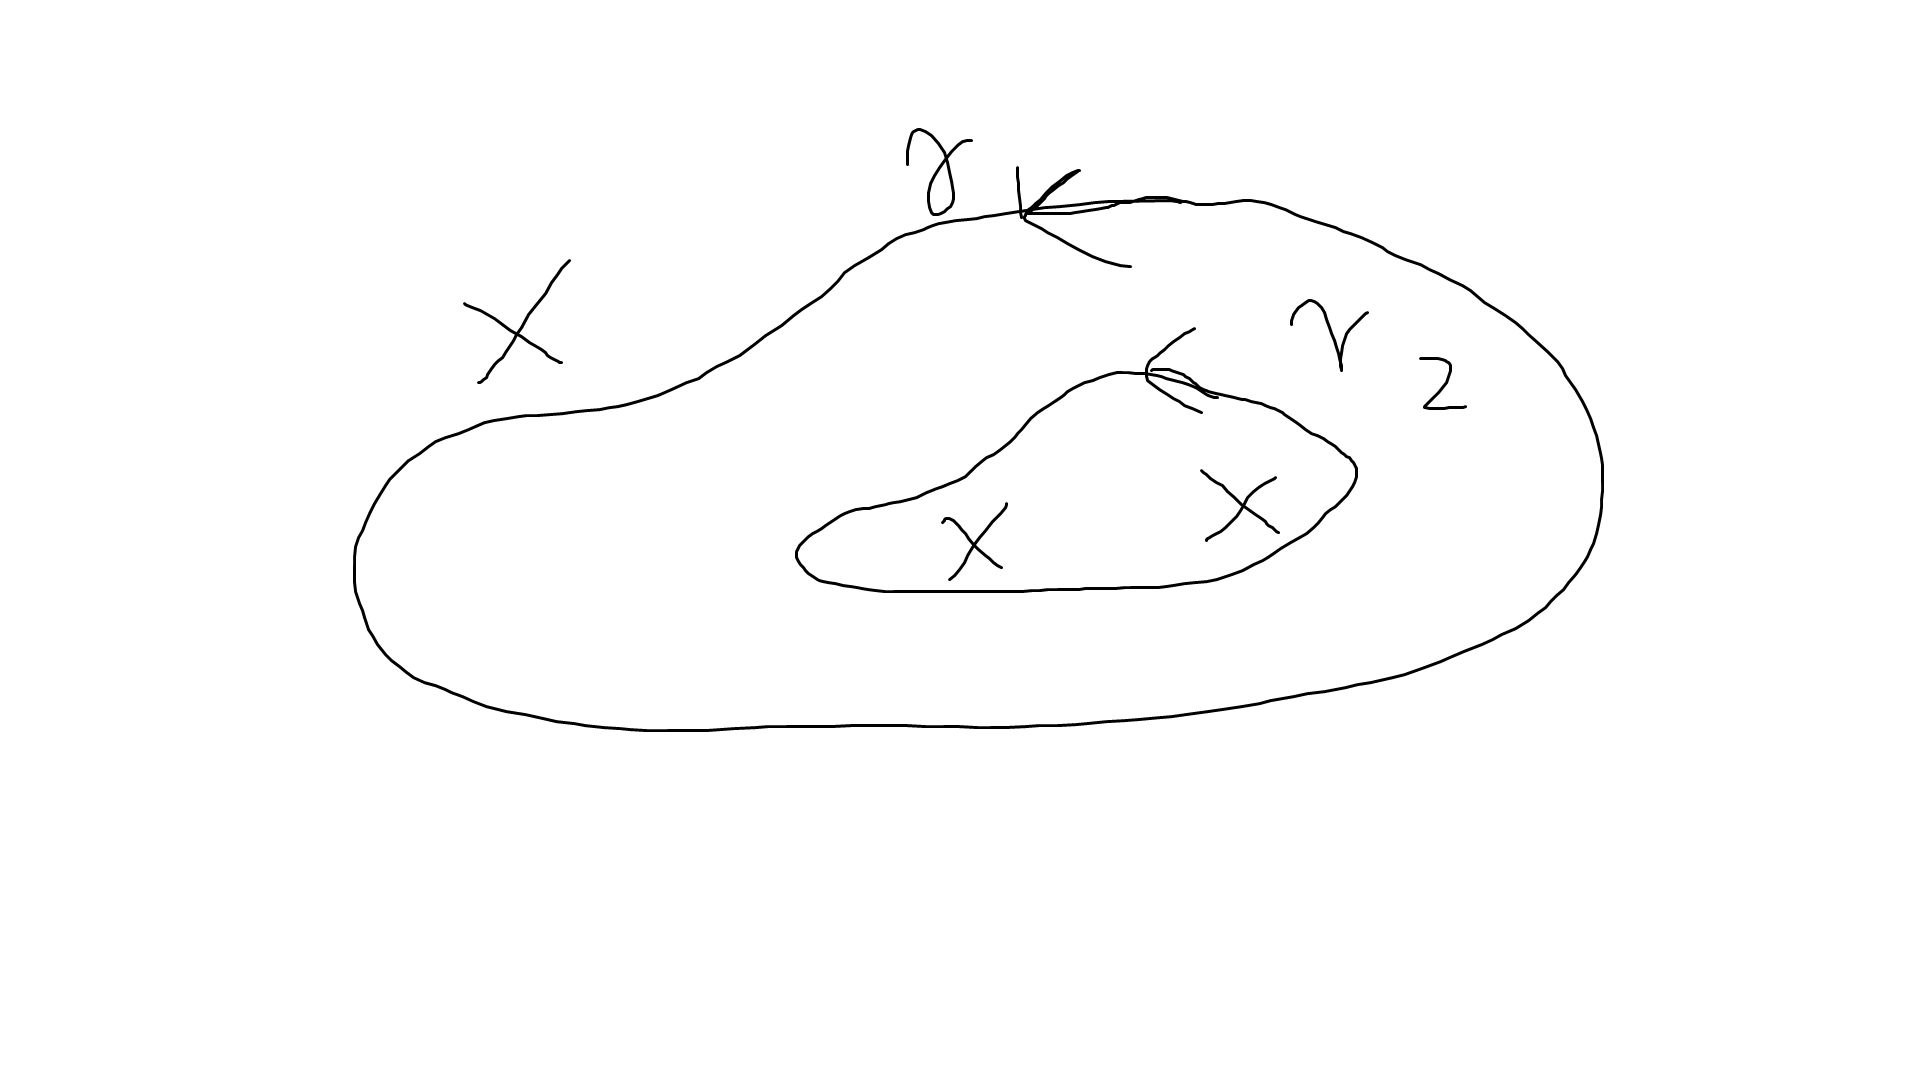
\includegraphics[scale=0.4]{CM_17}

Consider the contour $\gamma$ shown; $\oint_\gamma f(z) dz = 0$.

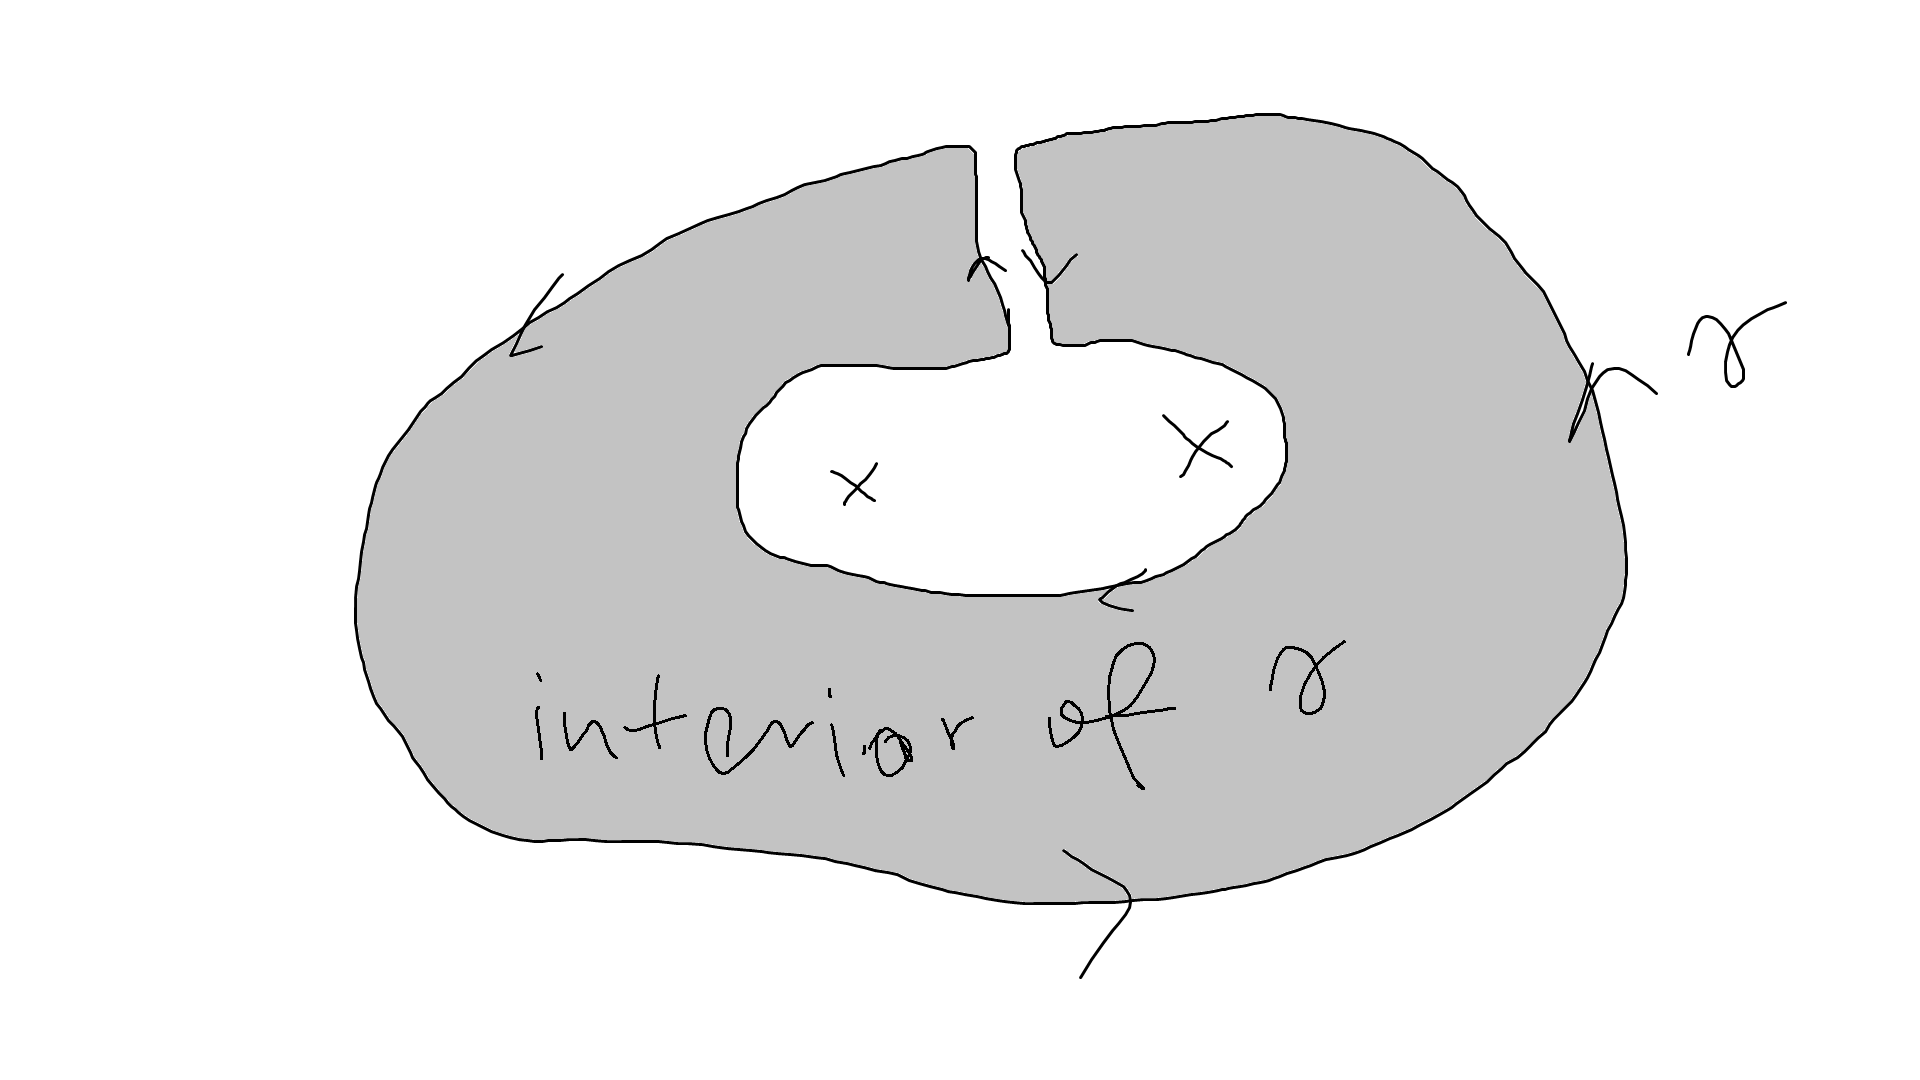
\includegraphics[scale=0.4]{CM_18}

Now let the distance between the two 'cross-cuts' tend to 0; these contributions cancel out and, in the limit, we have
\begin{equation*}
\begin{aligned}
\oint_{\gamma_1} f(z) dz - \oint_{\gamma_2}f(z) dz = 0.
\end{aligned}
\end{equation*}

\subsection{Cauchy's integral formula}
Suppose that $f$ is analytic in a domain $\mathfrak{D}$ and that $z \in \mathfrak{D}$. Then
\begin{equation*} \tag{*}
\begin{aligned}
f(z) = \frac{1}{2\pi i} \oint_\gamma \frac{f(w)}{w-z} dw
\end{aligned}
\end{equation*}
for any simple closed contour $\gamma$ in $\mathfrak{D}$ encircling $z$ anticlockwise. (Note that if $z$ does not lie on or inside $\gamma$ then $\frac{1}{2\pi i} \oint_\gamma \frac{f(w)}{w-z} dw = 0$ by Cauchy's Theorem, since there is no singularity).
\begin{proof} (*)\\
Let $\gamma_\varepsilon$ be a circle of radius $\varepsilon$ about $z$, within $\gamma$.

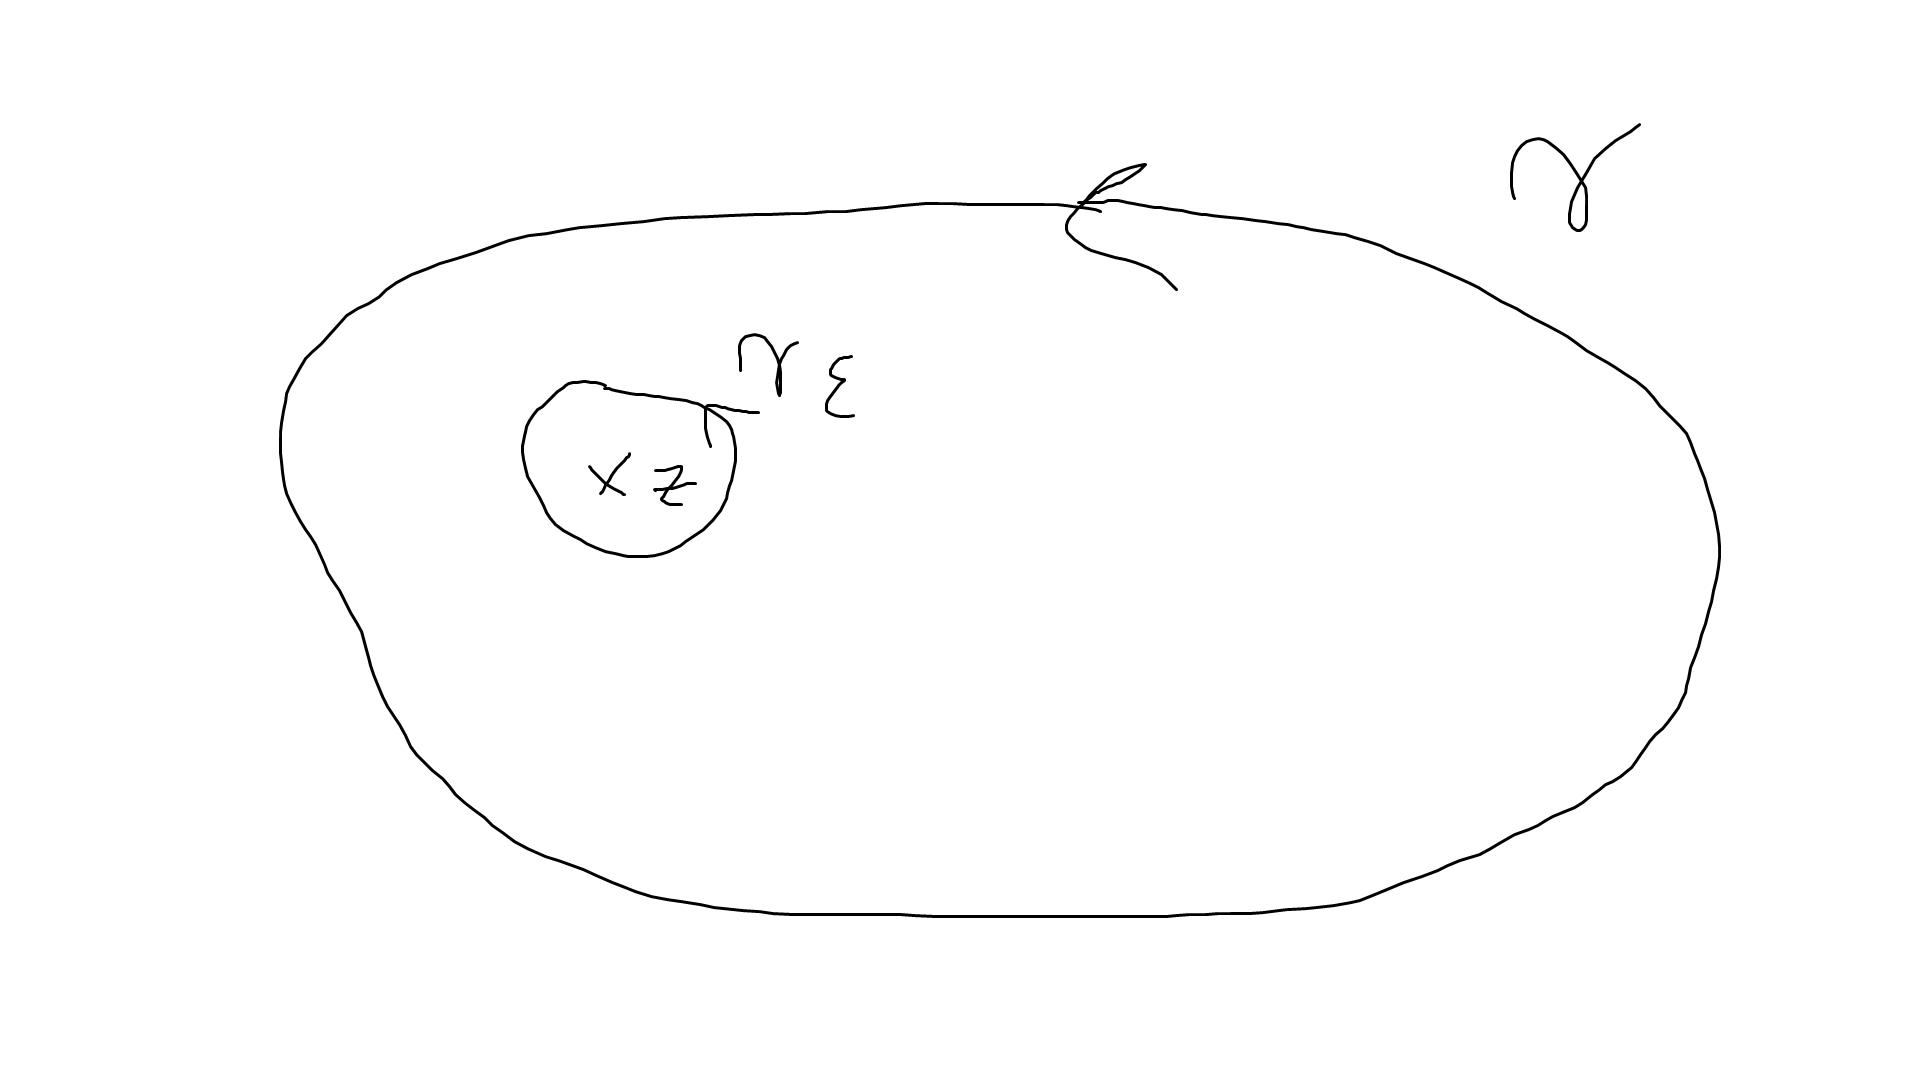
\includegraphics[scale=0.4]{CM_19}

By section 2.3, 
\begin{equation*}
\begin{aligned}
\oint_\gamma \frac{f(w)}{w-z} dw = \oint_{\gamma_\varepsilon} \frac{f(w)}{w-z} dw
\end{aligned}
\end{equation*}
Since the only singularity is at $z$ which is not between $\gamma_\varepsilon$ and $\gamma$. So by substituting $w=z+\varepsilon e^{i\theta}$, the above is then equal to
\begin{equation*}
\begin{aligned}
&\int_0^{2\pi} \frac{f(z+\varepsilon e^{i\theta})}{\varepsilon e^{i\theta}} i\varepsilon e^{i\theta} d\theta\\
= &i \int_0^{2\pi} (f(z)+O(\varepsilon))d\theta\\
\to &2\pi i f(z)
\end{aligned}
\end{equation*}
as $\varepsilon \to 0$. The result follows. (*)

(**) So, if we know $f$ on $\gamma$ then we know it at all points within $\gamma$. Another way of looking at this is to write $f=u+iv$, where $u$ and $v$ are harmonic, and $u,v$ are specified by on $\gamma$; so we have Laplace's equation for $u$ and $v$ with Dirichlet boundary conditions, which has a unique solution inside $\gamma$. (**)

We can differentiate CIF(*):
\begin{equation*}
\begin{aligned}f'(z) = \frac{1}{2\pi i}\oint_\gamma \frac{f(w)}{(w-z)^2} dw
\end{aligned}
\end{equation*}
Differentiation under the integral sign is valid because the integrand, both before and after, is a continuous function of both $w$ and $z$, or in short because this is Complex Methods. Repeating we get
\begin{equation*}
\begin{aligned}
f^{(n)}(z) = \frac{n!}{2\pi i} \oint_\gamma \frac{f(w)}{(w-z)^{n+1}} dw
\end{aligned}
\end{equation*}
Hence at any point where $f$ is analytic, all its derivatives exist, so it is differentiable infinitely many times, as advertised in section 1.2.

(*) An application of Cauchy's integral formula is Liouville's theorem: any bounded entire function is a constant. Suppose that $|f(z)| \leq M$ for all $z$, and consider a circle of radius $r$ centered at an arbitrary $z \in \C$. Then
\begin{equation*}
\begin{aligned}
f'(z) = \frac{1}{2\pi i} \oint_{|w-z|=r} \frac{f(w)}{(w-z)^2} dw
\end{aligned}
\end{equation*}
So from section 2.1(v),
\begin{equation*}
\begin{aligned}
|f'(z)| \leq \frac{1}{2\pi} \cdot 2\pi r \cdot \frac{M}{r^2} = \frac{M}{r}
\end{aligned}
\end{equation*}
which tends to $0$ as $r \to \infty$. Hence $f'(z) = 0$ $\forall z \in \C$. So $f$ is constant, i.e. every bounded entire function is a constant. (*)

(*) Another application is the maximum modulus principle: if $f$ is analytic within a bounded domain and on its boundary, then $|f(z)|$ attains its maximum on the boundary (proof omitted). (*)

\end{proof}

\newpage

\section{Laurent Series and Singularities}
\subsection{Taylor Series}
If $f$ is analytic at $z_0$, then it has a Taylor series 
\begin{equation*}
\begin{aligned}
f(z) = \sum_{n=0}^\infty a_n(z-z_0)^n
\end{aligned}
\end{equation*}
in some neighbourhood of $z_0$ (see section 3.3 for more information about the region of convergence).

All the standard Taylor series from real analysis apply, for example those of $e^z$ and of $(1-z)^{-1}$.

\subsection{Zeros}
The \emph{zeros} of an analytic function $f(z)$ are the points $z_0$ where $f(z_0)=0$. A zero is of \emph{order $N$} if, in its Taylor series, the first non-zero coefficient is $a_N$. Equivalently, it is of order $N$ if
\begin{equation*}
\begin{aligned}
0 = f(z_0) = f'(z_0) = ... = f^{(N-1)} (z_0)
\end{aligned}
\end{equation*}
but $f^(N) (z_0) \neq 0$.

A zero of order one (or two, three, etc) is also called a \emph{simple zero} (or double zero, triple zero etc).

\begin{eg}
$z^3+iz^2+z+i = (z-i)(z+i)^2$ has a simple zero at $z=i$ and a zero of order two at $z=-i$.
\end{eg}

\begin{eg}
$\sinh z$ has zeros where
\begin{equation*}
\begin{aligned}
\frac{e^z - e^{-z}}{2} = 0 \iff e^{2z} = 1 \iff z = n\pi i
\end{aligned}
\end{equation*}
for $n \in \Z$. The zeros are all simple (since $\cosh n\pi i = \cos n\pi \neq 0$).
\end{eg}

\begin{eg}
Since $\sinh z$ has a simple zero at $z= \pi i$, $sinh^3 z$ has a zero of order $3$ there. If needed, we can find its Taylor series about $\pi i$ by writing $\zeta = z-\pi i$:
\begin{equation*}
\begin{aligned}
\sinh^3 z &= [\sinh (\zeta + \pi i)]^3\\
&= [-\sinh \zeta]^3\\
&= -(\zeta + \frac{1}{3!} \zeta^3 + ...)^3\\
&= -\zeta^3 - \frac{1}{2} \zeta^5 - ...\\
&= -(z-\pi i)^3 - \frac{1}{2} (z-\pi i)^5 - ...
\end{aligned}
\end{equation*}
\end{eg}

\subsection{Laurent Series}
If $f$ has a singularity at $z_0$, we cannot expect it to have a Taylor series there. Instead, if $f$ is analytic in an annulus $R_1<|z-z_0|<R_2$, then it has a \emph{Laurent series} about $z_0$,

\begin{equation*}
\begin{aligned}
f(z) = \sum_{n=-\infty}^\infty a_n (z-z_0)^n
\end{aligned}
\end{equation*}
convergent within the annulus (this definition is a bit different from that in GRM).

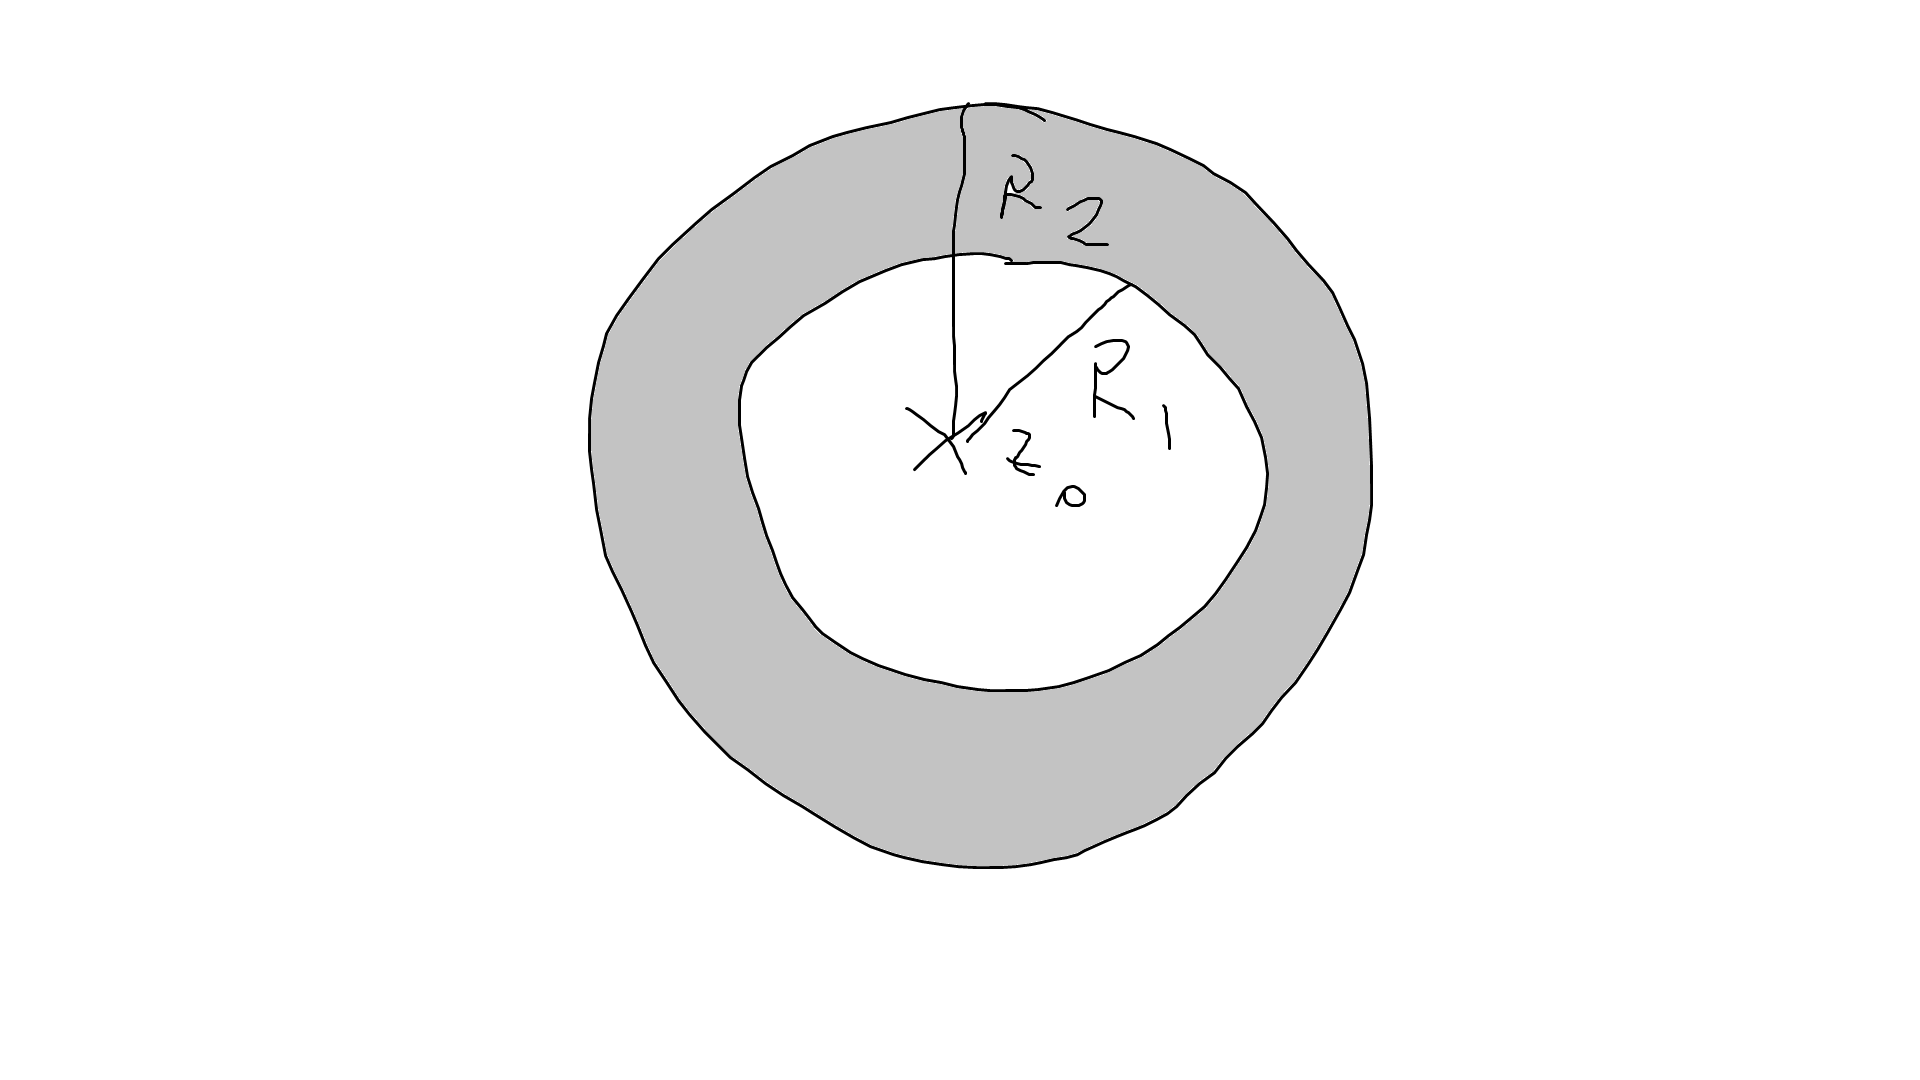
\includegraphics[scale=0.4]{CM_20}

\begin{proof}(*)
See the separate sheet. (*)
\end{proof}

It can be shown that the Laurent Series for $f$ about a particular $z_0$ is unique within any given annulus. Note that Taylor series are just a special case of Laurent Series ($R_1=0$).

\begin{eg}
$\frac{e^z}{z^3}$ has a Laurent series about $z_0=0$ given by
\begin{equation*}
\begin{aligned}
\frac{e^z}{z^3} = \sum_{m=0}^\infty \frac{z^m-3}{m!} = \sum_{n=-3}^\infty \frac{1}{(n+3)!} z^n
\end{aligned}
\end{equation*}
so
\begin{equation*}
\begin{aligned}
a_n = \frac{1}{(n+3)!}
\end{aligned}
\end{equation*}
for $n \geq -3$.
\end{eg}

\begin{eg}
$e^{1/z}$ about $z_0=0$ has
\begin{equation*}
\begin{aligned}
e^{1/z} = 1+\frac{1}{z}+\frac{1}{2!z^2}+\frac{1}{3!z^3}+...,
\end{aligned}
\end{equation*}
so $a_n = \frac{1}{(-n)!}$ for $n\leq 0$.
\end{eg}

\begin{eg}
If $f(z) = \frac{1}{z-a}$ where $a\in \C$, then $f$ is analytic in $|z| < |a|$. So it has a Taylor series about $z_0=0$ given by
\begin{equation*}
\begin{aligned}
\frac{1}{z-a} = -\frac{1}{a}(1-\frac{z}{a})^{-1}= -\sum_{n=0}^\infty a^{-n-1} z^n
\end{aligned}
\end{equation*}
In $|z|>|a|$, it has a Laurent series (in the 'annaulus' $|a|<|z|<\infty$) given by
\begin{equation*}
\begin{aligned}
\frac{1}{z-a} = \frac{1}{z} (1-\frac{a}{z})^{-1} = \sum_{m=0}^\infty \frac{a^m}{z^{m+1}} =\sum_{n=-\infty}^{-1} a^{-n-1}z^n.
\end{aligned}
\end{equation*}
\end{eg}

\begin{eg}
$f(z) = \frac{e^z}{z^2-1}$ has a singularity at $z_0=1$ but is analytic in an annulus $0<|z-z_0|<2$ (since the only other singularity is at $z=-1$). Write everything in terms of $\zeta = z-z_0$, so
\begin{equation*}
\begin{aligned}
f(z) &= \frac{e^{\zeta}e^z_0}{\zeta(\zeta+2)}\\
&=\frac{e^{z_0}}{2\zeta} e^\zeta \left(1+\frac{1}{2}\zeta\right)^{-1}\\
&= \frac{e}{2\zeta} \left(1+\zeta+\frac{1}{2!}\zeta^2+...\right) \left(1-\frac{1}{2}\zeta + \frac{1}{4} \zeta^2-...\right)\\
&= \frac{e}{2\zeta} \left((1+\frac{1}{2}\zeta+\frac{1}{4}\zeta^2+...\right)\\
&=\frac{1}{2} e \left(\frac{1}{z-z_0} + \frac{1}{2} + \frac{z-z_0}{4}+...\right).
\end{aligned}
\end{equation*}
Hence $a_{-1} = \frac{1}{2} e$, $a_0 = \frac{1}{4}e$, etc. This series is valid in the whole annulus (our expansion of $(1+\frac{1}{2}\zeta)^{-1}$ was valid for $|\frac{1}{2}\zeta|<1$, i.e. $|z-z_0|<2$).
\end{eg}

\begin{eg}
The above doesn't seem to work for $f(z) = z^{-1/2}$: we cannot find a Laurent series about $z_0=0$. The reason is that the required branch cut (see section 1.4) would pass through any annulus about the origin, so we cannot find an annulus in which $f$ is analytic (of course, $z^{-1/2}$ has Taylor series about other points $z_0 \neq 0$ except those on the branch cut).
\end{eg}

\subsubsection{Radii of convergence}
Suppose we have a Laurent series that we know to be valid in some annulus $R_1 < |z-z_0| < R_2$ but that there are no singularities on $|z-z_0|=R_2$.

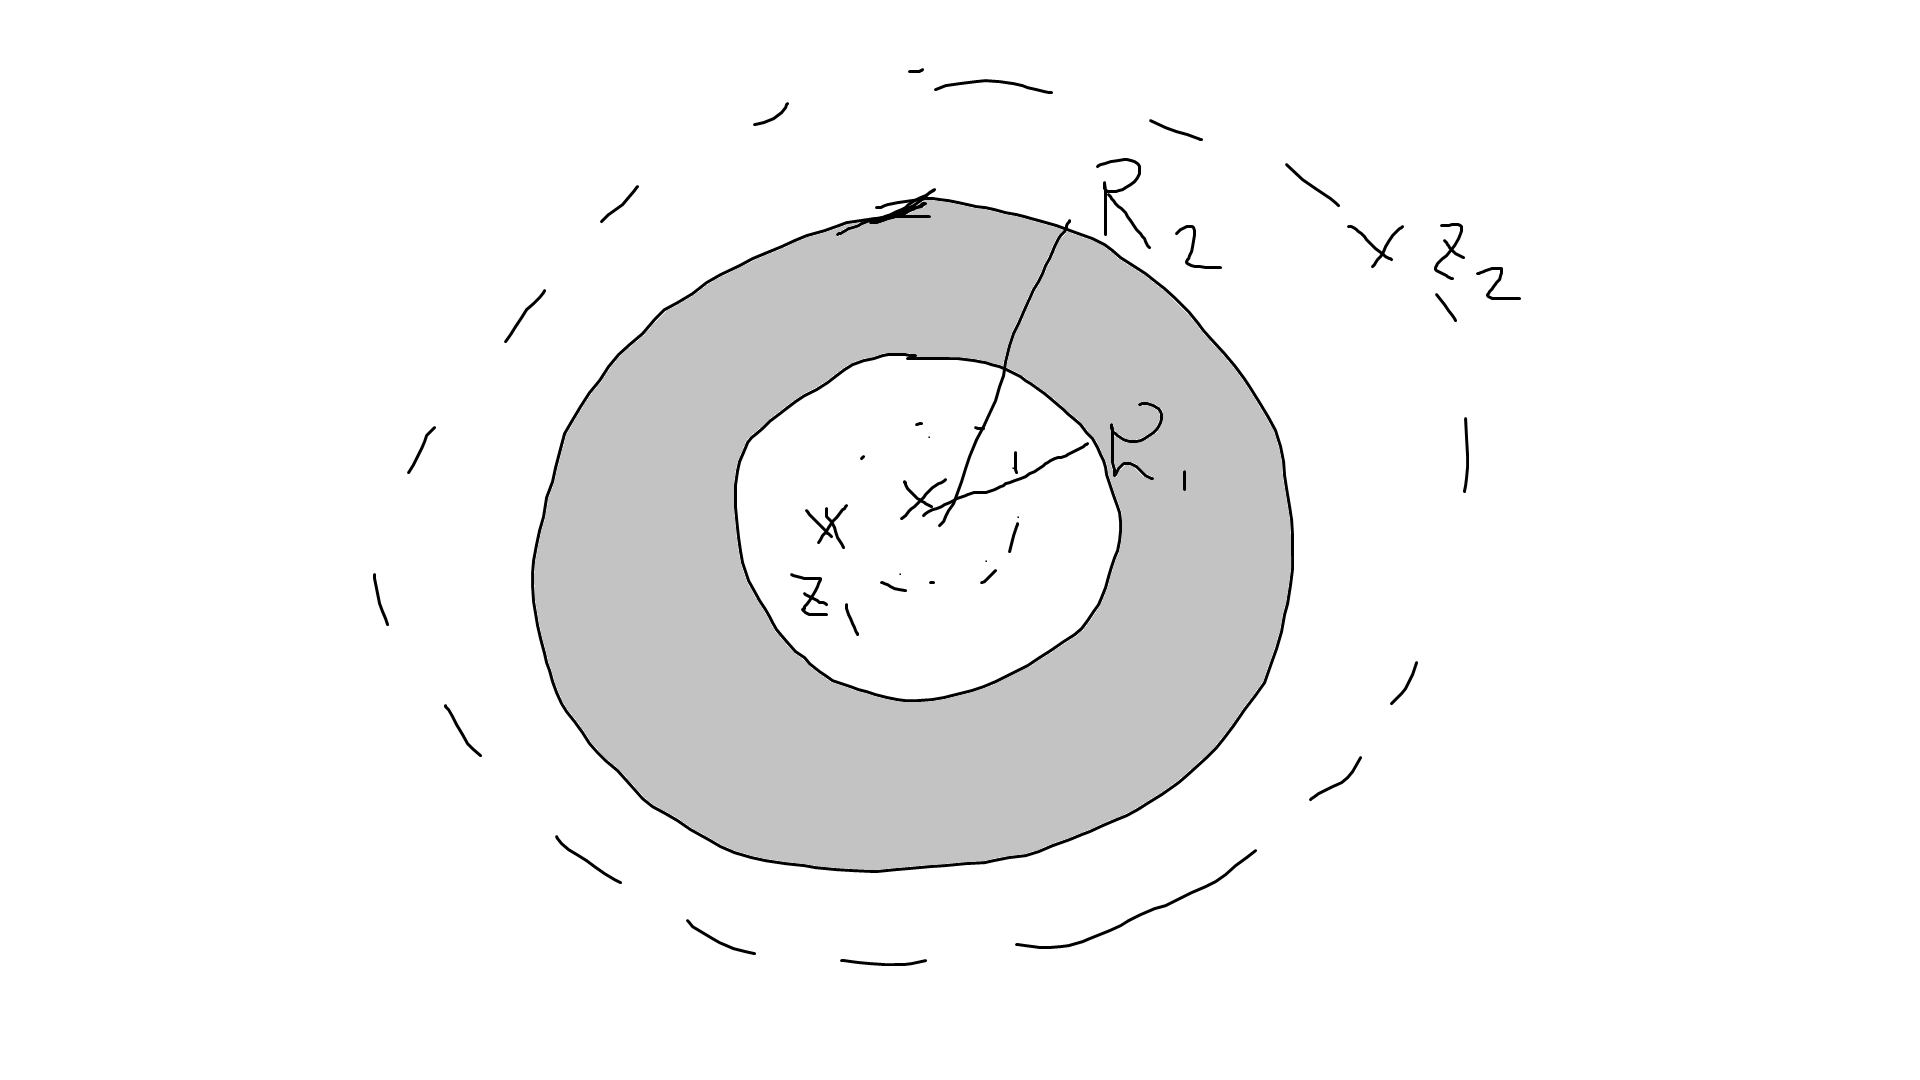
\includegraphics[scale=0.4]{CM_21}

Then the outer radius of convergence can actually be pushed outwards until the circle touches a singularity, say at $z_2$. Similarly, if there are no singularities on $|z-z_0|=R_1$, then the inner radius can be pulled inwards until that circle touches a singularity, say at $z_1$. Then our Laurent series in fact converges in the new annulus
\begin{equation*}
\begin{aligned}
|z_1| \equiv R'_1 < |z-z_0| < R'_2 \equiv |z_2|.
\end{aligned}
\end{equation*}
In other words, the annulus of convergence of a Laurent series can always be made maximally large, with a singularity on each of the bounding circles.

(*) This is because we could have stated with $R'_1$ and $R'_2$ in the first place instead of $R_1$ and $R_2$ in the proof that the Laurent series exists; and Laurent series are unique, so this new one must be the same as our old series. (*)

A Taylor series is just a special case of a Laurent series, resulting in the following statement: the radius of convergence of a Taylor series is always the distance to the nearest singularity.

\begin{eg}
$\cosech z$ has Laurent series
\begin{equation*}
\begin{aligned}
\left(z+\frac{z^3}{3!}+...\right)^{-1} = z^{-1} \left(1-\frac{z^2}{6} + ... \right) = \frac{1}{z} - \frac{z}{6} + ...
\end{aligned}
\end{equation*}
for sufficiently small $z \neq 0$, but it is hard to work out when the binomial expansion is valid. Nevertheless the singularities closest to the origin are at $z=\pm \pi i$, so the annulus of convergence is in fact $0<|z|<\pi$.
\end{eg}

\subsection{Classification of singularities}
Suppose that $f$ has a singularity at $z=z_0$. If there is a neighbourhood of $z_0$ within which $f$ is analytic, except at $z_0$ itself, then $f$ has an \emph{isolated singularity} at $z_0$. If there is no such neighbourhood, then $f$ has a \emph{non-isolated singularity} (some authors call this an 'essential singularity', but that creates confusion with another type described below).

\begin{eg}
$\cosech z$ has isolated singularities at $z=n\pi i$, $n \in \Z$ (from section 3.2 (ii)).
\end{eg}

\begin{eg}
$\cosech \frac{1}{z}$ has isolated singularities at $z=\frac{1}{n\pi i}$, $n\neq 0$, and a non-isolated singularity at $z=0$ (since there are other arbitrarily close singularities).
\end{eg}

\begin{eg}
$\cosech z$ has a non-isolated singularity at $z=\infty$ (see section 1.1).
\end{eg}

\begin{eg}
$z^{-1/2}$ has a branch point singularity at $z=0$ (see section 1.4); this is a type of non-isolated singularity (because $z^{-1/2}$ is not analytic at any point on the branch cut), but is usually treated as a separate type of singularity.
\end{eg}

If $f$ has an isolated singularity at $z_0$, we can find an annulus $0<|z-z_0|<r_0$ say within which $f$ is analytic, and therefore has a Laurent series. This gives us a way to classify singularities:\\
(a) Check for a branch point singularity;\\
(b) Check for a non-isolated singularity;\\
(c) Otherwise, consider the coefficients of the Laurent series $\sum_{n=-\infty}^\infty a_n (z-z_0)^n$:\\
(c1) If $a_n=0$ $\forall n<0$, then $f$ has a \emph{removable singularity} at $z_0$;\\
(c2) If $\exists N>0$ such that $a_n = 0$ $\forall n < -N$, but $a_{-N} \neq 0$ then $f$ has a \emph{pole of order $N$} at $z_0$ (For $N=1,2,...$ this is also called a \emph{simple pole}, \emph{double pole}, etc.).\\
(c3) If there does not exist such an $N$, then $f$ has an \emph{essential isolated singularity} at $z_0$.

The behaviour of $f$ near $z_0$ is as follows:\\
1. At a removable singularity, where
\begin{equation*}
\begin{aligned}
f(z) = a_0 + a_1 (z-z_0)+...
\end{aligned}
\end{equation*}
for $0<|z-z_0|<r_0$, $f(z) \to a_0$ as $z \to z_0$; so an easy way to tell that a singularity is removable is that $f$ has a finite limit. We can 'remove the singularity' by redefining $f(z_0) = a_0 = \lim_{z \to z_0} f(z)$; then $f$ will become analytic at $z_0$.\\
2. At a pole, $|f(z)| \to \infty$ as $z \to z_0$.\\
3. At an essential isolated singularity, $f$ does not tend to any finite or infinite limit. (*) In fact, it can be shown that $f$ takes \emph{all} possible complex values (bar at most one) in any neighbourhood of $z_0$, however small. For example, $e^{1/z}$ takes all values except $0$.(*)

\begin{eg}
(i) $\frac{1}{z-i}$ has a simple pole at $z=i$ (since it is its own Laurent series).\\
(ii) $\frac{\cos z}{z}$ has Laurent series
\begin{equation*}
\begin{aligned}
z^{-1} - \frac{1}{2}z + \frac{1}{24}z^3 - ...
\end{aligned}
\end{equation*}
about the origin, so has a simple pole at $z=0$.\\
(iii) $\frac{z^2}{(z-1)^2(z-i)^3}$ has a double pole at $z=1$ and a triple pole at $z=i$. To show formally that, for instance, there is a double pole at $z=1$, notice first that $\frac{z^2}{(z-i)^3}$ is analytic there, so has a Taylor series
\begin{equation*}
\begin{aligned}
b_0+b_1(z-1)+b_2(z-1)^2+...
\end{aligned}
\end{equation*}
for some $b_n$. Hence
\begin{equation*}
\begin{aligned}
\frac{z^2}{(z-1)^2(z-i)^3} = \frac{b_0}{(z-1)^2} + \frac{b_1}{z-1} + ...
\end{aligned}
\end{equation*}
(iv) If $g(z)$ has a zero of order $N$ at $z=z_0$, then $\frac{1}{g(z)}$ has a pole of order $N$ there (and vice vesa). Hence $\cot z$ has a simple pole at the origin, because $\tan z$ has s simple zero there. To prove the general statement, write $g(z) = (z-z_0)^N G(z)$ for some $G(z)$ with $G(z_0) \neq 0$, and note that $\frac{1}{G(z)}$ has a Taylor series about $z_0$.\\
(v) $z^2$ has a double pole at $\infty$ (see section 1.1).\\
(vi) $e^{1/z}$ has an essential isolated singularity at $z=0$ because all the $a_n$'s are non-zero for $n<0$ (see section 3.3(ii)).\\
(vii) $\sin \frac{1}{z}$ also has an essential singularity at $z=0$ because (using the standard Taylor series for $\sin$) there are non-zero $a_n$ for infinitely many $n<0$.\\
(viii) $f(z) = \frac{e^z-1}{z}$ has a removable singularity at $z=0$, because
\begin{equation*}
\begin{aligned}
f(z)= 1+\frac{1}{2!}z + \frac{1}{3!} z^2 + ...
\end{aligned}
\end{equation*}
By defining $f(0)=1$, we would remove the singularity and obtain an entire function.\\
(ix) $f(z) = \frac{\sin z}{z}$ is not defined at $z=0$ but has a removable singularity there; remove it by setting $f(0) = \lim_{z \to 0} f(z) = 1$.\\
(x) A rational function $f(z) = \frac{P(z)}{Q(z)}$ where $P,Q$ are polynomials has a singularity at any point $z_0$ where $Q$ has a zero; but if $P(z_0)=0$ as well, then the singularity is removable by redefining $f(z) = \frac{P'(z_0)}{Q'(z_0)}$ (assuming that $Q$ has a simple zero).
\end{eg}

\subsection{Closed Contour Integrals of Laurent Series}

Suppose that $f$ is analytic within some annulus, so has a Laurent series
\begin{equation*}
\begin{aligned}
\sum_{n=-\infty}^\infty a_n (z-z_0)^n
\end{aligned}
\end{equation*}
there, and that $\gamma$ is an anticlockwise simple closed contour lying within the annulus.

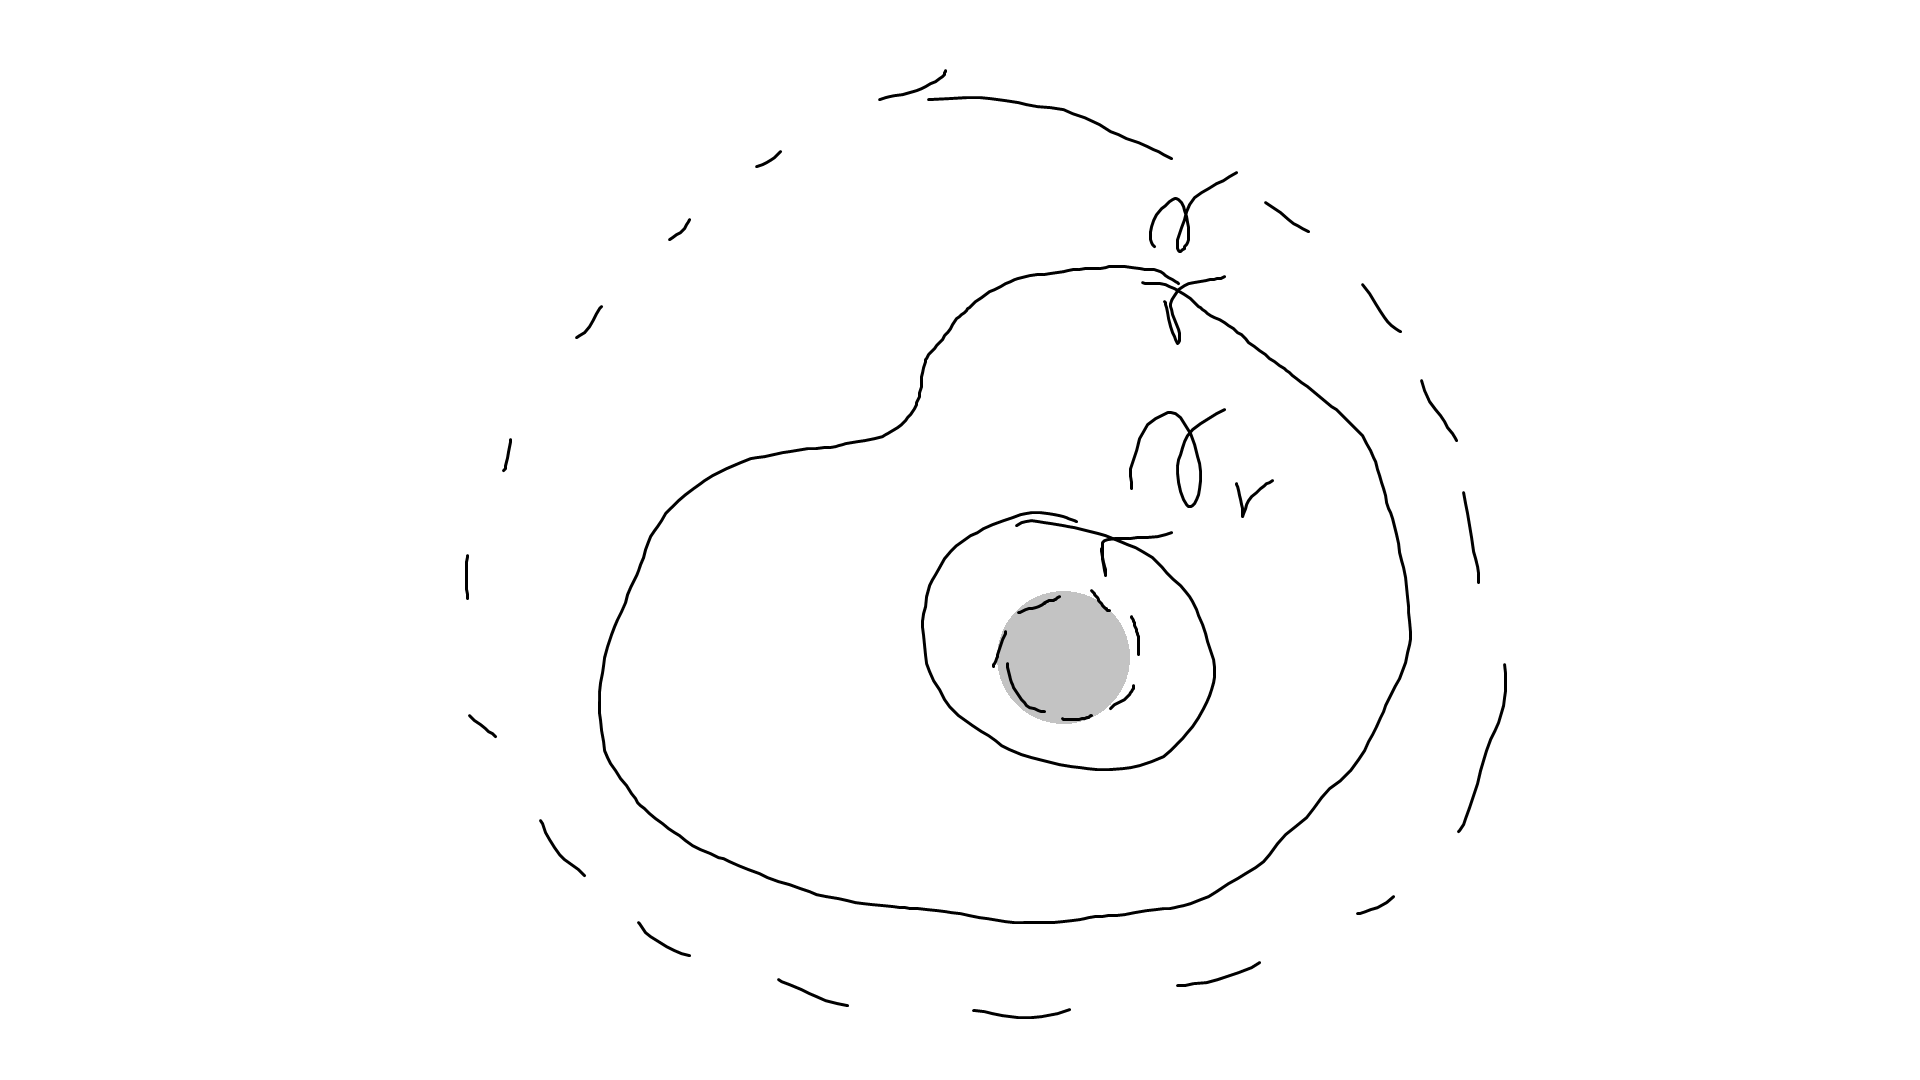
\includegraphics[scale=0.4]{CA_12}

What is $\oint_\gamma f(z) dz$?

Choose a circular contour $\gamma_r$ of radius $r$ lying inside $\gamma$ but still within the annulus. From section 2.3, we can deform the contour, so
\begin{equation*}
\begin{aligned}
\oint_\gamma f(z) dz &= \oint_{\gamma_r} f(z) dz\\
&= \sum_{n=-\infty}^\infty a_n \oint_{\gamma_r} (z-z_0)^n dz
\end{aligned}
\end{equation*}
(by uniform convergence on $\gamma_r$). But let $z=z_0+re^{i\theta}$, then
\begin{equation*}
\begin{aligned}
\oint_{\gamma_r} (z-z_0)^n dz &= \int_0^{2\pi} r^n e^{in\theta} \cdot ire^{i\theta} d\theta\\
&= ir^{n+1} \int_0^{2\pi} e^{i(n+1)\theta} d\theta\\
&= \left\{\begin{array}{ll}
2\pi & n =-1,\\
\frac{r^{n+1}}{n+1} [e^{i(n+1)\theta} ]^{2\pi}_0 = 0 & n \neq -1
\end{array}\right.
\end{aligned}
\end{equation*}
Hence
\begin{equation*}
\begin{aligned}
\oint_\gamma f(z) dz = 2\pi i a_{-1}.
\end{aligned}
\end{equation*}

\newpage

\section{The Calculus of Residues}
\subsection{Residues}
If $f$ has an isolated singularity at $z_0$ then it has a Laurent series expansion about that point (see section 3.4). The \emph{residue} of $f$ at $z_0$ is the coefficient $a_{-1}$ of its Laurent series (we have already seen in section 3.5 that this coefficient is important for evaluating integrals). There is no standard notation but we shall denote the residue by $res_{z=z_0} f(z)$.

At a \emph{simple} pole, the residue is given by
\begin{equation*}
\begin{aligned}
res_{z = z_0} f(z) = \lim_{z \to z_0} \{(z-z_0) f(z)\}
\end{aligned}
\end{equation*}
since the RHS is equal to
\begin{equation*}
\begin{aligned}
\lim_{z \to z_0} \left\{(z-z_0)\left(\frac{a_{-1}}{z-z_0}+a_0+a_1(z-z_0)+...\right)\right\}
\end{aligned}
\end{equation*}
More generally, at a pole of order $N$ the residue is given by
\begin{equation*}
\begin{aligned}
\lim_{z \to z_0} \{\frac{1}{(N-1)!} \frac{d^{N-1}}{dz^{N-1}} ((z-_0)^N f(z)) \}
\end{aligned}
\end{equation*}
which can be proved in a similar manner (see example sheet).

In practice, a variety of techniques can be used to evaluate residues: no single techniques is optimal.

\subsection{The Residue Theorem}
Suppose that $f$ is analytic in a simply-connected domain except at a finite number of isolated singularities $z_1,...,z_n$; and that a simple closed contour $\gamma$ encircles the singularities anticlockwise. 

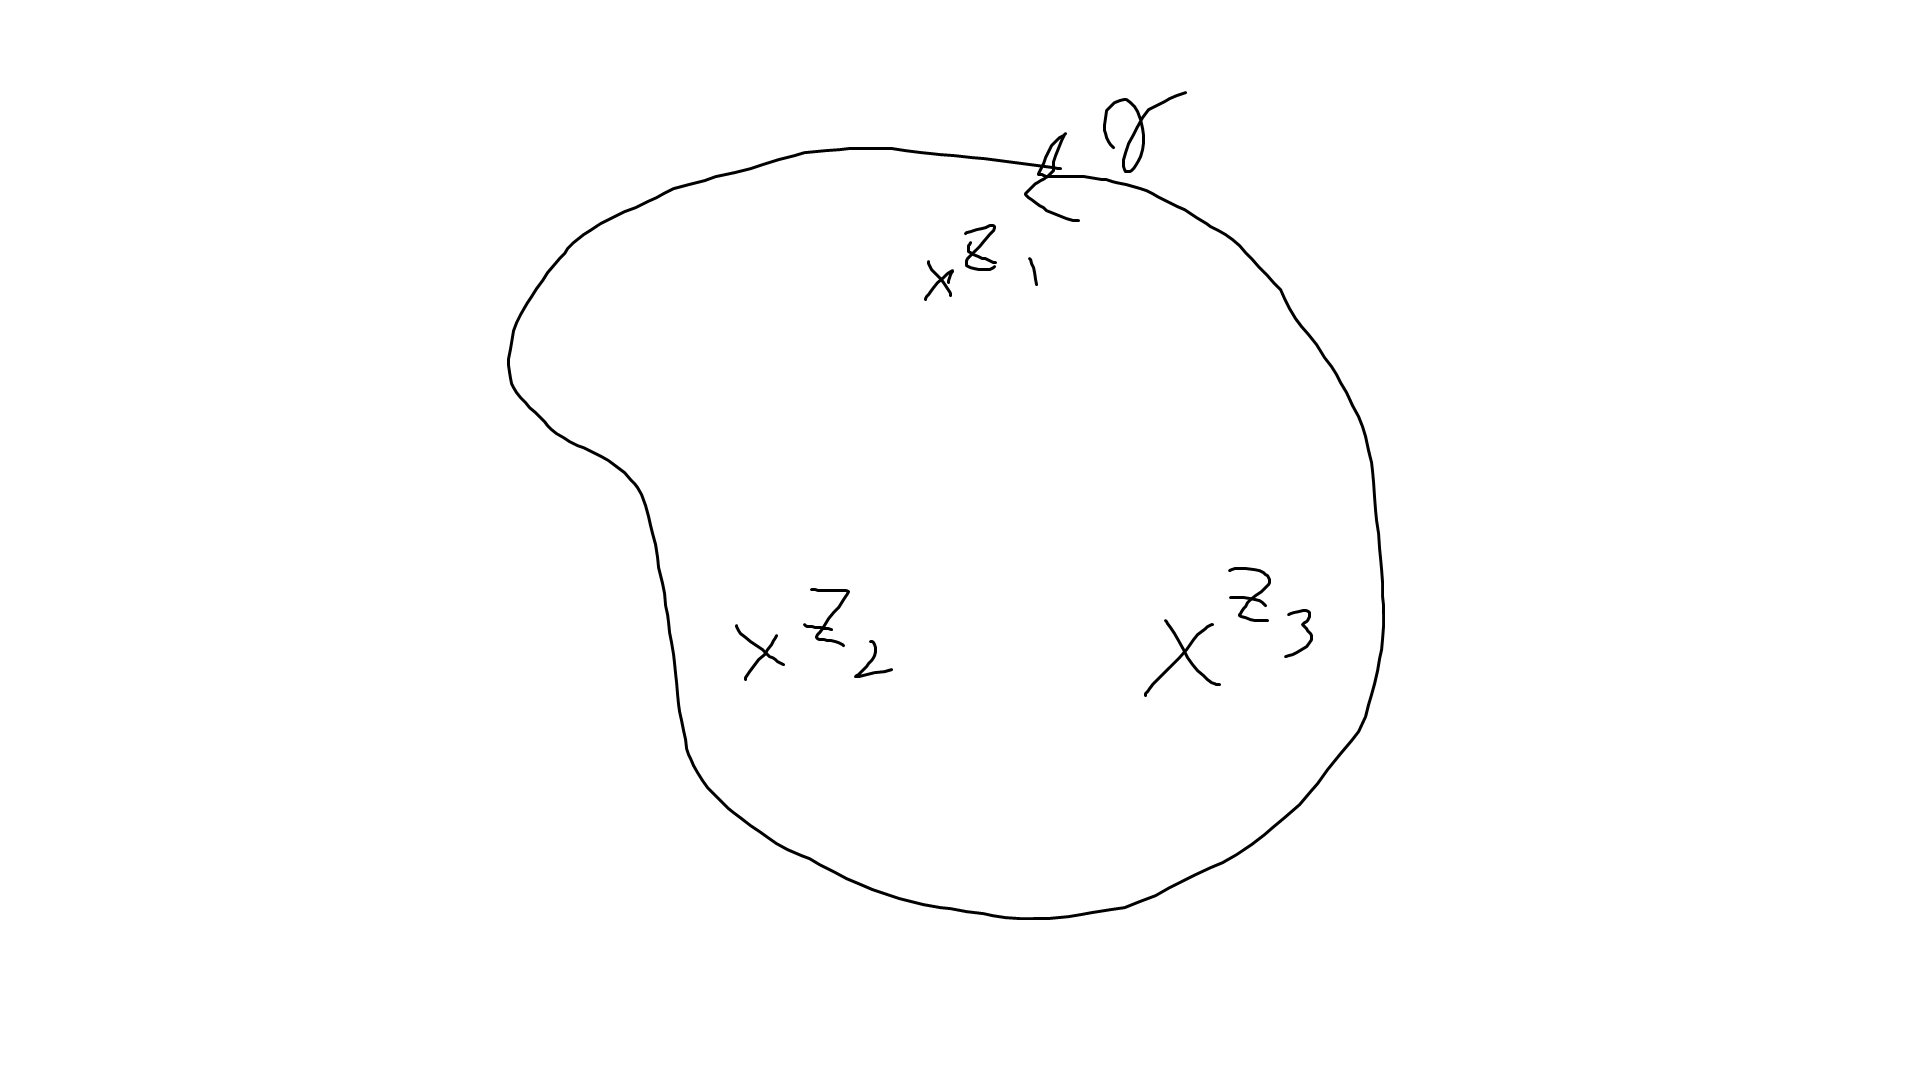
\includegraphics[scale=0.4]{CM_22}

Then
\begin{equation*}
\begin{aligned}
\oint_\gamma f(z) dz = 2\pi i\sum_{k=1}^n res_{z=z_k} f(z).
\end{aligned}
\end{equation*}

\begin{proof}
Consider the curve $\hat{\gamma}$ shown, consisting of small \emph{clockwise} circles $\gamma_1,$...,$\gamma_n$ around the singularities; cross-cuts, which cancel in the limit as they approach each other in pairs, and the large outer curve (which is the same as $\gamma$ in the limit). 

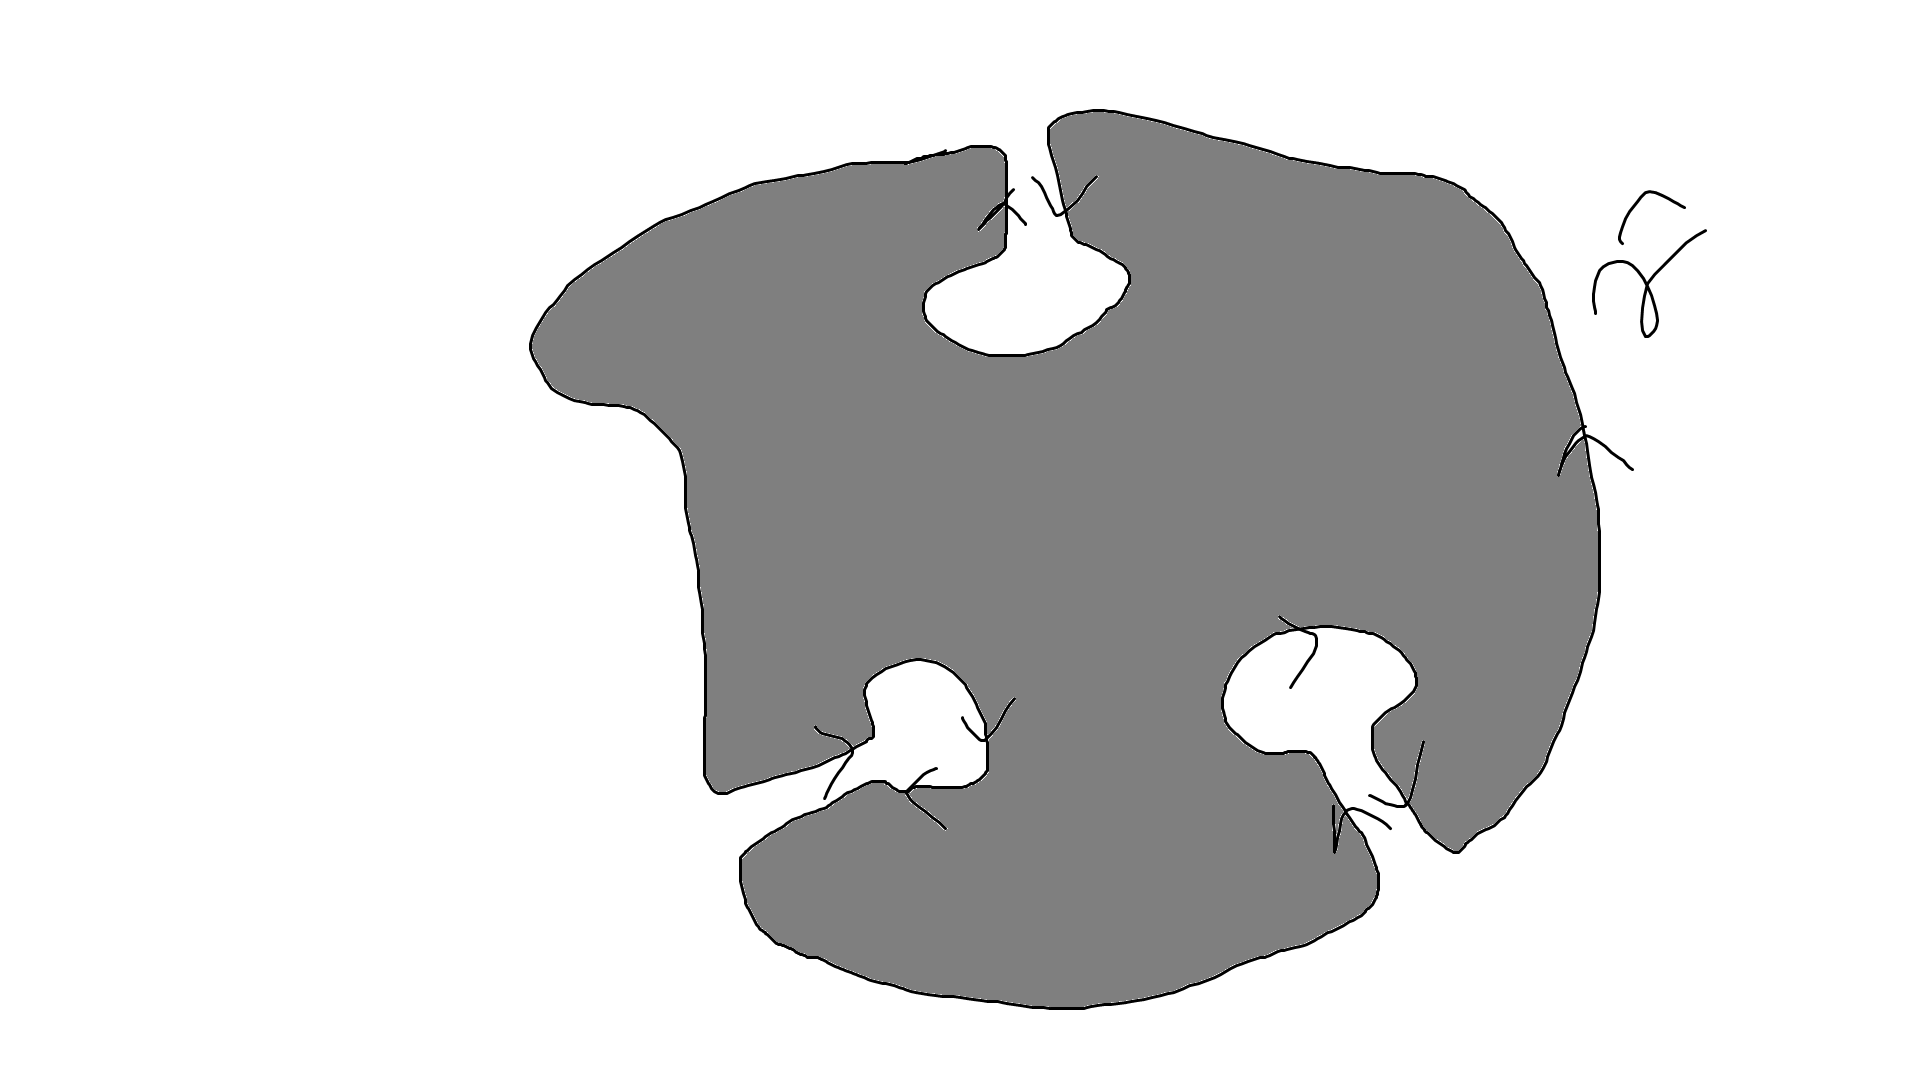
\includegraphics[scale=0.4]{CM_23}

$\hat{\gamma}$ encircles no singularities, so
\begin{equation*}
\begin{aligned}
\oint_{\hat{\gamma}} f(z) dz = 0
\end{aligned}
\end{equation*}
by Cauchy's Theorem. So in the limit when the cross-cuts cancel, we have
\begin{equation*}
\begin{aligned}
\oint_\gamma f(z) dz + \sum_{k=1}^n \oint_{\gamma_k} f(z) dz = \oint_{\hat{\gamma}} f(z) dz = 0
\end{aligned}
\end{equation*}
But about each isolated singularity $z_k$ there is a Laurent series valid locally in some annulus, so by seciont 3.5 and section 4.1 we have
\begin{equation*}
\begin{aligned}
\oint_{\gamma_k} f(z) dz=-2\pi i \ res_{z=z_k} f(z).
\end{aligned}
\end{equation*}
(the minus sign is because $\gamma_k$ is a \emph{clockwise contour}). The result follows.
\end{proof}

\subsection{Applications of the Residue Theorem}
To illustrate the technique we shall evaluate
\begin{equation*}
\begin{aligned}
I = \int_0^\infty \frac{dx}{1+x^2}
\end{aligned}
\end{equation*}
(which we can already do by trigonometric substitutions).

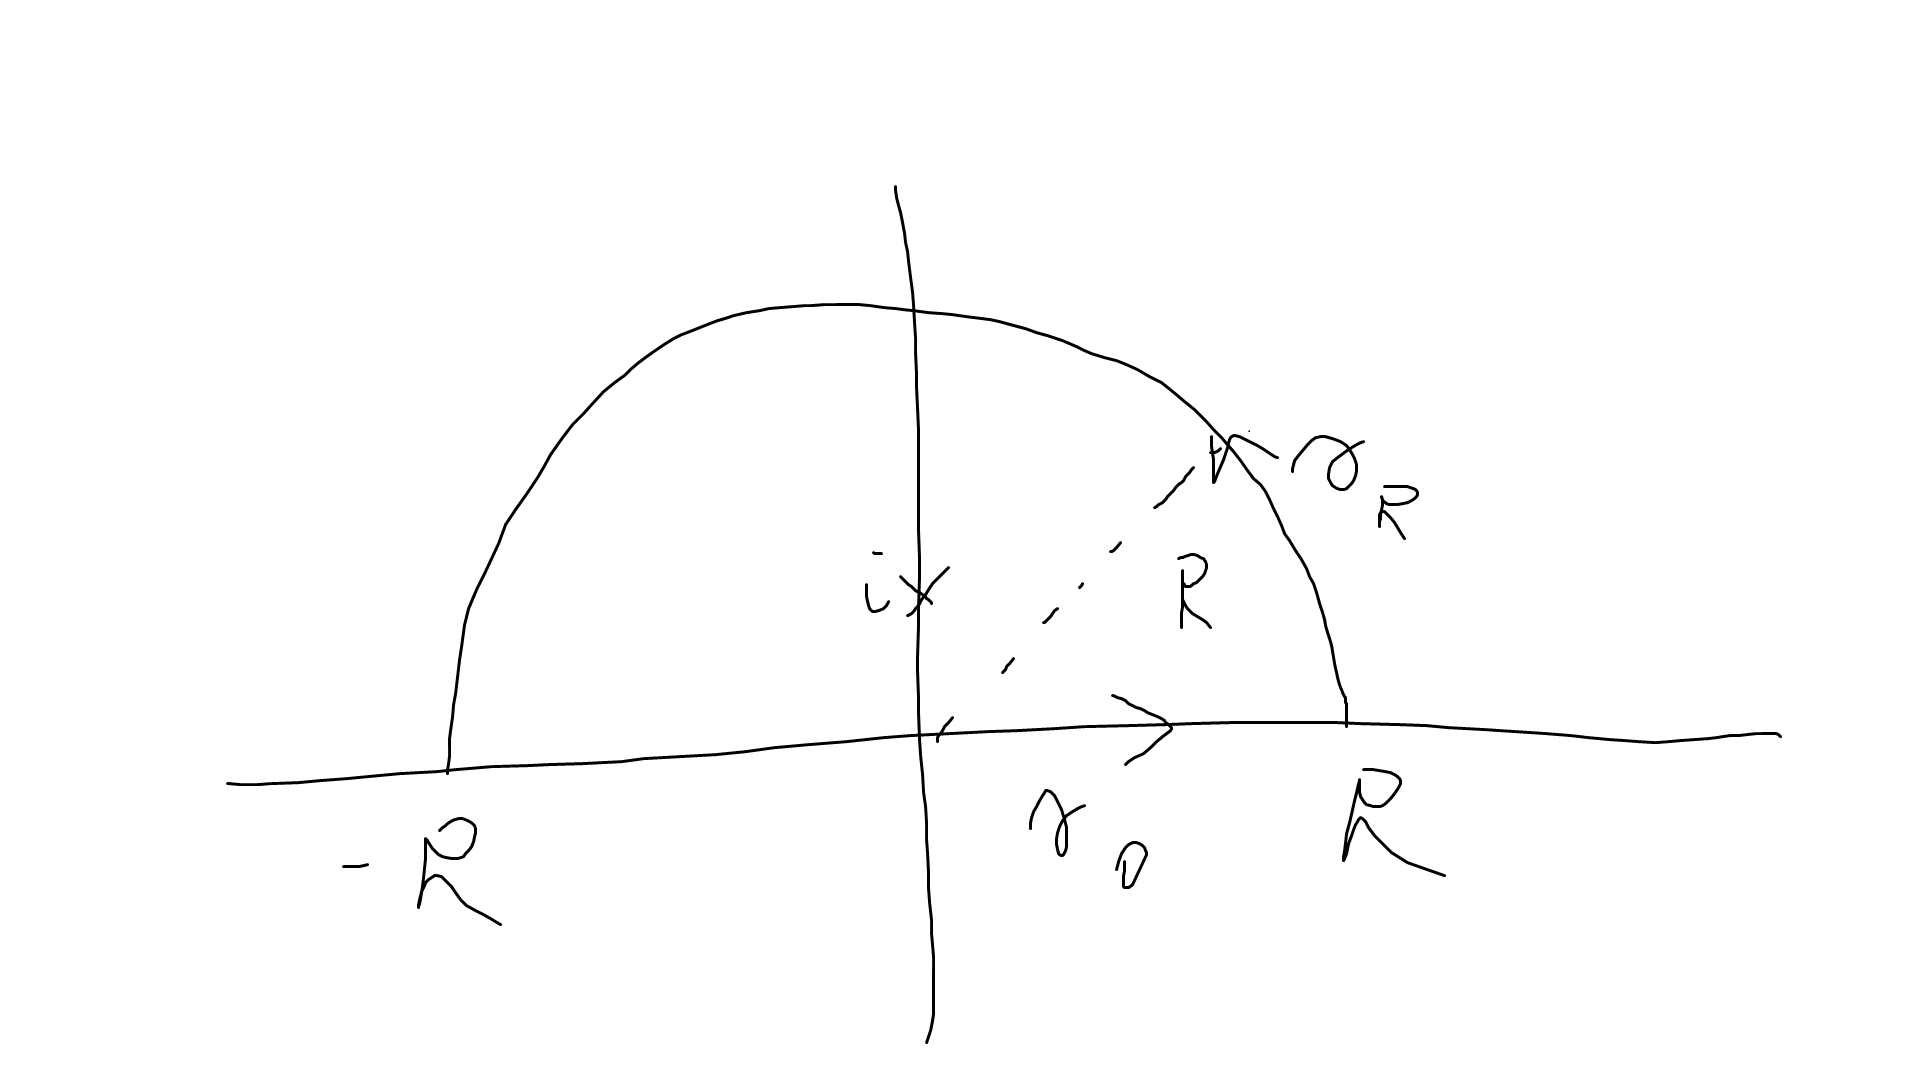
\includegraphics[scale=0.4]{CM_24}

Consider
\begin{equation*}
\begin{aligned}
\oint_\gamma \frac{dz}{1+z^2}
\end{aligned}
\end{equation*}
where $\gamma$ is the contour shown: from $-R$ to $R$ along the real axis ($\gamma_0$) then returning to $-R$ via the upper half plane $\gamma_R$. This is known as 'closing in the upper half plane'. Now
\begin{equation*}
\begin{aligned}
\frac{1}{1+z^2} = \frac{1}{(z+i)(z-i)}
\end{aligned}
\end{equation*}
So the only singularity enclosed by $\gamma$ is a simple pole at $z=i$, where the residue there is
\begin{equation*}
\begin{aligned}
\lim_{z\to i} \frac{1}{z+i} = \frac{1}{2i}
\end{aligned}
\end{equation*}
Hence by the Residue Theorem
\begin{equation*}
\begin{aligned}
\int_{\gamma_0} \frac{dz}{1+z^2} + \int_{\gamma_R} \frac{dz}{1+z^2} &= \oint_\gamma \frac{dz}{1+z^2}\\
&= 2\pi i \frac{1}{2i}\\
&= \pi.
\end{aligned}
\end{equation*}
But 
\begin{equation*}
\begin{aligned}
\int_{\gamma_0} \frac{dz}{1+z^2} = \int_{-R}^R \frac{dx}{1+x^2} \to 2I
\end{aligned}
\end{equation*}
as $R \to \infty$. Also
\begin{equation*}
\begin{aligned}
\int_{\gamma_R} \frac{dz}{1+z^2} \to 0
\end{aligned}
\end{equation*}
as $R \to \infty$ (see below), so we get in the limit
\begin{equation*}
\begin{aligned}
2I + 0 = \pi \implies I = \frac{\pi}{2}.
\end{aligned}
\end{equation*}
To justify $\int_{\gamma_R} \frac{dz}{1+z^2} \to 0$ as $R \to \infty$, we can use a formal or an informal argument:\\
Formal:
\begin{equation*}
\begin{aligned}
|1+z^2| \geq |1-|z|^2| = |1-R^2| = R^2-1
\end{aligned}
\end{equation*}
for large $R$. So
\begin{equation*}
\begin{aligned}
\left|\frac{1}{1+z^2}\right| \leq \frac{1}{R^2-1}.
\end{aligned}
\end{equation*}
From section 2.1(v),
\begin{equation*}
\begin{aligned}
\left| \int_{\gamma_R} \frac{dz}{1+z^2} \right| \leq \pi R \cdot \frac{1}{R^1-1} \to 0
\end{aligned}
\end{equation*}
as $R \to \infty$.

Informal:
\begin{equation*}
\begin{aligned}
\left|\int_{\gamma_R} \frac{dz}{1+z^2}\right| &\leq \pi R \sup_{z \in \gamma_R} \left|\frac{1}{1+z^2}\right|\\
&= \pi R O(R^{-2})\\
&= O(R^{-1}) \to 0
\end{aligned}
\end{equation*}
as $R \to \infty$.

This example is not in itself impressive, but the method adapts easily to more difficult integrals.

Note that we could also have 'closed in the lower half plane' instead. Most of the argument would be unchanged; the residue would now be $res{z=-i} \frac{1}{1+z^2} = -\frac{1}{2i}$, but the contour now goes clockwise, which results in an additional minus sign that cancels each other.

\begin{eg}
To find
\begin{equation*}
\begin{aligned}
I = \int_0^\infty \frac{dx}{(x^2+a^2)^2}
\end{aligned}
\end{equation*}
where $a>0$ is a real constant, consider
\begin{equation*}
\begin{aligned}
\oint_\gamma \frac{dz}{(z^2+a^2)^2}
\end{aligned}
\end{equation*}
where $\gamma$ is as above. The only singularity within $\gamma$ is a pole of order $2$ at $z=ia$, at which the residue is
\begin{equation*}
\begin{aligned}
\lim_{z \to ia} \frac{d}{dz} \frac{1}{(z+ia)^2} &= \lim_{z \to ia}\frac{2}{(z+ia)^3} \\
&= -\frac{1}{4} ia^{-3}
\end{aligned}
\end{equation*}
The integral around $\gamma_R$ still vanishes as $R \to \infty$, since now
\begin{equation*}
\begin{aligned}
\left|\int_{\gamma_R} \frac{dz}{(z^2+a^2)^2}\right| \leq \pi R \cdot  O(R^{-4}) = O(R^{-3}).
\end{aligned}
\end{equation*}
Therefore
\begin{equation*}
\begin{aligned}
2I = 2\pi i (-\frac{1}{4} ia^{-3})
\end{aligned}
\end{equation*}
i.e. $I=\frac{\pi}{4a^3}$.
\end{eg}

\subsection{Advanced Applications of the Residue Theorem: using rectangular contours}

\subsection{Jordan's Lemma}

\newpage

\section{Transform Theory}
\subsection{Fourier Transforms}
The Fourier transforms of a function $f(x)$ that decays sufficiently rapidly as $|x| \to \infty$ is
\begin{equation*}
\begin{aligned}
\tilde{f}(k) \int_{-\infty}^\infty f(x) e^{-ikx} dx
\end{aligned}
\end{equation*}
and the inverse transform is
\begin{equation*}
\begin{aligned}
f(x) = \frac{1}{2\pi} \int_{-\infty}^\infty\tilde{f}(k) e^{ikx} dk
\end{aligned} 
\end{equation*}
It is common for the terms $e^{-ikx}$ and $e^{+ikx}$ to be swapped around in these definitions; more rarely, factors of $2\pi$ or $\sqrt{2\pi}$ are rearranged. Traditionally, if $f$ is a function of position $x$ then the transform variable is called $k$; while if $f$ is a function of time $t$ then it is called $\omega$.

(*) In fact a more precise version of the inverse transform is
\begin{equation*}
\begin{aligned}
\frac{1}{2}(f(x^+)+f(x^-)) = \frac{1}{2\pi} PV \int_{-\infty}^\infty \tilde{f}(k) e^{+ikx} dk
\end{aligned}
\end{equation*}
where PV denotes the principal value of the integral. The LHS indicates that at a discontinuity, the inverse transform gives the \emph{average} value. The RHS shows that only the \emph{principal value} of the integral, sometimes denoted dashed$\int$ is required, i.e. $\lim_{R \to \infty} \int_{-R}^R$ rather than $\lim_{R \to \infty} \int_{-R}^S$ (several functions have PV integrals but not normal ones: e.g. $PV \int_{-\infty^\infty} \frac{x}{1+x^2} dx = 0$, but $\int \frac{x}{1+x^2} dx$ diverges at both $-\infty$ and $\infty$). This is convenient for us in light of the semicircle method of section 4.3 and 4.5.

The Fourier transform can also be denoted by $\tilde{f} = \mathcal{F}(f)$ or $\tilde{f}(k) = \mathcal{F}(f) (k)$. In a slight abuse of notation, we often write $\tilde{f}(k) = \mathcal{F}(f(x))$.

\subsubsection{Properties of the Fourier Transform}
(i) Linearity: $\mathcal{F}(\alpha f + \beta g) = \alpha \mathcal{F}(f) + \beta \mathcal{F}(g)$;\\
(ii) Translation: $\mathcal{F}(f(x-x_0)) = e^{-ikx_0} \tilde{f}(k)$;\\
(iii) Scaling: $\mathcal{F}(f(\lambda x)) = \frac{1}{|\lambda|} \tilde{f}(\frac{k}{\lambda})$;\\
(iv) Shifting: $\mathcal{F} (e^{ik_0 x} f(x)) = \tilde{f}(k-k_0)$;\\
(v) Transform of a derivative: $\mathcal{F} (f'(x)) = ik \tilde{f}(k)$,
More generally, $\mathcal{F} (f^{(n)} (x)) = (ik)^n \tilde{f}(k)$;\\
(vi) Derivative of a transform: $\tilde{f}'(k) = -i\mathcal{F}(xf(x))$; More generally, $\tilde{f}^{(n)}(k) = (-i)^n \mathcal{F}(x^n f(x))$;\\
(vii) Parseval's identity:
\begin{equation*}
\begin{aligned}
\int_{-\infty}^\infty |f(x)|^2 dx = \frac{1}{2\pi} \int_{-\infty}^\infty |\tilde{f}(k)|^2 dk.
\end{aligned}
\end{equation*}
(viii) Convolution: if $h=f*g$, that is, $h(x) = \int_{-\infty}^\infty f(x-x') g(x') dx'$, then $\tilde{h}(k) = \tilde{f}(k) \tilde{g}(k)$.

\subsubsection{Calculating transforms using the calculus of residues}
\begin{eg}
(i) If $f(x) = e^{-x^2/2}$, then
\begin{equation*}
\begin{aligned}
\tilde{f}(k) &= \int_{-\infty}^\infty e^{-x^2/2} e^{-ikx} dx\\
&= \int_{-\infty}^\infty e^{-(x+ik)^2/2} e^{-k^2/2} dx\\
&= e^{-k^2/2} \int_{\gamma_0} e^{-z^2/2} dz \ (z=x_ik)
\end{aligned}
\end{equation*}
where $\gamma_0$ is the contour show, running along the line $\im z = k$, in the limit $R \to \infty$. We can show that $\int_{\gamma_R} \to 0$ and $\int_{\gamma_{-R}} \to 0$, and there are no singularities, so $\int_{\gamma_0} = -\int_{\gamma_1} = \int_{-\infty}^\infty$ in the limit. Hence
\begin{equation*}
\begin{aligned}
\tilde{f}(k) = e^{-k^2/2} \int_{-\infty}^\infty e^{-z^2/2} dz = \sqrt{2\pi} e^{-k^2/2}
\end{aligned}
\end{equation*}
using standard result from \emph{real} analysis.

(ii) When inverting Fourier transforms, we generally use a semicircular contour (in the upper half plane if $x>0$, and lower otherwise) and apply Jordan's lemma: see the worked example.
\end{eg}

\subsection{Laplace transforms}
The Fourier transform is a powerful tool for solving differential equations and investigating physical systems, but it has two key restrictions: first many functions of interest grow exponentially and so do not have Fourier transforms; and secondly, there is no way of incorporating initial or boundary conditions in the transform variable (when used to solve an ODE, the Fourier transform merely gives a particular integral: there are no arbitrary constants produced by the method).

To get around these restrictions we introduce the \emph{Laplace transform}, but we have to pay the price with a different restriction: it is only defined for functions $f(t)$ which vanish for $t<0$ (by convention). From now on we shall make this assumption, so that if we refer to the function $f(t) = e^t$ for instance, we really mean $f(t) = e^tH(t)$ where $H$ is the Heaviside function.

The Laplace transform of such a function is defined by 
\begin{equation*}
\begin{aligned}
\hat{f}(p) = \int_0^\infty f(t) e^{-pt} dt
\end{aligned}
\end{equation*}
It exists for functions that grow no more than exponentially fast as $t \to \infty$.

The notation $\hat{f} = \mathcal{L}(f)$ or $\hat{f}(p) = \mathcal{L}(f(t))$ is also used, and the symbol $s$ is often used instead of $p$. Many functions (e..g. $t$ and $e^t$) which do not have Fourier transforms do have Laplace transforms.

(*) Note that $\hat{f}(p) = \tilde{f}(-ip)$ \emph{provided that} both transforms exist.

\begin{eg}
(i) $\mathcal{L}(1) = \int_0^\infty e^{-pt} dt = \frac{1}{p}$.\\
(ii) $\mathcal{L}(t) = \frac{1}{p^2}$ by integration by parts.\\
(iii)$\mathcal{L}(e^{\lambda t}) = \int_0^\infty e^{(\lambda-p)t} dt = \frac{1}{p-\lambda}$.\\
(iv) $\mathcal{L}(\sin t) = \mathcal{L}(\frac{1}{2i}(e^{it} - e^{-it})) = \frac{1}{2i}\left(\frac{1}{p-i}-\frac{1}{p+i}\right) = \frac{1}{p^2+1}$ using (iii).
\end{eg}

(*) Note that the integral only converges if $\Re p$ is sufficiently large; for instance, in example (iii), we require $\Re p > \Re \lambda$. However, once we have calculated $\hat{f}$ in this domain, we can consider it to exist everywhere in the complex $p=$plane, except at singularities (such as at $p=\lambda$ in this example), using analytic continuation as described in section 1.2. (*)

It is useful to build up a 'library' of Laplace transforms:

\begin{table}[ht]
\caption{Library of Laplace transforms} 
\centering
\begin{tabular}{c c c c}
\hline\hline
$f(t)$ & $\hat{f}(p)$ & $f(t)$ & $\hat{f}(p)$ \\ [0.5ex] 
\hline
$1$ & $1/p$ & $t^n$ & $n!/p^{n+1}$\\
$e^{\lambda t}$ & $1/(p-\lambda)$ & $t^n e^{\lambda t}$ & $n!/(p-\lambda)^{n+1}$\\
$\sin wt$ & $(w/p^2+w^2)$ & $\cos wt$ & $p/(p^2+w^2)$\\
$\sinh \lambda t$ & $\lambda/(p^2-\lambda^2)$ & $\cosh \lambda t$ & $p/(p^2-\lambda^2)$\\
$\delta(t)$ & $1$ & $\delta(t-t_0)$ & $e^{-pt_0}$\\
[0.5ex] 
\hline
\end{tabular} 
\end{table}

\subsection{Properties of the Laplace transform}
The first 4 properties are easily proved by substitution.

(i) Linearity: $\mathcal{L}(\alpha f + \beta g) = \alpha \mathcal{L}(f) + \beta \mathcal{L}(g)$.\\
(ii) Translation: $\mathcal{L}(f(t-t_0)H(t-t_0))=e^{-pt_0}\hat{f}(p)$.\\
(iii) Scaling: $\mathcal{L}(f(\lambda t)) = \frac{1}{\lambda} \hat{f}(\frac{p}{\lambda})$, where we require $\lambda >0$ so that $f(\lambda t$ vanishes for $t<0$.\\
(iv) Shifting: $\mathcal{L}(e^{p_0 t} f(t)) = \hat{f}(p-p_0)$.\\
(v) Transform of a derivative: $\mathcal{L}(f'(t)) = p \hat{f}(p) - f(0)$.
\begin{proof}
\begin{equation*}
\begin{aligned}
\int_0^\infty f'(t) e^{-pt} dt &= [f(t) e^{-pt}]_0^\infty + p\int_0^\infty f(t) e^{-pt} dt\\
&= p \hat{f}(p) - f(0).
\end{aligned}
\end{equation*}
\end{proof}
Repeating the process, we get
\begin{equation*}
\begin{aligned}
\mathcal{L}(f''(t)) &= p\mathcal{L}(f'(t)) - f'(0)\\
&= p^2 \hat{f}(p) - pf(0) - f'(0)
\end{aligned}
\end{equation*}
ans so on. This is the key fact for solving ODEs using Laplace transforms so should be remembered.

(vi) Derivative of a transform: $\hat{f}'(p) = \mathcal{L}(-tf(t))$.
\begin{proof}
\begin{equation*}
\begin{aligned}
&\hat{f}(p) = \int_0^\infty f(t) e^{-pt} dt\\
\implies & \hat{f};(p) = -\int_0^\infty tf(t) e^{-pt} dt.
\end{aligned}
\end{equation*}
\end{proof}
More generally,
\begin{equation*}
\begin{aligned}
\hat{f}^{(n)} (p) = \mathcal{L}((-t)^n f(t))
\end{aligned}
\end{equation*}
So for example,
\begin{equation*}
\begin{aligned}
\mathcal{L} (t\sin t) &= -\frac{d}{dp} \frac{1}{p^2+1}\\
&= \frac{2p}{(p^2+1)^2}
\end{aligned}
\end{equation*}
from section 5.2(iv).

(vii) Asymptotic limits:
\begin{equation*}
\begin{aligned}
p \hat{f}(p) \to \left\{\begin{array}{ll}
f(0) & p \to \infty\\
f(\infty) & p \to 0
\end{array}\right.
\end{aligned}
\end{equation*}
\begin{proof}
from (v) above we get
\begin{equation*}
\begin{aligned}
p \hat{f}(p) = f(0) + \int_0^\infty f'(t) e^{-pt} dt
\end{aligned}
\end{equation*}
\end{proof}
As $p \to \infty$, $e^{-pt} \to 0$ $\forall t$, so $p\hat{f}(p) \to f(0)$ (since $f'$ grows no more than exponentially fast). Similarly, as $p \to 0$, $e^{-pt} \to 1$, so $p\hat{f}(p) \to f(0) + \int_0^\infty f'(t) dt = f(\infty)$.

\subsection{The Inverse Laplace Transform}
Given $\hat{f}(p)$, we can calculate $f(t)$ using the Bromwich inversion formula
\begin{equation*}
\begin{aligned}
f(t) = \frac{1}{2\pi i} \int_{C-i\infty}^{C+i\infty} \hat{f}(p) e^{pt} dp.
\end{aligned}
\end{equation*}

Here $C$ is a real constant and the inversion contour $\Gamma$ runs along the vertical line $\Re p = c$. $\Gamma$ \emph{must} lie to the right of all the singularities of $\hat{f}(p)$.

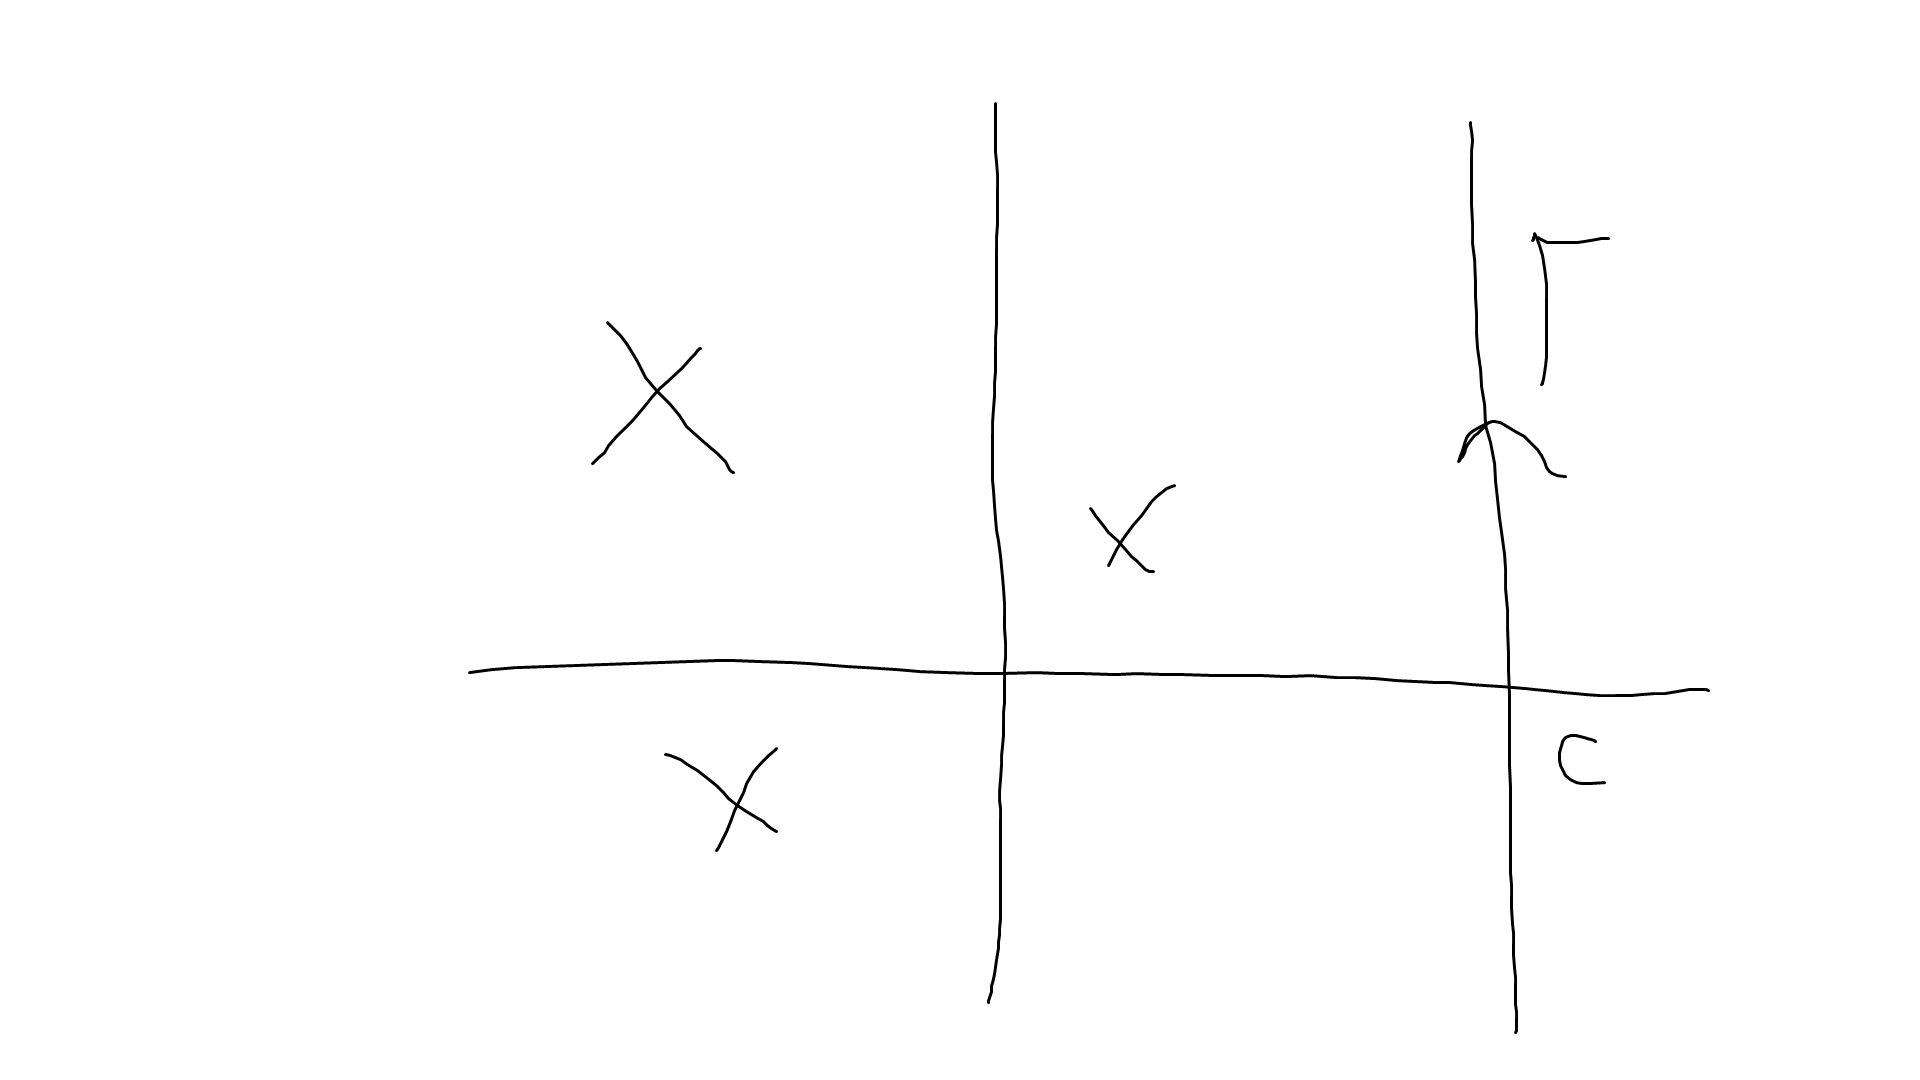
\includegraphics[scale=0.4]{CM_25}

In the case that $\hat{f}(p)$ has only a finite number of isolated singularities $p_k$, $k=1,...,n$, and $f(p) \to 0$ as $|p| \to \infty$,
\begin{equation*}
\begin{aligned}
f(t) = \sum_{k=1}^n res_{p=p_k} (\hat{f}(p) e^{pt})
\end{aligned}
\end{equation*}
for $t>0$, and vanishes for $t<0$.

Note that this result \emph{does not hold} if $\hat{f}(p) \not\to 0$ at $\infty$ (see example (iii) below).
\begin{proof}
When $t<0$, consider the contour $\gamma' = \gamma_0 + \gamma'_R$ shown, which encloses no singularities.

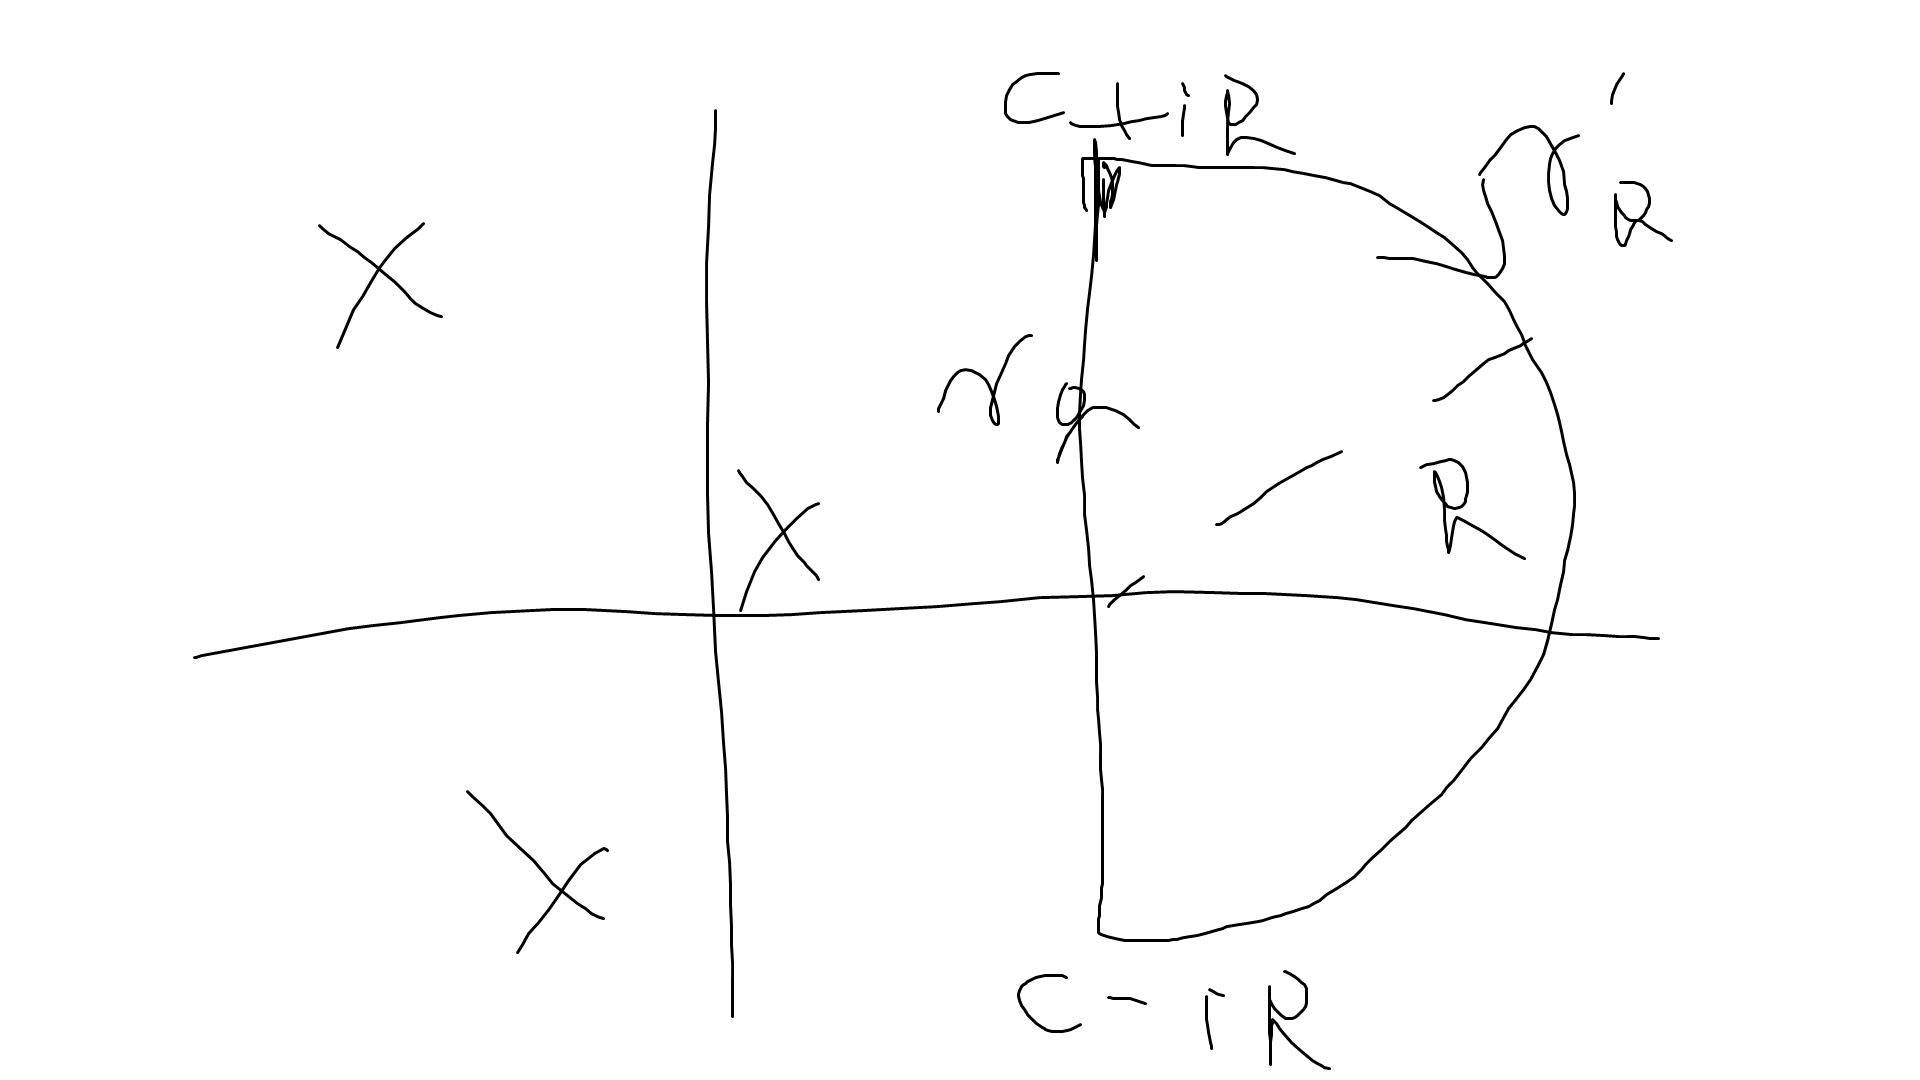
\includegraphics[scale=0.4]{CM_26}

If $\hat{f}(p) = o(|p|^{-1})$ as $|p|\to \infty$ then
\begin{equation*}
\begin{aligned}
\left|\int_{\gamma'_R} \hat{f}(p) e^{pt} dp\right| &\leq \pi R e^{ct} \sup_{p \in \gamma'_R} |\hat{f}(p)| \to 0
\end{aligned}
\end{equation*}
as $R \to \infty$ (here we have used $|e^{pt}| \leq e^ct$ which arises from the fact that $\Re(pt) \leq ct$, noting that $t<0$).

If $\hat{f}$ decays less rapidly at $\infty$, but still tends to zero there, the same result holds by a slight modification of Jordan's Lemma. So in either case, $\int_{\gamma'_R} \to 0$. Also, $\int_{\gamma_0} \to \int_\Gamma$; by Cauchy's theorem, therefore, $f(t) = 0$ for $t<0$ (As it must do for any function with a Laplace transform; this explains why $\Gamma$ must lie to the right of all the singularities).

When $t>0$, we close the contour to the left instead, and let $\gamma = \gamma_0+\gamma_R$ as shown. Once again we can show that $\int_{\gamma_R} \to 0$ as $R \to \infty$.

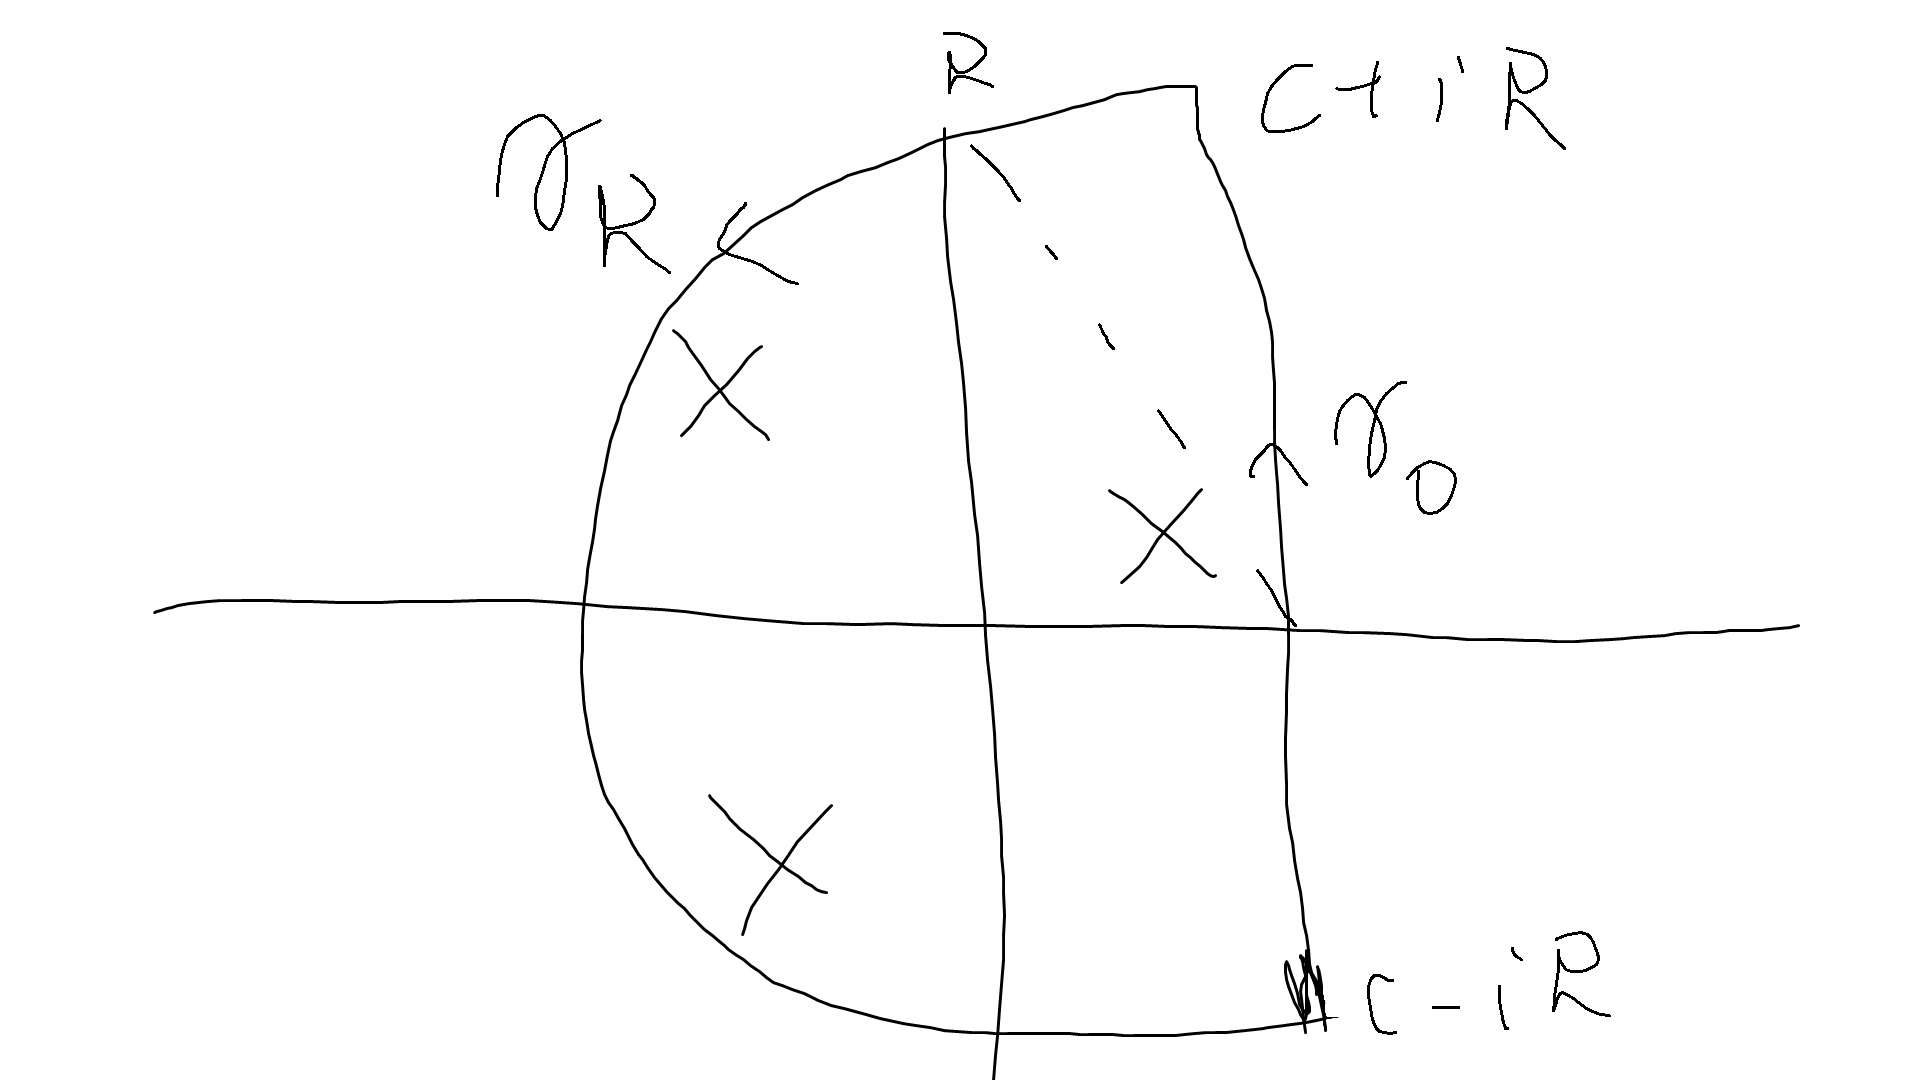
\includegraphics[scale=0.4]{CM_27}

Hence, by the residue theorem,
\begin{equation*}
\begin{aligned}
\int_\Gamma \hat{f}(p) e^pt dp &= \lim_{R \to \infty} \int_{\gamma_0}\hat{f}(p) e^pt dp\\
&= \lim_{R \to \infty} \int_{\gamma}\hat{f}(p) e^pt dp\\
&= 2\pi i \sum_{k=1}^n res_{p=p_k} (\hat{f}(p) e^{pt}).
\end{aligned}
\end{equation*}
The result follows (fiddly) from the Bromwich inversion formula.
\end{proof}

\begin{eg}
(i) $\hat{f}(p) = \frac{1}{p-1}$ has a pole at $p=1$, so we must use $c>1$. We have $\hat{f}(p) \to 0$ as $|p| \to \infty$, so Jordan's lemma applies as above. Hence $f(t) = 0$ for $t<0$, and for $t>0$, $$f(t) = res_{p=1} \left( \frac{e^{pt}}{p-1}\right) = e^t$$.

(ii) $\hat{f}(p) = p^{-n}$ has a pole of order $n$ at $p=0$, so $c>0$, and $\hat{f}(p) \to 0$ as $|p| \to \infty$. Hence for $t>0$, 
\begin{equation*}
\begin{aligned}
f(t) &= res_{p=0} \left(\frac{e^{pt}}{p^n}\right)\\
&= \lim_{p=0} \left\{ \frac{1}{(n-1)!} \frac{d^{n-1}}{dp^{n-1}} e^{pt} \right\}\\
&= \frac{t^{n-1}}{(n-1)!}.
\end{aligned}
\end{equation*}

(iii) In the case $\hat{f}(p) = \frac{e^{-p}}{p}$ we \emph{cannot} use the standard result above since $\hat{f}(p) \not\to 0$ as $|p| \to \infty$ in the left-hand half plane. But we can write
\begin{equation*}
\begin{aligned}
f(t) &= \frac{1}{2\pi i} \int_\Gamma \frac{e^{-p}}{p} e^{pt} dp\\
&= \frac{1}{2\pi i} \int_\Gamma \frac{1}{p} e^{pt'} dp
\end{aligned}
\end{equation*}
where $t' = t-1$. Now we can close to the right when $t'<0$ and to the left when $t'>0$, picking up the residue from the pole of $\frac{1}{p}$. Hence
\begin{equation*}
\begin{aligned}
f(t) &= \left\{ \begin{array}{ll}
0 & t'<0\\
1 & t'>0
\end{array}\right. \\&= \left\{ \begin{array}{ll}
0 & t<1\\
1 & t>1
\end{array}\right. \\&= H(t-1).
\end{aligned}
\end{equation*}

(iv) 

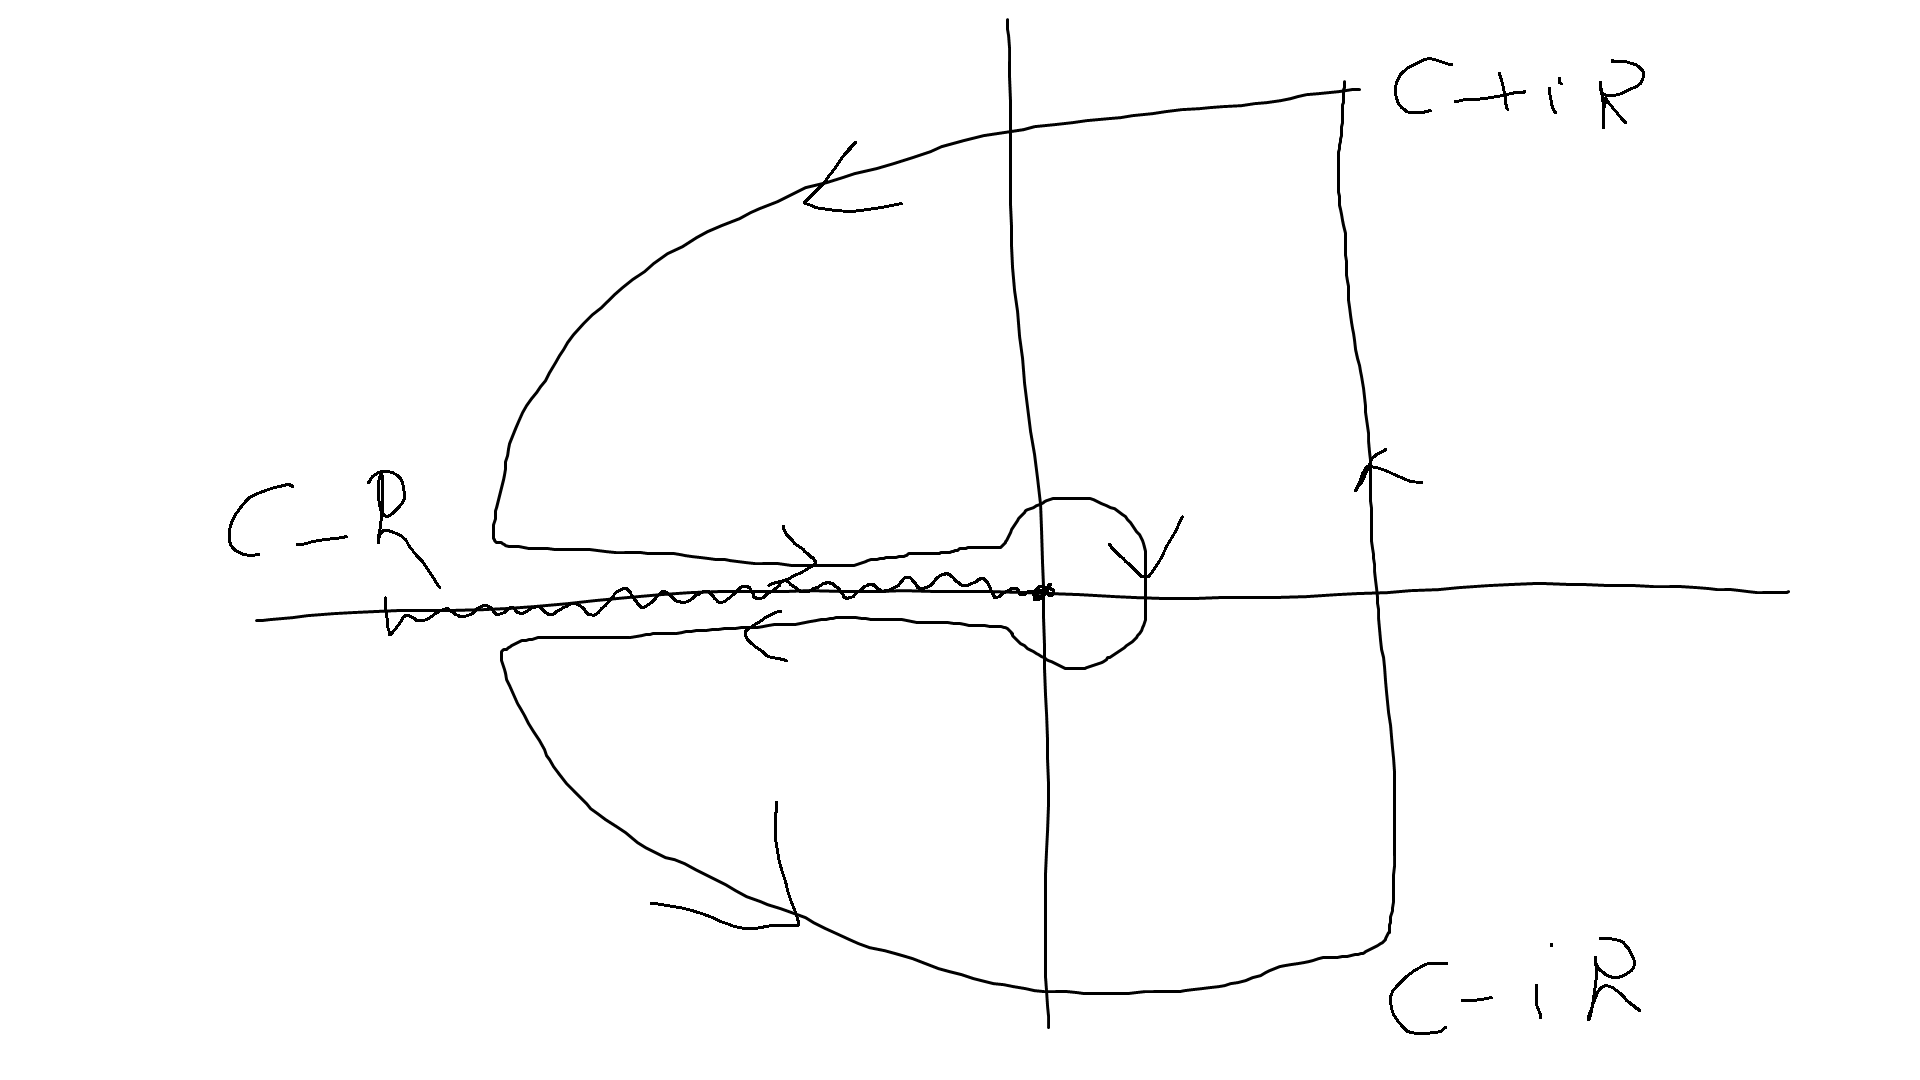
\includegraphics[scale=0.4]{CM_28}

If $\hat{f}(p)$ has a branch point (at $p=0$ say), then we must use a Bromwich keyhole contour as shown.
\end{eg}

\subsubsection{Derivation of the inverse Laplace transform (*)}

Since $f$ has a Laplace transform, it frows no more than exponentially fast; hence there exists $c \in \R$ s.t. 
\begin{equation*}
\begin{aligned}
g(t) = f(t) e^{-ct}
\end{aligned}
\end{equation*}
decays at $\infty$ (and is zero for $t<0$ of course). So $g$ has a Fourier transform and
\begin{equation*}
\begin{aligned}
\tilde{g}(w) = \int_{-\infty}^\infty f(t) e^{-ct} e^{-iwt} dt = \hat{f}(c+iw).
\end{aligned}
\end{equation*}
Then invert the Fourier transform, we get
\begin{equation*}
\begin{aligned}
g(t) &= \frac{1}{2\pi} \int_{-\infty}^\infty \hat{f}(c+iw) e^{iwt} dw
\\ \implies f(t) e^{-ct} &= \frac{1}{2\pi i} \int_{c-i\infty}^{c+i\infty} \hat{f}(p) e^{(p-c)t} dp 
\end{aligned}
\end{equation*}
by substituting $p=c+iw$. The result follows.

\subsection{The Convolution Theorem for Laplace Transforms}
The convolution of two functions $f$ and $g$
\begin{equation*}
\begin{aligned}
(f*g)(t) = \int_{-\infty}^\infty (t-t') g(t') dt'.
\end{aligned}
\end{equation*}
simplifies when $f$ and $g$ vanish for negative $t$ to
\begin{equation*}
\begin{aligned}
(f*g)(t) = \int_0^t f(t-t') g(t') dt'.
\end{aligned}
\end{equation*}
The convolution theorem states that $\mathcal{L}(f*g) (p) = \hat{f}(p) \hat{g}(p)$, just as for Fourier transforms.
\begin{proof}
\begin{equation*}
\begin{aligned}
\mathcal{L}(f*g) (p) &= \int_0^\infty \{\int_0^t f(t-t') g(t') dt' \} e^{-pt} dt\\
&= \int_0^\infty \{ \int_0^t f(t-t') g(t') e^{-pt} dt'\} dt\\
&= \int_0^\infty \{ \int_{t'}^\infty f(t-t') g(t') e^{-pt} dt\} dt'
\end{aligned}
\end{equation*}
by changing the order of integration in the $(t,t')$ plane, then equals
\begin{equation*}
\begin{aligned}
&\int_0^\infty \{ \int_0^\infty f(u) g(t') e^{-pu} e^{-pt'} du\} dt'\\
&= \int_0^\infty \{ \int_0^\infty f(u) e^{-pu} du\} g(t') e^{-pt'} dt'\\
&= \hat{f}(p) \hat{g}(p)
\end{aligned}
\end{equation*}
as required.
\end{proof}

\begin{eg}
If $f(t) = t$, then $\widehat{f*f} (p) = (\hat{f}(p))^2 = \frac{1}{p^4}$.

Now $\mathcal{L}(t^n) = \frac{n!}{p^{n+1}}$ (see section 5.2). So $(f*f) (t) = \frac{1}{6} t^3$. This is easily verified by direct calculation:
\begin{equation*}
\begin{aligned}
(f*f) (t) &= \int_0^t (t-t') t' dt'\\
&= \frac{1}{2} t^3 - \frac{1}{3}t^3 = \frac{1}{6}t^3.
\end{aligned}
\end{equation*}
\end{eg}

\subsection{Solution of Differential Equation using the Laplace Transform}
\begin{eg}
(i) The Laplace transform converts constant coefficient ODEs to algebraic equations (and PDEs to ODEs): see the worked example.

(ii) Consider
\begin{equation*}
\begin{aligned}
t\ddot{y} + (1-t)\dot{y} + 2y = 0, \ y(0) = 1.
\end{aligned}
\end{equation*}
Now
\begin{equation*}
\begin{aligned}
\mathcal{L}(t\dot{y}) &= -\frac{d}{dp}\mathcal{L}(\dot{y})\\
&= -\frac{d}{dp}(p\hat{y}-y(0))\\
&= -p\hat{y}'-y
\end{aligned}
\end{equation*}
using section 5.3 (vi) and (v). Similarly for $\mathcal{L}(t\ddot{y})$. hence we obtain (after simplification)
\begin{equation*}
\begin{aligned}
p(1-p)\hat{y}' = (p-3)\hat{y}
\end{aligned}
\end{equation*}
which is a first-order ODE for $\hat{y}(p)$. It is easily solved:
\begin{equation*}
\begin{aligned}
\hat{y} = A \left(\frac{1}{p} - \frac{2}{p^2} + \frac{1}{p^3}\right)
\end{aligned}
\end{equation*}
where $A$ is an arbitrary constant. Using section 5.3 (vii),
\begin{equation*}
\begin{aligned}
y(0) = \lim_{p \to \infty} p\hat{y}(p) = A
\end{aligned}
\end{equation*}
so $A=1$.

Inverting $\hat{y}$ using the 'library' in section 5.2 we get
\begin{equation*}
\begin{aligned}
y = 1 -2t + \frac{1}{2}t^2.
\end{aligned}
\end{equation*}
\end{eg}

\end{document}